\documentclass[12pt,a4paper,openany]{book}

% --- Encoding and fonts ---
\usepackage[utf8]{inputenc}
\usepackage[T1]{fontenc}
\usepackage{lmodern}

% --- Mathematics ---
\usepackage{amsmath}

% --- Page geometry ---
\usepackage[inner=2.5cm,outer=2.0cm,top=2.5cm,bottom=2.5cm]{geometry}

% --- Hyperlinks and automatic ToC ---
\usepackage[hidelinks]{hyperref}

% --- Index (via makeindex) ---
\usepackage{makeidx}
\makeindex

% --- Graphics (for future TikZ figures) ---
\usepackage{tikz}
\usetikzlibrary{positioning,arrows.meta,calc}

% --- Code listings ---
\usepackage{listings}
\lstdefinestyle{bookcode}{
    basicstyle=\ttfamily\footnotesize,
    frame=single,
    rulecolor=\color{black!40},
    breaklines=true,
    showstringspaces=false,
    aboveskip=8pt,
    belowskip=8pt,
    commentstyle=\itshape,
    columns=fullflexible,
}
\lstset{style=bookcode}

% --- Chapter headings style (optional; skipped if titlesec is missing) ---
\IfFileExists{titlesec.sty}{%
    \usepackage{titlesec}
    \titleformat{\chapter}[hang]{\Huge\bfseries}{\thechapter.\ }{0pt}{\Huge\bfseries}
}{}

% --- ToC depth ---
\setcounter{tocdepth}{2}   % show sections in ToC

\author{Daniel Castro}

\begin{document}

% ~~~~~~~~~~~~~~ Front matter ~~~~~~~~~~~~~~
\frontmatter
\title{\textbf{Transactional Memory\\[3mm]\Large From Principles to Practice}}
\author{A Comprehensive Guide}
\date{Version 0.1 -- \today}
\maketitle

\tableofcontents

\listoffigures
\listoftables
\lstlistoflistings

\chapter*{Preface}
\textbf{Assumed background.}
\begin{itemize}
    \item Computer architecture: caches, cache coherence, out-of-order execution (one semester).
    \item Operating systems / concurrency: threads, locks, semaphores, atomics.
    \item Compilers: a first course; the essential material is recapped in Part~V.
    \item Discrete mathematics and basic probability for the modeling parts (Part~III).
\end{itemize}
\textbf{How to read this book.}
\begin{itemize}
    \item Parts~I--II motivate TM and ground it in real hardware; readers with a strong OS/architecture background may skim them.
    \item Parts~III and IV (formal verification and runtime designs) are the conceptual core.
    \item Part~V (compilers) and Part~III (mathematics) are self-contained detours; their notation is reused later.
    \item A one-semester course could cover Parts~I, III, IV, and VI; a full course adds V and VII.
    \item A single running example --- a two-account \texttt{transfer()} --- threads through the book: it appears as locked code in Chapter~1, as an API call in Chapter~7, and as the test case for every runtime in Chapter~9.
\end{itemize}
\textbf{The companion codebase.}
\begin{itemize}
    \item This book is written against a working repository: 20+ STM backends, an LLVM instrumentation plugin, TLA+/PlusCal models, the STAMP benchmarks, and GPU backends.
    \item Exercises are tagged \emph{[implementation]} (write code), \emph{[verification]} (write a TLA+ model), or \emph{[theory]} (prove or derive) so instructors can mix them.
    \item Every runtime design in Part~IV exists as buildable code and as a model-checked TLA+ specification.
\end{itemize}
\textbf{Getting the code running.}
\begin{itemize}
    \item The full toolchain instructions live in the \emph{Development Environment Setup} chapter at the back; the minimum you need for most chapters is: \texttt{make} in the repository root (builds the backends and benchmarks), a recent \texttt{clang}/\texttt{g++} with C++17, and \texttt{java} plus the \texttt{tla2tools.jar} for the model-checking exercises.
    \item Exercise tracks: the tags let you follow one coherent path end-to-end. The \emph{implementer track} (all \emph{[implementation]}) builds a runtime of each family; the \emph{verifier track} (all \emph{[verification]}) builds a PlusCal/TLA+ model for each design; the \emph{theory track} (all \emph{[theory]}) carries the opacity and performance arguments across chapters. Each track's exercises are cumulative --- later ones reuse the artifacts of earlier ones.
\end{itemize}

\mainmatter

% -------------------------------------------------------------------
%  A MAP BEFORE PART I
% -------------------------------------------------------------------
\chapter*{A Map of Protocols and Acronyms}
\addcontentsline{toc}{chapter}{A Map of Protocols and Acronyms}
The same six-letter families recur throughout this book; pin them down once
here so later chapters can be read without re-decoding:

\begin{center}
\begin{tabular}{lp{4.2in}}
\textbf{Term} & \textbf{Meaning in this book} \\
\hline
TM & Transactional Memory (the concept, Ch.~1--2) \\
STM & Software TM: conflict detection in the runtime (Part~IV) \\
HTM & Hardware TM: conflict detection in the cache hierarchy (Ch.~16) \\
SGL & Single Global Lock --- the reference non-speculative design (Ch.~8) \\
TL2 & Global-clock, versioned-lock STM (Ch.~9) \\
NOrec & No Read-Lock, value-based validation (Ch.~9) \\
TinySTM & Lock-based STM with per-object locks (WBCTL/WT variants, Ch.~9) \\
JVSTM / MVLog & Multi-version STMs (Ch.~9) \\
PlusCal / TLA+ / TLC & Specification language, logic, and model checker (Ch.~6) \\
OCC / read-validate & Optimistic concurrency control; validate-then-write-back (Ch.~9) \\
RTM & Intel Restricted Transactional Memory (Ch.~16) \\
GUST & AtomicINC commit-log GPU TM (Ch.~17) \\
\end{tabular}
\end{center}

\section*{Why the book is ordered this way}
\begin{itemize}
    \item The order is deliberately \emph{not} ``hardware then software then
          formal then compilers.'' Mathematics and verification (Part~III)
          precede the runtimes (Part~IV) they specify, so that ``what a
          correct runtime must preserve'' is understood before ``what the
          runtime does with the calls.'' The runtimes in turn precede the
          compiler instrumentation (Part~V) that targets them, so the runtime
          ABI of Chapter~7 is fixed before ``what an instrumentation pass
          must preserve'' is read.
    \item Readers who prefer runtimes-first can start at Part~IV and consult
          Parts~III and V on demand; cross-references mark every such jump.
\end{itemize}

% -------------------------------------------------------------------
%  PART I: WHY TRANSACTIONAL MEMORY?
% -------------------------------------------------------------------
\part{Why Transactional Memory?}

\chapter{The Locking Crisis}
\section{The Cost of Mixing Synchronization with Logic}
\begin{itemize}
    \item Real-world examples: deadlocks, priority inversion, lost wake-ups.
    \item The tangling problem: concurrency control is scattered across the application.
    \item Readability, maintainability, and composability suffer.
    \item Three failure modes worth distinguishing: deadlock (no progress), livelock/starvation (no fairness), and data races (incorrectness).
    \item Locking contracts are \emph{invisible}: the compiler, the type system, and the reader cannot see which lock guards which variable.
    \item Error-prone patterns: check-then-act, test-and-set loops, nested locking, lock order inversion between modules.
    \item Heisenbugs: concurrency bugs reproduce only under specific interleavings, making them the costliest class of bugs in industry.
    \item Hidden costs beyond correctness: lock contention reduces parallelism, and coarse locking trades away scalability (Amdahl's law, revisited in Part~IV).
\end{itemize}

\section{Composability – The ``Innocent Change'' Problem}
\index{composability}
\begin{itemize}
    \item A small modification in one module breaks the locking protocol of another.
    \item Lock-based code is not composable; the whole call chain must obey the same locking order.
    \item The appeal of a declarative \texttt{atomic} block.
    \item Classic worked example: a thread-safe \texttt{List} and a thread-safe \texttt{Map}; transferring an element between them requires locking \emph{both} with a consistent global order.
    \item The ``innocent change'': adding one more field to a record silently inserts a second lock into a previously single-lock code path.
    \item Two independently correct modules can be combined into a deadlocking program --- no amount of local reasoning prevents it.
    \item Nesting should be \emph{free}: atomic blocks inside atomic blocks should compose by flattening rather than by a new locking protocol.
    \item TM removes the lock-order obligation: conflicts are detected at runtime on the accessed data, not by programmer-chosen lock order.
\end{itemize}

\section{Running Example: The Innocent Change in Code}

This book carries one small example through every chapter: a shared bank
account. It is small enough to fit in a listing and rich enough to exercise
every runtime in Part~IV. The first version is ``obviously correct'':

\begin{lstlisting}[language=C, caption={A locked transfer, ``obviously correct''.}]
void transfer(struct account *a, struct account *b, int n) {
    lock(&g_lock);
    a->balance -= n;
    b->balance += n;
    unlock(&g_lock);
}
\end{lstlisting}

Now the ``innocent change'': the business wants to reject a transfer that
would push either account below a floor, and the floor check acquires a
second lock:

\begin{lstlisting}[language=C, caption={The innocent change: two locks, an ordering obligation.}]
void transfer_safe(struct account *a, struct account *b, int n) {
    lock(&g_lock);
    lock(&g_floor_lock);               /* second lock, added later */
    int ok = (a->balance >= FLOOR) && (b->balance >= FLOOR);
    unlock(&g_floor_lock);
    if (!ok) { unlock(&g_lock); return; }
    a->balance -= n;
    b->balance += n;
    unlock(&g_lock);
}
\end{lstlisting}

Somewhere else, a ``check floor first'' path locks the two locks in the
opposite order --- and the program now deadlocks. The lesson of the previous
section, now in code the reader can compile. The transaction version needs no
ordering decision at all:

\begin{lstlisting}[language=C, caption={The same logic as a transaction.}]
__transaction_atomic {
    if (a->balance >= FLOOR && b->balance >= FLOOR) {
        a->balance -= n;
        b->balance += n;
    }
}
\end{lstlisting}

\begin{itemize}
    \item The transaction names the \emph{set of accesses}, not an order among them.
    \item The runtime detects conflicts on the data actually touched; the lock-order obligation is gone.
    \item The example returns in Chapters 7 and 9, where each runtime implements exactly these few lines.
\end{itemize}

\begin{figure}[htbp]
\centering
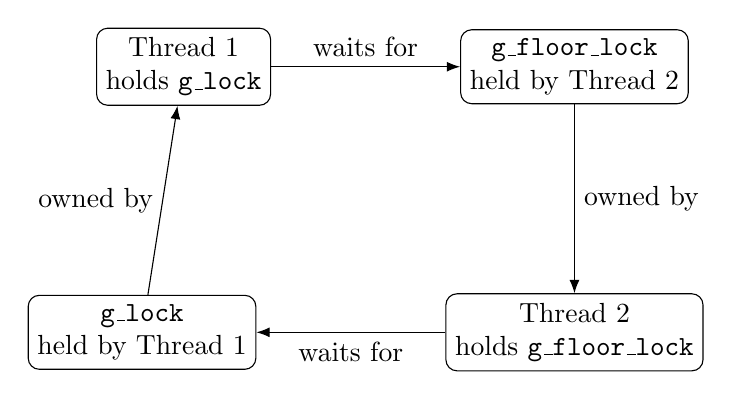
\begin{tikzpicture}[node distance=2.4cm, >=Latex]
    \node[draw, rounded corners, align=center] (t1) {Thread 1\\holds \texttt{g\_lock}};
    \node[draw, rounded corners, align=center, right=of t1] (floor) {\texttt{g\_floor\_lock}\\held by Thread 2};
    \node[draw, rounded corners, align=center, below=of floor] (t2) {Thread 2\\holds \texttt{g\_floor\_lock}};
    \node[draw, rounded corners, align=center, left=of t2] (g) {\texttt{g\_lock}\\held by Thread 1};

    \draw[->] (t1) -- node[above] {waits for} (floor);
    \draw[->] (floor) -- node[right] {owned by} (t2);
    \draw[->] (t2) -- node[below] {waits for} (g);
    \draw[->] (g) -- node[left] {owned by} (t1);
\end{tikzpicture}
\caption{A wait-for cycle created by opposite lock acquisition orders. Each edge is locally reasonable; the cycle is global.}
\label{fig:two-lock-deadlock}
\end{figure}

\begin{table}[htbp]
\centering
\begin{tabular}{p{0.23\linewidth} p{0.25\linewidth} p{0.25\linewidth} p{0.18\linewidth}}
\hline
Technique & Programmer obligation & Typical failure mode & Composability \\
\hline
Single global lock & Put every shared access under one lock. & Contention; accidental omissions. & Simple but not scalable. \\
Fine-grained locks & Maintain one global lock order across all modules. & Deadlock; lock-order inversion; priority inversion. & Brittle across module boundaries. \\
Try-lock and rollback & Write explicit failure and retry paths. & Livelock; starvation; duplicated recovery logic. & Better than blocking cycles, but non-local. \\
Transactional block & State the critical operation; let the runtime detect conflicts. & Abort and retry under contention. & Nested blocks can flatten. \\
\hline
\end{tabular}
\caption{Synchronization choices for the bank-transfer example. The table separates the correctness obligation from the mechanism used to enforce it.}
\label{tab:locking-crisis-taxonomy}
\end{table}

\section{Worked Example: Reproducing the Two-Lock Deadlock}

The following program is deliberately small. Both functions are locally
defensible: the transfer path protects balances first, then reads the floor;
the audit path reads the floor first, then checks balances. Together they
create the wait-for cycle in Figure~\ref{fig:two-lock-deadlock}.

\begin{lstlisting}[language=C, caption={A compilable two-lock deadlock. Build with: cc -std=c11 -pthread deadlock.c -o deadlock}]
#include <pthread.h>
#include <stdio.h>
#include <unistd.h>

struct account {
    int balance;
};

static pthread_mutex_t g_lock = PTHREAD_MUTEX_INITIALIZER;
static pthread_mutex_t g_floor_lock = PTHREAD_MUTEX_INITIALIZER;

static struct account alice = { .balance = 100 };
static struct account bob   = { .balance = 100 };
static int floor_value = 0;

static void transfer_safe(struct account *from,
                          struct account *to,
                          int amount) {
    pthread_mutex_lock(&g_lock);
    usleep(1000); /* widen the interleaving window */

    pthread_mutex_lock(&g_floor_lock);
    int ok = (from->balance - amount >= floor_value) &&
             (to->balance >= floor_value);
    pthread_mutex_unlock(&g_floor_lock);

    if (ok) {
        from->balance -= amount;
        to->balance += amount;
    }

    pthread_mutex_unlock(&g_lock);
}

static int audit_total_if_floors_hold(struct account *x,
                                      struct account *y) {
    int total = -1;

    pthread_mutex_lock(&g_floor_lock);
    usleep(1000); /* opposite order from transfer_safe */

    pthread_mutex_lock(&g_lock);
    if (x->balance >= floor_value && y->balance >= floor_value) {
        total = x->balance + y->balance;
    }
    pthread_mutex_unlock(&g_lock);

    pthread_mutex_unlock(&g_floor_lock);
    return total;
}

static void *transfer_thread(void *arg) {
    (void)arg;
    transfer_safe(&alice, &bob, 10);
    return NULL;
}

static void *audit_thread(void *arg) {
    (void)arg;
    int total = audit_total_if_floors_hold(&alice, &bob);
    printf("audit total = %d\n", total);
    return NULL;
}

int main(void) {
    pthread_t t1, t2;

    pthread_create(&t1, NULL, transfer_thread, NULL);
    pthread_create(&t2, NULL, audit_thread, NULL);

    pthread_join(t1, NULL);
    pthread_join(t2, NULL);

    printf("alice=%d bob=%d\n", alice.balance, bob.balance);
    return 0;
}
\end{lstlisting}

\begin{itemize}
    \item The bug is not in either critical section considered alone; it is in the composition.
    \item The sleep calls do not create the bug. They only make the bad interleaving easier to observe.
    \item Adding a second lock changed the public contract of \texttt{transfer\_safe}, even though the C type did not change.
    \item A global lock order can repair this program, but that order becomes an application-wide law.
\end{itemize}

\section{Worked Example: Model Checking the Bank Invariant}

The locking bug is an implementation artifact. The business rule is simpler:
an accepted transfer preserves total money and never leaves an account below
the floor. The following TLA+ module models that rule as one atomic step over
two accounts. TLC can check \texttt{MoneyInvariant} and
\texttt{FloorInvariant} by assigning, for example, \texttt{InitBal = 10},
\texttt{Floor = 0}, and \texttt{Amt = 1}.

\begin{lstlisting}[caption={A TLA+ model of atomic transfer and its invariants.}]
---- MODULE BankAtomic ----
EXTENDS Naturals

CONSTANTS InitBal, Floor, Amt
VARIABLES bal

Accounts == 1..2

Init ==
    /\ InitBal >= Floor
    /\ Amt > 0
    /\ bal = [i \in Accounts |-> InitBal]

CanTransfer(from, to) ==
    /\ from \in Accounts
    /\ to \in Accounts
    /\ from # to
    /\ bal[from] >= Floor + Amt
    /\ bal[to] >= Floor

DoTransfer(from, to) ==
    /\ CanTransfer(from, to)
    /\ bal' = [bal EXCEPT
        ![from] = @ - Amt,
        ![to]   = @ + Amt]

Next ==
    \E from, to \in Accounts:
        DoTransfer(from, to)

Spec == Init /\ [][Next]_bal

MoneyInvariant ==
    bal[1] + bal[2] = InitBal + InitBal

FloorInvariant ==
    \A i \in Accounts: bal[i] >= Floor

\* TLC invariants: MoneyInvariant, FloorInvariant
====
\end{lstlisting}

\begin{itemize}
    \item The model states the semantic invariant directly; it contains no mutexes and no lock order.
    \item The atomic step corresponds to the source-level transaction, not to a particular TM algorithm.
    \item Later chapters refine this step into concrete mechanisms: SGL, NOrec, TL2, TSC-TM, TinySTM, SwissTM, and the other backends all implement different conflict-detection and commit protocols.
    \item Verification should separate the application invariant from the synchronization mechanism whenever possible.
\end{itemize}

\section{Summary}
\begin{itemize}
    \item Locks are a powerful but dangerous tool.
    \item The software engineering argument for transactional memory is separation of concerns.
    \item Composability and locality of reasoning are the decisive advantages of transactions over locks.
\end{itemize}

\section{Exercises}
\begin{enumerate}
    \item Describe a scenario where two independently correct lock-based modules become deadlocked when combined. Propose a lock-free solution.
    \item Why does the priority inversion problem become worse in real-time systems? How could TM mitigate it?
    \item “Just use finer-grained locks” — discuss the limits of this advice.
    \item \emph{[implementation]} Compile the program in the first worked example. Replace the opposite-order audit path with a single global lock order, then with a \texttt{pthread\_mutex\_trylock} rollback path. Explain which version removes deadlock and which version can still starve.
    \item \emph{[verification]} Extend the TLA+ model with a rejected-transfer action that leaves \texttt{bal} unchanged when the floor check fails. Model check that \texttt{MoneyInvariant} and \texttt{FloorInvariant} are still inductive.
    \item \emph{[theory]} Give a precise argument for why nested locks do not compose automatically, while nested atomic blocks can be defined by flattening. State one assumption about the TM runtime that this argument requires.
\end{enumerate}

% -------------------------------------------------------------------
\index{composability}
\chapter{Transactions: From Databases to Shared Memory}
\index{transaction}\index{serializability}\index{ACID}
\section{ACID and Serializability}
\begin{itemize}
    \item Database transactions: Atomicity, Consistency, Isolation, Durability.
    \item Serializability as the gold standard for isolation.
    \item Why serializability is not directly transferable to in-memory concurrent programming.
    \item Database mechanisms we will reuse: version clocks, read/write sets, validation, write-ahead logging.
    \item The database-to-STM mapping: databases use disk-based logging and two-phase locking (2PL); STM replaces both with in-memory metadata and optimistic validation.
    \item Isolation levels (read committed, repeatable read, serializable) as a spectrum; TM typically targets the strongest end (opacity).
    \item In-memory difference: no durable media, no disk costs --- the cost centre shifts from I/O to coherence traffic and validation.
\end{itemize}

\section{Data Hazards and Memory Models}
\begin{itemize}
    \item Write-after-read, read-after-write, write-after-write hazards.
    \item Sequential consistency vs. relaxed memory models (TSO, RMO).
    \item How memory models affect the visibility of transactional writes.
    \item The three classical hazard classes (RAW, WAR, WAW) and how each maps to a transactional conflict.
    \item A transaction is really a sequence of hazards against other threads; concurrency control must resolve them consistently.
    \item Why relaxed models (TSO on x86, weak on ARM/GPUs) force TM implementations to insert fences; revisited from a compiler and runtime perspective in Parts~II, IV, and VII.
    \item The happens-before relation as the formal backbone for reasoning about visibility of committed writes.
\end{itemize}

\section{TM Semantics: Opacity, Sandboxing, Privatization}
\begin{itemize}
    \item Opacity: even aborted transactions must see a consistent view.
    \item The privatization anomaly: why serializability fails when transactions publish objects.
    \item Sandboxing: why speculative writes must not leak outside a transaction.
    \item Serializability vs.\ opacity: a history can be serializable while an aborted reader still observes an inconsistent partial state --- opacity closes that gap.
    \item Opacity also subsumes weak vs.\ strong atomicity debates via a single formal condition.
    \item Privatization: handing an object from a transactional context to a non-transactional one must publish a consistent version; naive STMs corrupt it.
    \item Sandboxing: instrumentation, not hardware, must guarantee that accesses outside a transaction are never redirected to speculative state.
    \item The three conditions are the yardstick used to model-check every backend in Part~III (see, e.g., the \texttt{InvNoMissedConflict} invariant of Part~VII).
\end{itemize}

\begin{figure}[htbp]
\centering
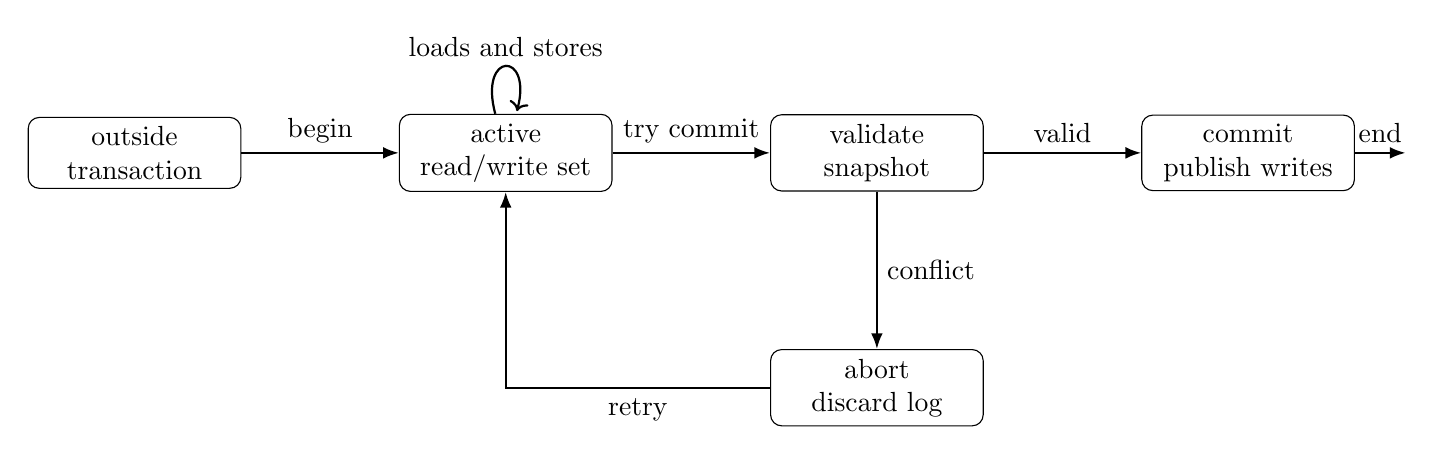
\begin{tikzpicture}[
    node distance=2.0cm,
    state/.style={draw, rounded corners, minimum width=2.7cm, minimum height=0.9cm, align=center},
    edge/.style={-{Latex[length=2mm]}, thick}
]
\node[state] (idle) {outside\\transaction};
\node[state, right=of idle] (active) {active\\read/write set};
\node[state, right=of active] (validate) {validate\\snapshot};
\node[state, right=of validate] (commit) {commit\\publish writes};
\node[state, below=of validate] (abort) {abort\\discard log};

\draw[edge] (idle) -- node[above]{begin} (active);
\draw[edge] (active) -- node[above]{try commit} (validate);
\draw[edge] (validate) -- node[above]{valid} (commit);
\draw[edge] (commit) -- node[above]{end} ($(commit)+(2.0,0)$);
\draw[edge] (validate) -- node[right]{conflict} (abort);
\draw[edge] (abort) -| node[pos=0.25, below]{retry} (active);
\draw[edge] (active) edge[loop above] node{loads and stores} (active);
\end{tikzpicture}
\caption{A minimal transactional state machine for the bank example. The programmer marks the operation boundary; the runtime records accesses, validates the observed snapshot, and either publishes all writes or discards them.}
\label{fig:transactional-state-machine}
\end{figure}

\begin{table}[htbp]
\centering
\begin{tabular}{p{0.18\linewidth} p{0.22\linewidth} p{0.27\linewidth} p{0.23\linewidth}}
\hline
Family & Examples in the codebase & Serialization point & Bank-transfer consequence \\
\hline
Coarse lock & SGL, PersistentSGL, DistributedSGL & Lock acquisition or durable lock protocol & Simple proof; poor scalability under independent transfers. \\
Hardware fast path & TSX-SGL & Hardware transaction commit, with SGL fallback & Fast when transactions fit hardware limits; fallback preserves correctness. \\
Versioned STM & NOrec, NOrec-BF, TL2, TSC-TM & Global clock or per-object version validation & Detects stale reads of balances or floors before publishing writes. \\
Multi-version STM & JVSTM, MVLog & Version selection plus commit validation & Readers can observe older committed versions while writers proceed. \\
Persistent or distributed TM & NV-HTM, Romulus, XTM, TiKV & Durable commit record or distributed commit decision & Atomicity must include recovery or participant agreement. \\
GPU TM & PR-STM, CSMV, GPUTX, GAccO, GPU-JVSTM, GUST & Kernel-level commit protocol or commit log & Conflicts are batched across many lightweight threads. \\
\hline
\end{tabular}
\caption{Transactional implementations differ mainly in where they serialize a transaction and how they validate the read set. The companion implementations all pass the same bank-style correctness tests, but expose different performance envelopes.}
\label{tab:tm-family-taxonomy}
\end{table}

\section{Worked Example: A History That Is Serializable but Not Opaque}
\index{opacity}\index{serializable but not opaque}\index{serializability}\index{linearizability}\index{strict serializability}\index{weak atomicity}\index{strong atomicity}\index{commit order}\index{read-set}\index{write-set}\index{validation}\index{conflict detection}\index{version management}\index{write-back}\index{undo log}\index{commit lock}\index{OCC}\index{eager version management}\index{lazy version management}

Consider two transactions $T_1$ and $T_2$ operating on locations $x$ and
$y$, both initially 0. The following interleaving is \emph{serializable}
yet \emph{not opaque}:

\begin{lstlisting}[caption={A serializable-but-not-opaque history.}]
T1: read x = 0            // 1. T1 reads x = 0 (old value)
T2: write x = 1           // 2. T2 writes x = 1
T2: write y = 1           // 3. T2 writes y = 1
T2: commit                // 4. T2 commits: state is now (x,y) = (1,1)
T1: read y = 1            // 5. T1 reads the *fresh* y = 1
T1: abort                 // 6. T1 aborts
\end{lstlisting}

\begin{itemize}
    \item Only $T_2$ commits, so the committed history is trivially serializable --- an aborted $T_1$ is simply dropped from the serial order.
    \item But $T_1$ read $x = 0$ \emph{and then} $y = 1$: the combination $(x,y) = (0,1)$ never existed at any single moment. A state that never existed was observed.
    \item Opacity forbids this: even an aborted transaction must read a state that lies on some valid serialization. Serializability alone says nothing about aborted transactions.
    \item This is the precise gap the invariants of Part~III encode, e.g.\ \texttt{InvNoMissedConflict} in the GPU chapter.
    \item We will re-run this exact history on NOrec and TL2 in Chapter~9 to see where opacity is enforced --- and, in the exercises, against a deliberately broken runtime to see where it leaks.
\end{itemize}

\section{Worked Example: A Minimal Litmus-Test Harness}
\index{litmus test}\index{invariant test}
The history above is one instance of a general technique the book reuses
from here to the GPU chapter: a \emph{litmus test}.  A litmus test is a
tiny, fixed schedule that either must commit or must abort for the
implementation to be correct.  The harness is a few lines that run the
schedule, run a reference serialization, and compare:

\begin{lstlisting}[language=C, caption={A litmus-test harness reused by every protocol chapter.}]
struct result run_litmus(schedule_fn f, serialize_fn ref) {
    struct result r = f();          /* execute the schedule on the TM */
    return (r.serializable == ref(r)) ? r : (struct result){ .abort = 1 };
}
\end{lstlisting}

\begin{itemize}
    \item Each chapter that introduces a runtime (11, 12, 16, 17) ships the \emph{same} litmus tests, so a regression in any backend is a one-line change to spot.
    \item A litmus test has three parts: a fixed thread schedule, an assertion about the committed result, and the corresponding serial-order check.
    \item The invariant tests of Chapter~12 (e.g.\ the money-conservation test) are litmus tests made stochastic: the schedule is randomized, the assertion is the invariant.
\end{itemize}

\section{Worked Example: Flattening Nested Bank Transactions}

A single global lock is not a scalable STM, but it is a precise executable
model of the transactional interface. The important property in this example
is \emph{flattening}\index{nested transaction!flattening}: a nested transaction
does not acquire the lock again and does not commit independently.

\begin{lstlisting}[language=C, caption={A compilable flattened transaction wrapper. Build with: cc -std=c11 -pthread tx\_flatten.c -o tx\_flatten}]
#include <assert.h>
#include <pthread.h>
#include <stdio.h>

struct account {
    int balance;
};

static pthread_mutex_t tx_lock = PTHREAD_MUTEX_INITIALIZER;
static _Thread_local int tx_depth = 0;

static struct account alice = { .balance = 100 };
static struct account bob   = { .balance = 100 };
static int floor_value = 0;
static const int initial_total = 200;

static void tx_begin(void) {
    if (tx_depth == 0) {
        pthread_mutex_lock(&tx_lock);
    }
    tx_depth++;
}

static void tx_end(void) {
    assert(tx_depth > 0);
    tx_depth--;
    if (tx_depth == 0) {
        pthread_mutex_unlock(&tx_lock);
    }
}

static int total_unlocked(void) {
    return alice.balance + bob.balance;
}

static int transfer_tx(struct account *from,
                       struct account *to,
                       int amount) {
    int committed = 0;

    tx_begin();

    if (from->balance - amount >= floor_value &&
        to->balance >= floor_value) {
        from->balance -= amount;
        to->balance += amount;
        committed = 1;
    }

    assert(total_unlocked() == initial_total);

    tx_end();
    return committed;
}

static int audit_total_tx(void) {
    int total;

    tx_begin();

    if (alice.balance >= floor_value && bob.balance >= floor_value) {
        total = total_unlocked();
    } else {
        total = -1;
    }

    tx_end();
    return total;
}

static void payroll_tx(void) {
    tx_begin();

    (void)transfer_tx(&alice, &bob, 10);
    (void)transfer_tx(&bob, &alice, 5);

    int total = audit_total_tx();
    assert(total == -1 || total == initial_total);

    tx_end();
}

int main(void) {
    payroll_tx();

    printf("alice=%d bob=%d total=%d\n",
           alice.balance, bob.balance, audit_total_tx());

    return 0;
}
\end{lstlisting}

Lessons:

\begin{itemize}
    \item The outer transaction is the only real synchronization boundary.
    \item Inner transactions are ordinary function calls with atomicity inherited from the enclosing transaction.
    \item The money-conservation assertion is checked while the lock is held, so it observes a stable state.
    \item This SGL implementation is useful as a reference backend and oracle, not as the performance target.
\end{itemize}

\section{Worked Example: Model Checking Money Conservation}

The locking example shows an execution bug. The corresponding specification
states the intended atomic step directly: a transfer changes both balances in
one transition. TLC can check the money-conservation and floor invariants for
all reachable states under a fixed floor.

\begin{lstlisting}[language={}, caption={A TLA+ model of atomic bank transfers. Save as BankTransferInvariant.tla and run TLC with Floor set to 0.}]
---- MODULE BankTransferInvariant ----
EXTENDS Naturals, TLC

CONSTANT Floor

VARIABLES alice, bob

vars == << alice, bob >>

Init ==
    /\ alice = 100
    /\ bob = 100
    /\ alice >= Floor
    /\ bob >= Floor

CanDebit(x) ==
    x >= 10 + Floor

TransferAB ==
    /\ CanDebit(alice)
    /\ alice' = alice - 10
    /\ bob' = bob + 10

TransferBA ==
    /\ CanDebit(bob)
    /\ bob' = bob - 10
    /\ alice' = alice + 10

Next ==
    \/ TransferAB
    \/ TransferBA
    \/ UNCHANGED vars

Spec ==
    Init /\ [][Next]_vars

TypeOK ==
    /\ alice \in Nat
    /\ bob \in Nat

MoneyConserved ==
    alice + bob = 200

FloorsHold ==
    /\ alice >= Floor
    /\ bob >= Floor

=============================================================================
\end{lstlisting}

A minimal TLC configuration is:

\begin{lstlisting}[language={}, caption={TLC configuration for the bank-transfer invariant. Save as BankTransferInvariant.cfg.}]
CONSTANT
    Floor = 0

SPECIFICATION
    Spec

INVARIANTS
    TypeOK
    MoneyConserved
    FloorsHold
\end{lstlisting}

Lessons:

\begin{itemize}
    \item The specification has no locks. It describes the atomic state transition.
    \item Splitting debit and credit into separate actions makes \texttt{MoneyConserved} fail immediately.
    \item The floor invariant is a precondition on debit, not a post-hoc repair.
    \item The implementation may use locks, versions, hardware transactions, or a commit log, but it must refine this atomic behavior.
\end{itemize}

\section{Summary}
\begin{itemize}
    \item Database isolation does not directly solve shared-memory concurrency problems.
    \item TM correctness requires stronger conditions like opacity.
\end{itemize}

\section{Exercises}
\begin{enumerate}
    \item Construct a history of three transactions that is serializable but not opaque.
    \item Explain why a TM that uses simple timestamp ordering without validation can produce a non-serializable outcome.
    \item Discuss the performance implications of enforcing opacity in hardware vs. software.
    \item \emph{[implementation]} Replace the single global lock in the flattened wrapper's execution model with a small redo-log STM for two accounts. Reads should return speculative writes from the log before consulting memory. Commit should validate that both logged source balances still equal the values read at transaction start, then publish both writes while holding one commit mutex.
    \item \emph{[verification]} Extend \texttt{BankTransferInvariant.tla} with a deliberately broken two-step transfer: one action debits Alice and a later action credits Bob. Check that the invariant $\sum_{\text{account}} \text{balance} = 200$ fails. Then repair the model by adding an explicit pending-transfer record and write the corrected conservation invariant over both balances and the pending amount.
    \item \emph{[theory]} The table in \S\ref{tab:tm-family-taxonomy} separates serialization points from validation mechanisms. For each of SGL, TL2, NOrec, and a multi-version STM, state where the transaction linearizes in a successful bank transfer. Then explain whether a read-only audit can linearize without blocking a concurrent writer.
\end{enumerate}

% -------------------------------------------------------------------
%  PART II: THE MACHINE BENEATH
% -------------------------------------------------------------------
\part{The Machine Beneath}
\index{opacity}\index{serializable but not opaque}\index{serializability}\index{linearizability}\index{strict serializability}\index{weak atomicity}\index{strong atomicity}\index{commit order}\index{read-set}\index{write-set}\index{validation}\index{conflict detection}\index{version management}\index{write-back}\index{undo log}\index{commit lock}\index{OCC}\index{eager version management}\index{lazy version management}

\chapter{Hardware Concepts for Transactional Memory}
\section{Multicore Architectures and Memory Hierarchies}
\begin{itemize}
    \item Shared memory, caches (L1/L2/L3), cache coherence (MESI).
    \item The coherence protocol as a natural conflict‑detection substrate.
    \item MESI states and transitions: a cache line invalidated by another core is, from a TM viewpoint, a conflict signal.
    \item Snooping vs.\ directory‑based coherence, and a first look at why coherence does not exist across GPU SMs (Part~VII).
    \item Word vs.\ cache‑line granularity of conflict detection: where false conflicts come from (Part~VII).
\end{itemize}

\section{Out-of-Order Execution and Speculation}
\begin{itemize}
    \item Instruction pipelines, reorder buffers, branch prediction.
    \item Speculative stores and why they can be squashed.
    \item The reorder buffer holds register state, not data; hardware TM must own speculative data in the cache.
    \item Capacity limits: the transaction working set is bounded by L1; larger transactions need software transactions or fallback.
    \item The parallel between branch misprediction recovery and transactional abort.
\end{itemize}

\section{Store Buffers and Memory Ordering}
\begin{itemize}
    \item How store buffers relax write-to-read ordering (TSO).
    \item Memory fences and their cost.
    \item Why a purely software TM must insert fences on some architectures.
    \item The commit-publish fence: a transaction's write‑back must become visible in one atomic step to other cores.
    \item Compiler fences (\texttt{atomic\_signal\_fence}) vs.\ hardware fences (\texttt{mfence}, \texttt{dmb}): eliminating the CPU barrier on the read path (Part~IV).
    \item Fence placement as a correctness issue, not a tweak: wrong placement reopens the commit-visibility window.
\end{itemize}

\section{Worked Example: The TSO Store-Buffer Surprise}
\index{TSO}\index{store buffer}\index{memory model}\index{data race}\index{happens-before}\index{fence}\index{compiler barrier}\index{acquire/release}\index{seq\_cst}
\label{sec:tso-example}

The running bank example can expose a memory-ordering subtlety. Consider a
transfer that writes to account~$A$ and then reads account~$B$:

\begin{lstlisting}[language=C, caption={A transfer that writes then reads.}]
void transfer_and_check(account_t *a, account_t *b, int n) {
    a->balance -= n;        /* 1. speculative write to A  */
    if (b->balance < n)     /* 2. read from B             */
        rollback(a, n);     /* 3. undo the write          */
}
\end{lstlisting}

\begin{itemize}
    \item On TSO (x86), the store to \texttt{A} sits in the store buffer; the subsequent load of \texttt{B} can be satisfied before \texttt{A} is visible to other cores.
    \item A concurrent thread can observe $A$ updated while $B$ is still the old value --- a torn view of the transaction.
    \item The fix is a release fence on commit: the write-back of the whole write-set must become visible at once.
    \item This is the store-buffer echo of the \emph{snapshot consistency} problem, revisited in Part~IV for software TM and Part~VII for GPUs.
    \item Exercise~2 of this chapter asks you to draw the precise interleaving.
\end{itemize}

\begin{figure}[ht]
\centering
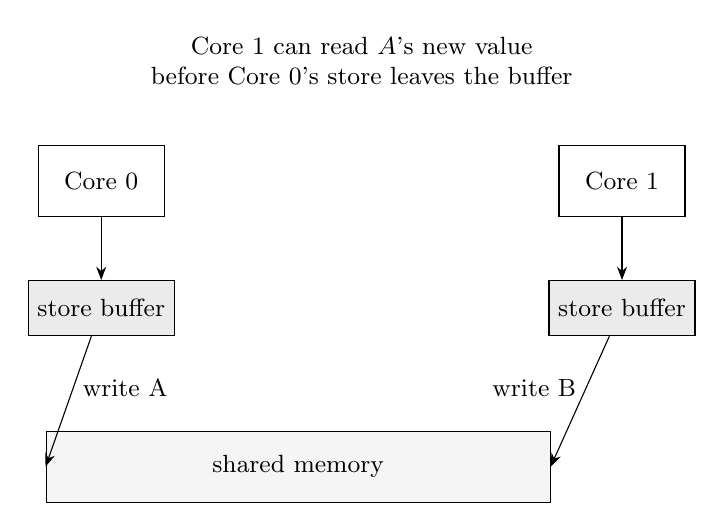
\begin{tikzpicture}[font=\small]
  % two cores with a store buffer between them
  \node[draw,rectangle,minimum width=1.6cm,minimum height=0.9cm] (coreA) {Core 0};
  \node[draw,rectangle,minimum width=1.6cm,minimum height=0.9cm] (coreB) [right=5cm of coreA] {Core 1};
  \node[draw,rectangle,minimum width=1.4cm,minimum height=0.7cm,fill=black!8] (sbA) [below=0.8cm of coreA] {store buffer};
  \node[draw,rectangle,minimum width=1.4cm,minimum height=0.7cm,fill=black!8] (sbB) [below=0.8cm of coreB] {store buffer};
  \draw[-{Stealth}] (coreA) -- (sbA);
  \draw[-{Stealth}] (coreB) -- (sbB);
  \node[draw,rectangle,minimum width=6.4cm,minimum height=0.9cm,fill=black!4] (mem) [below=1.2cm of sbA,xshift=2.5cm] {shared memory};
  \draw[-{Stealth}] (sbA) -- node[right,pos=0.4] {write A} (mem.west);
  \draw[-{Stealth}] (sbB) -- node[left,pos=0.4] {write B} (mem.east);
  % the torn view
  \node[align=center,text width=6cm] at ($(coreA)!0.5!(coreB)$) [above=0.5cm,yshift=0.6cm]
        {Core 1 can read $A$'s new value\\before Core 0's store leaves the buffer};
\end{tikzpicture}
\caption{The TSO store-buffer reordering hazard: the write to $A$ (Core~0) and the write to $B$ (Core~1) can become visible in the opposite order, so an observer can see $A$ updated while $B$ is stale.}
\label{fig:tso-store-buffer}
\end{figure}

\section{Worked Example: Cache-Line False Conflicts}
\index{false conflict}\index{cache line}\index{conflict detection}\index{HTM}

Hardware transactional memory normally detects conflicts at cache-line
granularity. Two independent accounts can conflict if they share a line, even
when no transaction touches the same word. The following program is not a TM
implementation; it is a layout check for the data structure that a TM backend
will execute on top of.

\begin{lstlisting}[language=C++, caption={Separating bank accounts onto cache lines.}]
#include <atomic>
#include <cassert>
#include <cstdint>
#include <iostream>
#include <mutex>

static constexpr std::size_t CACHE_LINE = 64;

struct Account {
    std::atomic<int> balance;
};

/* One logical account per coherence block. */
struct alignas(CACHE_LINE) PaddedAccount {
    std::atomic<int> balance;
    char padding[CACHE_LINE - sizeof(std::atomic<int>)];
};

static_assert(sizeof(PaddedAccount) % CACHE_LINE == 0,
              "padded accounts must not straddle cache-line slots");

template <typename A>
bool transfer_sgl(A& from, A& to, int amount) {
    static std::mutex global_lock;
    std::lock_guard<std::mutex> guard(global_lock);

    int old_from = from.balance.load(std::memory_order_relaxed);
    if (old_from < amount) return false;

    from.balance.store(old_from - amount, std::memory_order_relaxed);
    to.balance.fetch_add(amount, std::memory_order_relaxed);
    return true;
}

static std::uintptr_t line_of(const void* p) {
    return reinterpret_cast<std::uintptr_t>(p) / CACHE_LINE;
}

int main() {
    Account compact[2] = {{100}, {100}};
    PaddedAccount padded[2] = {{100}, {100}};

    std::cout << "compact lines: "
              << line_of(&compact[0]) << " "
              << line_of(&compact[1]) << "\n";

    std::cout << "padded lines:  "
              << line_of(&padded[0]) << " "
              << line_of(&padded[1]) << "\n";

    assert(line_of(&padded[0]) != line_of(&padded[1]));

    bool ok = transfer_sgl(padded[0], padded[1], 30);
    assert(ok);
    assert(padded[0].balance.load() + padded[1].balance.load() == 200);
}
\end{lstlisting}

\begin{itemize}
    \item Coherence works on blocks, not abstract objects. HTM conflict detection inherits that granularity.
    \item Padding can reduce false conflicts, but it increases footprint and can increase capacity aborts.
    \item SGL-style execution is insensitive to false conflicts, but it also removes concurrent execution.
    \item TSX-SGL uses HTM when the hardware accepts the transaction and falls back to a single global lock when it does not.
\end{itemize}

\section{HTM Execution States}
\index{TSX}\index{capacity abort}\index{fallback path}\index{single global lock}

\begin{figure}[htbp]
\centering
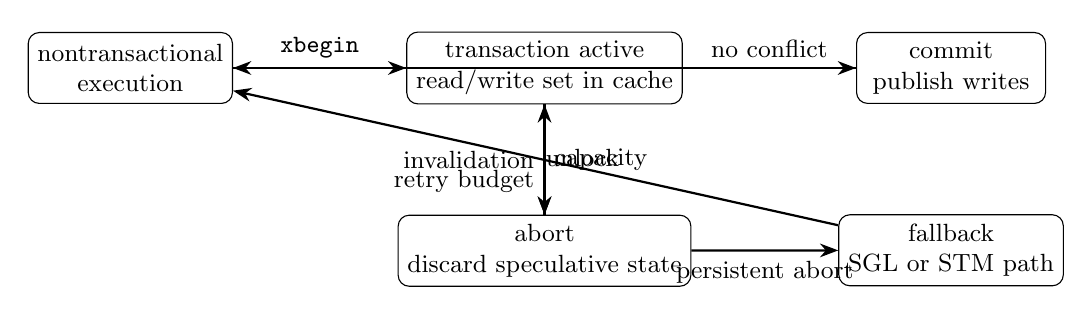
\begin{tikzpicture}[
    font=\small,
    state/.style={draw,rectangle,rounded corners,align=center,
                  minimum width=2.4cm,minimum height=0.9cm},
    edge/.style={-{Stealth},thick}
]
  \node[state] (idle) {nontransactional\\execution};
  \node[state,right=2.2cm of idle] (active) {transaction active\\read/write set in cache};
  \node[state,right=2.2cm of active] (commit) {commit\\publish writes};
  \node[state,below=1.4cm of active] (abort) {abort\\discard speculative state};
  \node[state,below=1.4cm of commit] (fallback) {fallback\\SGL or STM path};

  \draw[edge] (idle) -- node[above] {\texttt{xbegin}} (active);
  \draw[edge] (active) -- node[above] {no conflict} (commit);
  \draw[edge] (commit) -- node[above,bend left=10] {} (idle);
  \draw[edge] (active) -- node[left] {invalidation} (abort);
  \draw[edge] (active) -- node[right] {capacity} (abort);
  \draw[edge] (abort) -- node[below left] {retry budget} (active);
  \draw[edge] (abort) -- node[below] {persistent abort} (fallback);
  \draw[edge] (fallback) -- node[right] {unlock} (idle);
\end{tikzpicture}
\caption{A minimal HTM state machine. Speculative data live in the cache while the transaction is active. Coherence invalidations and capacity overflow abort the transaction; robust implementations include a fallback path.}
\label{fig:htm-state-machine}
\end{figure}

\section{Worked Example: Atomic Commit-Publish in TLA+}
\index{TLA+}\index{commit-publish}\index{invariant}\index{money conservation}

The hardware rule ``publish all writes at commit'' has a direct specification
counterpart: the transfer is one next-state action. The debit and the credit
are not separate visible steps.

\begin{lstlisting}[caption={A finite TLA+ model of atomic bank transfers.}]
-------------------------- MODULE BankAtomicCommit --------------------------
EXTENDS Naturals

VARIABLE balance

Accounts == {"A", "B"}

Init ==
    balance = ["A" |-> 100, "B" |-> 100]

Transfer(a, b, n) ==
    /\ a \in Accounts
    /\ b \in Accounts
    /\ a # b
    /\ n \in 1..10
    /\ balance[a] >= n
    /\ balance' =
        [balance EXCEPT
            ![a] = @ - n,
            ![b] = @ + n]

Next ==
    \E a \in Accounts:
    \E b \in Accounts:
    \E n \in 1..10:
        Transfer(a, b, n)

Total == balance["A"] + balance["B"]

FloorOK ==
    \A a \in Accounts: balance[a] >= 0

Invariant ==
    /\ Total = 200
    /\ FloorOK

Spec ==
    Init /\ [][Next]_balance
=============================================================================
\end{lstlisting}

\begin{itemize}
    \item The write-set is modeled by the function update in \texttt{balance'}.
    \item The invariant combines money conservation and the account floor property.
    \item If the transfer is split into a visible debit action followed by a visible credit action, TLC can reach an intermediate state that violates money conservation.
    \item The same atomicity obligation appears in software TM write-back, HTM commit, persistent TM log replay, and distributed two-phase commit.
\end{itemize}

\section{Hardware Mechanisms and TM Consequences}

\begin{table}[htbp]
\centering
\begin{tabular}{p{0.24\linewidth}p{0.31\linewidth}p{0.34\linewidth}}
\hline
Mechanism & TM consequence & Representative backends in the codebase \\
\hline
Cache coherence & Natural conflict signal for HTM; invalidation of a read or write line aborts the transaction. False conflicts arise at cache-line granularity. & TSX-SGL; also relevant to TL2, NOrec, and TSC-TM because their metadata and payload placement affect cache traffic. \\
\hline
Private L1 cache & Bounds the speculative footprint of HTM transactions. Large read/write sets may abort even without a logical conflict. & TSX-SGL falls back to SGL; larger software paths include TL2, NOrec, NOrec-BF, TinySTM variants, and SwissTM. \\
\hline
Store buffer & Delays visibility of stores; software write-back needs correct publish ordering and fences. & NOrec, TL2, TSC-TM, TinySTM WBCTL/WT/WBETL, SwissTM. \\
\hline
Timestamp counter or logical clock & Enables version validation and fast read paths, but clock reads and ordering must match the memory model. & TL2, TSC-TM, NOrec, JVSTM, MVLog. \\
\hline
No coherent cache across GPU SMs & Conflict detection cannot be borrowed directly from MESI; validation and commit protocols must be explicit. & PR-STM, CSMV, GPUTX, GAccO, GPU-JVSTM, GUST. \\
\hline
Persistent memory ordering & Commit must survive crashes as an all-or-nothing durable transition. Flushes and persist barriers become part of correctness. & NV-HTM, Romulus, PersistentSGL. \\
\hline
Distributed memory & Coherence is replaced by messages, locks, leases, timestamps, or consensus-adjacent protocols. & DistributedSGL and TiKV-style Percolator two-phase commit. \\
\hline
\end{tabular}
\caption{Hardware and platform mechanisms as they appear in TM design. The same bank invariant is simple; the publication substrate changes.}
\label{tab:hardware-tm-taxonomy}
\end{table}

\section{Summary}
\begin{itemize}
    \item Modern CPUs already implement a form of speculative rollback.
    \item Cache coherence can detect conflicts, but store buffers hide visibility.
\end{itemize}

\section{Exercises}
\begin{enumerate}
    \item Draw a pipeline diagram showing a speculatively executed store that must be squashed on an abort.
    \item In a system with TSO, a transaction writes to location A and then reads B. Show a scenario where another thread sees the write to A before the transaction commits, violating opacity. Propose a fence placement.
    \item Explain why a TM that uses only cache coherence for conflict detection might still suffer from store-buffer effects.
    \item \emph{[implementation]} Modify the cache-line example so that four worker threads repeatedly transfer between adjacent accounts. Provide two layouts: compact and padded. Count committed transfers only under the SGL wrapper, and check after every run that the total balance is unchanged. Do not report timing as a research result; use the experiment only to inspect layout and contention.
    \item \emph{[verification]} Extend the TLA+ model in the surrounding discussion of the HTM execution states by adding a broken two-step transfer with separate \texttt{Debit} and \texttt{Credit} actions. State the money-conservation invariant explicitly:
    $$
    \sum_{a \in Accounts} balance[a] = constant
    $$
    Then model-check that TLC finds a violation for the broken model but not for the atomic \texttt{Transfer} action.
    \item \emph{[theory]} Explain why a cache-coherence invalidation is sufficient to detect some HTM conflicts but not sufficient to implement a full STM on a GPU. Your answer should distinguish word conflicts, cache-line conflicts, and the absence of coherent private caches across GPU SMs.
\end{enumerate}

% -------------------------------------------------------------------
\chapter{Programming Languages and Memory Semantics for TM}
\section{C/C++ Memory Model and ABI Hazards: \texttt{volatile}, Inline Assembly, and Atomics}
\begin{itemize}
    \item \texttt{volatile} only prevents compile‑time reordering, not CPU reordering.
    \item C11/C++11 atomics and memory ordering (relaxed, acquire, release, seq\_cst).
    \item How compiler barriers can replace costly full fences inside a TM.
    \item The per-operation cost model in STM backends: which ordering each read/write actually needs, and how backends downgrade \texttt{seq\_cst} to \texttt{compiler\_fence(SeqCst)} on the read path.
    \item Comparing the TM read path to lock-free readers/`-writer patterns: same atomics, different workload.
    \item ABI hazards specific to C/C++ TM integration: calling-convention mismatches between instrumented and non-instrumented functions, and the DATA-vs-TEXT symbol traps that arise when a runtime exposes hooks as function pointers rather than functions (see the pitfalls chapter).
\end{itemize}

\begin{figure}[htbp]
\centering
\resizebox{\textwidth}{!}{%
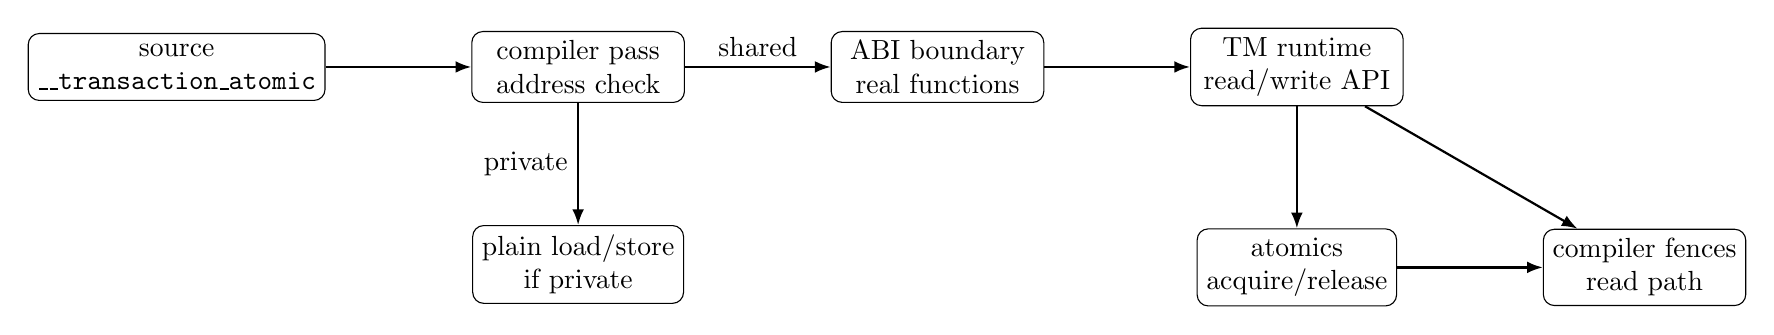
\begin{tikzpicture}[
    node distance=1.55cm and 1.85cm,
    box/.style={draw, rounded corners, align=center, minimum width=2.7cm, minimum height=0.85cm},
    small/.style={draw, rounded corners, align=center, minimum width=2.35cm, minimum height=0.75cm},
    arr/.style={-{Latex[length=2mm]}, thick}
]
\node[box] (src) {source\\\texttt{\_\_transaction\_atomic}};
\node[box, right=of src] (pass) {compiler pass\\address check};
\node[box, right=of pass] (abi) {ABI boundary\\real functions};
\node[box, right=of abi] (rt) {TM runtime\\read/write API};

\node[small, below=of pass] (plain) {plain load/store\\if private};
\node[small, below=of rt] (atoms) {atomics\\acquire/release};
\node[small, right=of atoms] (fence) {compiler fences\\read path};

\draw[arr] (src) -- (pass);
\draw[arr] (pass) -- node[above]{shared} (abi);
\draw[arr] (abi) -- (rt);
\draw[arr] (pass) -- node[left]{private} (plain);
\draw[arr] (rt) -- (atoms);
\draw[arr] (rt) -- (fence);
\draw[arr] (atoms) -- (fence);
\end{tikzpicture}%
}
\caption{A language-integrated TM boundary: the compiler decides which memory operations are instrumented; the runtime decides which atomics and fences implement the protocol.}
\label{fig:language-tm-boundary}
\end{figure}

\section{Language Integration Case Studies}
\subsection{Rust: The Borrow Checker and TM}
\begin{itemize}
    \item The borrow checker eliminates data races at compile time.
    \item \texttt{UnsafeCell} and interior mutability: what remains unprotected.
    \item How Rust’s safety guarantees can reduce (but not eliminate) the need for TM instrumentation.
    \item Rust's guarantees eliminate \emph{data races} but not \emph{deadlocks} or \emph{lost atomicity} --- the very guarantees TM adds on top of the language.
    \item \texttt{Sync}/\texttt{Send} traits as a way to reason about which values can be shared across threads; TM reifies ``shared mutable'' safety at runtime instead of compile time.
    \item The C++ and Rust stories are different in kind, not just degree: C++ gives the programmer \emph{control} over orderings; Rust removes whole classes of hazard at compile time. A TM layer must therefore integrate with each differently --- one C++ ABI, one Rust trait boundary.
\end{itemize}

\subsection{Language‑Integrated Annotations for TM}
\begin{itemize}
    \item GCC’s \texttt{\_\_transaction\_atomic} and \texttt{transaction\_safe} / \texttt{transaction\_pure} attributes.
    \item The (abandoned) C++ TM Technical Specification: transaction-safe functions, atomic blocks, and why the committee ultimately dropped it.
    \item Research proposals like \texttt{@atomic} blocks.
    \item This book's instrumentation plugin: a \texttt{[[tm::shared]]} annotation on globals, and the \texttt{LLVM\_TM\_ADDR\_CHECK} threshold deciding when instrumentation is actually needed.
    \item The three case studies (GCC, the C++ TS, this book's plugin) are a spectrum of how much the language commits to: the less the compiler enforces, the more the runtime must prove.
\end{itemize}

\begin{table}[htbp]
\centering
\begin{tabular}{p{0.21\textwidth}p{0.25\textwidth}p{0.25\textwidth}p{0.20\textwidth}}
\hline
Mechanism & Programmer contract & Runtime/compiler burden & Main hazard \\
\hline
\texttt{volatile} & Preserve visible accesses at compile time & Almost none & Not synchronization; CPU may reorder \\
C/C++ atomics & Choose ordering per operation & Implement the requested ordering & Correct but non-composable protocols \\
GCC atomic block & Mark transactional regions and safe calls & Compiler lowers loads, stores, and calls & Unsafe escape through non-transactional code \\
\texttt{[[tm::shared]]} plugin & Mark shared objects explicitly & Instrument only addresses that may alias shared state & Missed annotation loses atomicity \\
Rust trait boundary & Share only values satisfying \texttt{Send}/\texttt{Sync} contracts & Encapsulate mutation behind safe APIs or \texttt{UnsafeCell} & Interior mutability and FFI escape hatches \\
\hline
\end{tabular}
\caption{Language mechanisms differ in where they place the TM proof obligation.}
\label{tab:language-tm-taxonomy}
\end{table}

\section{Worked Example: Atomic Operations for a Counter}
\index{atomic operations}\index{C11 atomics}\index{volatile}\index{atomic\_signal\_fence}
\label{sec:atomics-example}

A shared counter is the smallest TM-relevant program. Compare the three
synchronisation styles on the same three lines of logic:

\begin{lstlisting}[language=C, caption={A shared counter three ways.}]
/* Locks: correct, coarse, non-composable. */
pthread_mutex_lock(&m); counter++; pthread_mutex_unlock(&m);

/* C11 atomics: fine-grained, but the orderings are on the programmer. */
int prev = atomic_fetch_add(&counter, 1, memory_order_relaxed);

/* TM: the block is the unit; orderings are the runtime's problem. */
__transaction_atomic { counter++; }
\end{lstlisting}

\begin{itemize}
    \item The atomic version exposes \emph{which} ordering to use per operation; the TM version hides the whole protocol.
    \item The TM runtime still needs the right atomics internally --- it just puts them behind one API (Part~IV).
    \item Composability reappears: two counters in one \texttt{atomic} block compose; two separate \texttt{atomic\_fetch\_add} calls do not.
    \item Exercise~3 of this chapter asks for the full C++ and Rust comparison.
\end{itemize}

\section{Worked Example: ABI-Safe Bank Transfer}
\index{ABI hazards}\index{compiler fence}\index{single global lock}\index{bank transfer}
\label{sec:abi-safe-bank-transfer}

The following example is deliberately an SGL-style TM. Its purpose is not
performance; it is the language boundary. The runtime exports functions, not
data symbols containing function pointers. The instrumented code calls those
functions and lets the runtime choose atomics and fences internally.

\begin{lstlisting}[language=C++, caption={A compilable C++ TM facade for the bank-transfer invariant.}]
#include <array>
#include <atomic>
#include <cassert>
#include <cstddef>

struct Account {
    int balance;
};

static std::array<Account, 2> bank{{Account{100}, Account{100}}};
static std::atomic_flag global_lock = ATOMIC_FLAG_INIT;

/* ABI boundary: real functions, not DATA symbols containing function pointers. */
extern "C" void tm_begin() {
    while (global_lock.test_and_set(std::memory_order_acquire)) {
        /* spin */
    }
}

extern "C" void tm_commit() {
    global_lock.clear(std::memory_order_release);
}

extern "C" int tm_read_i32(const int *p) {
    std::atomic_signal_fence(std::memory_order_seq_cst);
    int v = *p;
    std::atomic_signal_fence(std::memory_order_seq_cst);
    return v;
}

extern "C" void tm_write_i32(int *p, int v) {
    std::atomic_signal_fence(std::memory_order_seq_cst);
    *p = v;
    std::atomic_signal_fence(std::memory_order_seq_cst);
}

class TxGuard {
public:
    TxGuard() { tm_begin(); }
    ~TxGuard() { tm_commit(); }

    TxGuard(const TxGuard&) = delete;
    TxGuard& operator=(const TxGuard&) = delete;
};

static bool transfer(std::size_t from, std::size_t to, int amount, int floor) {
    TxGuard tx;

    int from_balance = tm_read_i32(&bank[from].balance);
    int to_balance = tm_read_i32(&bank[to].balance);

    if (from_balance - amount < floor) {
        return false;
    }

    tm_write_i32(&bank[from].balance, from_balance - amount);
    tm_write_i32(&bank[to].balance, to_balance + amount);
    return true;
}

static int total_money() {
    return bank[0].balance + bank[1].balance;
}

int main() {
    const int initial_total = total_money();

    assert(transfer(0, 1, 30, 0));
    assert(bank[0].balance >= 0);
    assert(bank[1].balance >= 0);
    assert(total_money() == initial_total);

    assert(!transfer(0, 1, 1000, 0));
    assert(total_money() == initial_total);
}
\end{lstlisting}

\begin{itemize}
    \item The acquire on \texttt{tm\_begin} and release on \texttt{tm\_commit} publish the critical section; the per-access fences only constrain the compiler.
    \item The source-level transaction is compositional: the floor check and both writes are one unit.
    \item The ABI contract is visible: instrumented code calls \texttt{tm\_read\_i32} and \texttt{tm\_write\_i32}; non-instrumented code must not bypass shared state.
    \item This is the semantic baseline implemented by SGL and TSX-SGL before more selective protocols such as NOrec, TL2, and TSC-TM reduce contention.
\end{itemize}

\section{Worked Example: Model Checking Lost Atomicity}
\index{TLA+}\index{lost atomicity}\index{money conservation}
\label{sec:tla-bank-language-contract}

Language support for TM should preserve the same invariant as the runtime:
the transfer either commits as one state transition or has no effect. A small
TLA+ model captures that contract without mentioning cache lines, fences, or
calling conventions.

\begin{lstlisting}[language={}, caption={A TLC-checkable TLA+ model of an atomic bank transfer.}]
---- MODULE BankTMAtomicity ----
EXTENDS Naturals

A0 == 10
A1 == 10
Floor == 0
Amount == 3

VARIABLES bal, pc

vars == <<bal, pc>>

Init ==
    /\ bal = [0 |-> A0, 1 |-> A1]
    /\ pc = "idle"

CanTransfer ==
    bal[0] >= Amount + Floor

Begin ==
    /\ pc = "idle"
    /\ pc' = "active"
    /\ UNCHANGED bal

Commit ==
    /\ pc = "active"
    /\ CanTransfer
    /\ bal' = [bal EXCEPT ![0] = @ - Amount,
                          ![1] = @ + Amount]
    /\ pc' = "idle"

Abort ==
    /\ pc = "active"
    /\ ~CanTransfer
    /\ pc' = "idle"
    /\ UNCHANGED bal

Idle ==
    /\ pc = "idle"
    /\ UNCHANGED vars

Next ==
    Begin \/ Commit \/ Abort \/ Idle

Spec ==
    Init /\ [][Next]_vars

InvMoney ==
    bal[0] + bal[1] = A0 + A1

InvFloor ==
    bal[0] >= Floor /\ bal[1] >= Floor

THEOREM Spec => []InvMoney
THEOREM Spec => []InvFloor
====
\end{lstlisting}

\begin{itemize}
    \item The model treats the transaction body as one commit transition; this is the property language integration must preserve.
    \item \texttt{InvMoney} catches partial instrumentation: debiting without crediting violates conservation.
    \item \texttt{InvFloor} catches a misplaced check: the account floor must be tested in the same atomic unit as the debit.
    \item The model abstracts away C++ and Rust details; those details re-enter at the ABI and trait boundaries.
\end{itemize}

\section{Summary}
\begin{itemize}
    \item Different languages offer different levels of memory‑ordering control.
    \item A type system that prevents data races still cannot enforce atomicity across multiple memory locations without TM support.
\end{itemize}

\section{Exercises}
\begin{enumerate}
    \item In C, a compiler hoists a read of \texttt{x} out of an \texttt{atomic} block. Explain how \texttt{volatile} or an \texttt{asm} barrier can prevent this, and what the runtime cost is.
    \item A Rust program uses \texttt{RefCell}. Explain why an STM that instruments all loads and stores still cannot protect against a data race without additional runtime checks.
    \item Compare the programming effort required to add a thread-safe counter using locks, atomics, and a TM in C++ and Rust.
    \item \emph{[implementation]} Extend the ABI-safe bank-transfer example with a second shared object, \texttt{transfer\_count}. Update it inside the same transaction as the two account balances. Then write a non-transactional version using three separate atomics and identify an interleaving that preserves each individual atomic operation but violates the intended compound invariant.
    \item \emph{[verification]} Modify the TLA+ model in the lost-atomicity example by splitting \texttt{Commit} into two transitions, one debit and one credit. Run TLC on the finite model and record the shortest counterexample to \texttt{InvMoney}. Explain which source-level compiler or ABI mistake the split transition represents.
    \item \emph{[theory]} Compare a C++ TM API based on explicit \texttt{std::memory\_order} parameters with a Rust API based on a \texttt{TxCell<T>} wrapper. For each API, state what the type system proves, what the runtime must still validate, and where unsafe escape hatches can break atomicity.
\end{enumerate}

% -------------------------------------------------------------------
%  PART III: FORMAL FOUNDATIONS: MATHEMATICS AND VERIFICATION
% -------------------------------------------------------------------
\part{Formal Foundations: Mathematics and Verification}

\chapter{Mathematical Foundations}
\section{Automata and Formal Languages}
\begin{itemize}
    \item Finite automata (DFA/NFA) and regular expressions.
    \item Context-free grammars --- tie back to recursive descent.
    \item Used for real in Chapter~15: the DFA in Figure~\ref{fig:lexer-dfa} is the lexer's recognizer, and the LR(0) automaton in Figure~\ref{fig:lr0-automaton} is the shift-reduce table that Bison-family generators build from a grammar.
\end{itemize}

\section{Markov Chains}
\begin{itemize}
    \item Discrete-time Markov chains (DTMC): states, transition matrices, steady-state probabilities.
    \item Modeling a transaction's lifecycle: Active, Validating, Aborted, Committed.

\begin{figure}[ht]
\centering
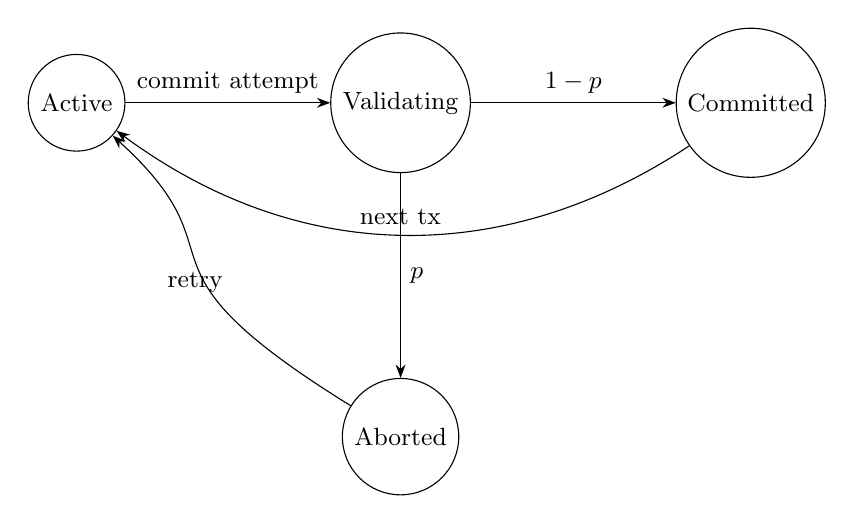
\begin{tikzpicture}[node distance=2.6cm, font=\small]
  \node[draw,circle,minimum size=1.1cm] (active) {Active};
  \node[draw,circle,minimum size=1.1cm] (valid) [right=of active] {Validating};
  \node[draw,circle,minimum size=1.1cm] (committed) [right=of valid] {Committed};
  \node[draw,circle,minimum size=1.1cm] (aborted) [below=of valid] {Aborted};
  \draw[-{Stealth}] (active) -- node[above] {commit attempt} (valid);
  \draw[-{Stealth}] (valid) -- node[above] {$1-p$} (committed);
  \draw[-{Stealth}] (valid) -- node[right] {$p$} (aborted);
  \draw[-{Stealth}] (aborted) .. controls (0.5,-2) and (2.2,-2) .. node[below] {retry} (active);
  \draw[-{Stealth}] (committed) to[bend left=35] node[above] {next tx} (active);
\end{tikzpicture}
\caption{The transaction lifecycle as a Markov chain: a commit attempt either succeeds or aborts, and an abort re-enters the active state.}
\label{fig:tx-lifecycle}
\end{figure}

    \item The key modeling assumption: memoryless transitions, and when that assumption is reasonable for abort/retry loops.
    \item Expected number of retries before a successful commit as a function of abort probability; closed-form via the geometric distribution.
    \item Continuous-time counterpart, CTMC and queueing, used in Part~VI for throughput prediction.
    \item The model's \emph{purpose} in the book: give every later chapter a number where it can get one, and hand off where it cannot. Data-dependent contention belongs to Part~III's model checking.
\end{itemize}

If a commit attempt aborts with probability

$$
p
$$

and succeeds with probability

$$
1-p
$$

then the expected number of attempts per committed transaction is

$$
E[\mathrm{attempts}] = \frac{1}{1-p}.
$$

\section{Queueing Theory and Little's Law}
\begin{itemize}
    \item Basic notions: arrival rate, average service time, and average number in the system.
    \item Applying Little's Law to a transactional system to estimate congestion.
    \item Little's Law:

$$
L = \lambda S
$$

where

$$
L
$$

is the average number of in-flight transactions,

$$
\lambda
$$

is the committed throughput, and

$$
S
$$

is the average residence time.

    \item Throughput falls when retries inflate the effective service time.
    \item The ``wasted-work'' multiplier is the retry series:

$$
\sum_{i=0}^{\infty} p_{\mathrm{abort}}^i
  =
\frac{1}{1-p_{\mathrm{abort}}}.
$$

    \item Where the models break: contention is data-dependent and non-Poisson, which is exactly why Part~III's model checking complements the analysis.
\end{itemize}

\begin{table}[htbp]
\centering
\begin{tabular}{p{0.16\linewidth}p{0.18\linewidth}p{0.30\linewidth}p{0.26\linewidth}}
\hline
Tool & Object modeled & Question answered & Typical TM use \\
\hline
DFA / grammar & Program text & Is this input syntactically valid? & Lexer and parser construction \\
DTMC & Transaction lifecycle & How many retries should we expect? & Abort and retry estimates \\
Little's Law & Queue of transactions & How many transactions are in flight? & Congestion and saturation estimates \\
Model checking & Reachable executions & Can this bad state occur? & Safety invariants and races \\
\hline
\end{tabular}
\caption{The mathematical tools used in the book. Analytical models estimate cost; model checking explores executions.}
\label{tab:math-tools}
\end{table}

\section{Worked Example: Numbers, Not Just Symbols}
\index{geometric distribution}\index{Little's Law}\index{Markov chain}
\label{sec:math-example}

The geometric retry model, populated with a few abort probabilities. If a
transaction aborts with probability

$$
p
$$

and retries until it commits, the number of attempts follows a geometric distribution with mean

$$
\frac{1}{1-p}.
$$

\begin{lstlisting}[caption={The geometric retry model, numerically.}]
p        E[attempts] = 1/(1-p)     P(commits within 5 tries)
0.10     1.11                      0.99999
0.50     2.00                      0.96875
0.90     10.0                      0.40951
\end{lstlisting}

\begin{itemize}
    \item The ``wasted-work'' multiplier of this section is exactly the expected number of attempts.
    \item At an abort probability of

$$
0.90
$$

every committed transaction performs ten attempts on average.

    \item Plug into Little's Law by replacing service time with effective service time:

$$
S_{\mathrm{effective}} = \frac{S}{1-p}.
$$

    \item The same probability feeds the Markov chain of Exercise~1, and the model-checking exercises of Part~III inject the corresponding state transitions.
\end{itemize}

\section{Worked Example: Simulating Retry Cost in the Bank}
\index{bank transfer}\index{abort probability}\index{money conservation}
\label{sec:math-bank-simulation}

The next program is deliberately not a TM implementation. It is the mathematical model made executable: a bank transfer retries until the synthetic validator accepts the commit attempt. The committed state must still satisfy the account floor and money-conservation invariant.

\begin{lstlisting}[language=C++, caption={A compilable C++17 simulation of geometric retry cost for bank transfers.}]
#include <cassert>
#include <cstdint>
#include <iostream>
#include <random>
#include <stdexcept>
#include <vector>

struct Bank {
    std::vector<long long> bal;
    long long floor;
};

static long long total(const Bank& b) {
    long long s = 0;
    for (long long x : b.bal) s += x;
    return s;
}

static bool invariant_holds(const Bank& b, long long initial_total) {
    if (total(b) != initial_total) return false;
    for (long long x : b.bal) {
        if (x < b.floor) return false;
    }
    return true;
}

static int transfer_with_retries(Bank& b,
                                 int from,
                                 int to,
                                 long long amount,
                                 double abort_probability,
                                 std::mt19937_64& rng) {
    if (from == to) throw std::invalid_argument("self-transfer");
    if (amount < 0) throw std::invalid_argument("negative amount");

    std::bernoulli_distribution aborts(abort_probability);
    int attempts = 0;

    for (;;) {
        ++attempts;

        const long long src = b.bal.at(from);
        const long long dst = b.bal.at(to);

        if (src - amount < b.floor) {
            return attempts; // transaction is rejected, not committed
        }

        if (aborts(rng)) {
            continue;        // validation failed; retry same transaction
        }

        b.bal.at(from) = src - amount;
        b.bal.at(to)   = dst + amount;
        return attempts;
    }
}

int main() {
    Bank b{{1000, 1000}, 0};
    const long long initial_total = total(b);

    std::mt19937_64 rng(7);
    const double p_abort = 0.50;

    long long attempts = 0;
    long long committed = 0;

    for (int i = 0; i < 10000; ++i) {
        attempts += transfer_with_retries(b, 0, 1, 1, p_abort, rng);
        ++committed;
        assert(invariant_holds(b, initial_total));
    }

    std::cout << "committed=" << committed
              << " attempts=" << attempts
              << " mean_attempts="
              << static_cast<double>(attempts) / committed
              << "\n";
}
\end{lstlisting}

\begin{itemize}
    \item The simulation separates safety from performance: retries change the number of attempts, not the invariant.
    \item The account floor is checked before the write set is installed.
    \item The expected mean attempts approach the geometric value as the number of transfers grows.
    \item Real backends replace the synthetic Bernoulli validator with concrete validation mechanisms: NOrec validates a value-based read set, TL2 validates versions, and MV designs validate snapshots.
\end{itemize}

\begin{figure}[htbp]
\centering
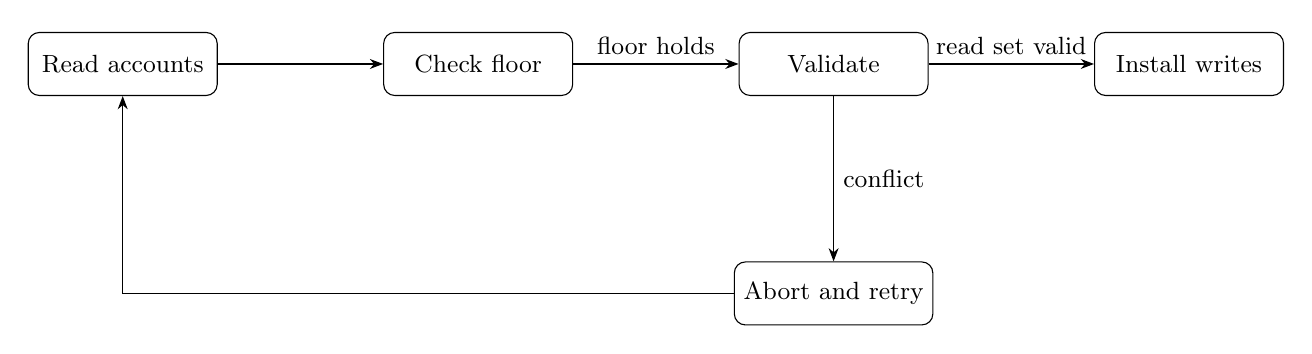
\begin{tikzpicture}[node distance=2.1cm, font=\small]
  \node[draw,rounded corners,minimum width=2.4cm,minimum height=0.8cm] (read) {Read accounts};
  \node[draw,rounded corners,minimum width=2.4cm,minimum height=0.8cm,right=of read] (check) {Check floor};
  \node[draw,rounded corners,minimum width=2.4cm,minimum height=0.8cm,right=of check] (validate) {Validate};
  \node[draw,rounded corners,minimum width=2.4cm,minimum height=0.8cm,right=of validate] (install) {Install writes};
  \node[draw,rounded corners,minimum width=2.4cm,minimum height=0.8cm,below=of validate] (abort) {Abort and retry};

  \draw[-{Stealth}] (read) -- (check);
  \draw[-{Stealth}] (check) -- node[above] {floor holds} (validate);
  \draw[-{Stealth}] (validate) -- node[above] {read set valid} (install);
  \draw[-{Stealth}] (validate) -- node[right] {conflict} (abort);
  \draw[-{Stealth}] (abort) -| ($(read.south)+(0,-0.4)$) -- (read.south);
\end{tikzpicture}
\caption{A bank transaction as a validation pipeline. Analytical models collapse the conflict edge into an abort probability; model checking keeps the states explicit.}
\label{fig:bank-validation-pipeline}
\end{figure}

\section{Worked Example: Model Checking Money Conservation}
\index{TLA+}\index{model checking}\index{invariant}
\label{sec:math-bank-tla}

The same bank example can be written as a finite-state TLA+ model. TLC checks all reachable states for the two invariants used throughout the book: money is conserved and every account remains above the floor.

\begin{lstlisting}[caption={A model-checkable TLA+ specification for a two-account transfer.}]
---- MODULE BankInvariant ----
EXTENDS Integers, TLC

Accounts == {0, 1}
InitBal == [a \in Accounts |-> 10]
Amount == 3
Floor == 0

VARIABLES bal, phase, snap

Vars == <<bal, phase, snap>>

Init ==
    /\ bal = InitBal
    /\ snap = InitBal
    /\ phase = "idle"

Begin ==
    /\ phase = "idle"
    /\ snap' = bal
    /\ phase' = "read"
    /\ UNCHANGED bal

Commit ==
    /\ phase = "read"
    /\ snap[0] - Amount >= Floor
    /\ bal' = [bal EXCEPT ![0] = snap[0] - Amount,
                          ![1] = snap[1] + Amount]
    /\ phase' = "idle"
    /\ UNCHANGED snap

Abort ==
    /\ phase = "read"
    /\ snap[0] - Amount < Floor
    /\ phase' = "idle"
    /\ UNCHANGED <<bal, snap>>

Next == Begin \/ Commit \/ Abort

Spec == Init /\ [][Next]_Vars

MoneyConserved ==
    bal[0] + bal[1] = InitBal[0] + InitBal[1]

AccountFloors ==
    \A a \in Accounts : bal[a] >= Floor

Inv == MoneyConserved /\ AccountFloors

THEOREM Spec => []Inv
====
\end{lstlisting}

\begin{itemize}
    \item The specification is small because the state space is small: two accounts, one transfer amount, one transaction phase variable.
    \item The invariant is independent of the retry policy. Retry affects liveness and cost; the checked predicate is safety.
    \item The theorem line states the same obligation enforced by the C++ assertion in \S\ref{sec:math-bank-simulation}.
    \item Larger TLA+ models in the companion project use the same discipline: explicit state, explicit transition relation, explicit invariant.
\end{itemize}

\section{Summary}
\begin{itemize}
    \item Formal languages underpin compiler construction.
    \item Markov chains and queueing theory provide first-order performance models for TM.
    \item Analytical models predict; model checking proves; the two tools answer different questions.
\end{itemize}

\section{Exercises}
\begin{enumerate}
    \item Build a three-state Markov chain for a transaction under contention and compute the expected number of retries before a successful commit.
    \item In a TM system with arrival rate

$$
\lambda
$$

and average transaction length

$$
T
$$

use Little's Law to estimate the effect on the number of in-flight transactions when the abort rate doubles.

    \item Model a TM that retries after a random back-off as a Markov chain and determine the back-off probability that maximizes throughput.
    \item \emph{[implementation]} Extend the simulation in \S\ref{sec:math-bank-simulation} to choose the source and destination accounts uniformly at random. Keep the money-conservation assertion and report the measured mean attempts for abort probabilities

$$
0.10,\quad 0.50,\quad 0.90.
$$

    \item \emph{[verification]} Modify the TLA+ model in \S\ref{sec:math-bank-tla} so that an abort may occur nondeterministically even when the floor check succeeds. Check that the invariant still holds.
    \item \emph{[theory]} Derive the expected attempts per committed transaction when a transaction has two independent validation phases with abort probabilities

$$
p_1
$$

and

$$
p_2.
$$

State clearly whether the result changes if the two validation phases are correlated.
\end{enumerate}


\chapter{Formal Design with PlusCal and TLA+}
\section{TLA+ and PlusCal in a Nutshell}
\begin{itemize}
    \item State machines, variables, actions.
    \item PlusCal syntax: labels, \texttt{either/or}, \texttt{assert}, invariants.
    \item Safety (bad states never occur) vs.\ liveness (good states eventually occur) --- the two obligations a TM model must state separately.
    \item Why a model is a design tool, not just a proof tool: the act of writing the model forces the empty corner cases into view.
\end{itemize}

\section{Specifying and Checking Simple TM Algorithms}
\begin{itemize}
    \item Single‑global‑lock TM in PlusCal.
    \item NOrec (value‑based validation, timestamp‑based writes) in PlusCal.
    \item Translating PlusCal to TLA+ and running TLC.
    \item The companion repository contains checked models for every backend in this book: SGL, TL2, NOrec, TinySTM variants, MVLog, JVSTM, plus GPU models (PR-STM, JVSTM, GUST) at warp granularity.
    \item Invariants that matter: opacity/reduced order, lock exclusion, commit-clock monotonicity, ``no committed transaction can be invalidated.''
    \item TLC as an oracle that catches the ``obviously correct'' bug --- e.g.\ the read-validate\slash{}snapshot-threshold bugs discussed in Part~IV and Part~VII.
\end{itemize}

\begin{table}[htbp]
\centering
\small
\begin{tabular}{p{0.15\linewidth}p{0.21\linewidth}p{0.28\linewidth}p{0.26\linewidth}}
\hline
\textbf{Design family} & \textbf{Representative backend} & \textbf{Modelled shared state} & \textbf{Main safety check} \\
\hline
Serial lock & SGL, PersistentSGL & lock bit, heap & mutual exclusion, opacity \\
Value validation & NOrec, NOrec-BF & sequence clock, read values & stale read rejection \\
Versioned locks & TL2, TSC-TM & orecs, versions, ownership & lock/version consistency \\
Undo/redo STM & TinySTM variants & ownership, write sets & ownership before write-back \\
Multi-version & JVSTM, MVLog & versions, commit order & visible snapshot consistency \\
GPU commit-log & GUST & log, CCT, MRV tables & no missed conflict \\
Distributed 2PC & TiKV/Percolator & locks, writes, timestamps & atomic visibility \\
\hline
\end{tabular}
\caption{A small taxonomy of what the model must remember. The runtime code may contain allocators, barriers, persistence fences, or RPCs; the model keeps only the state needed to falsify the advertised TM property.}
\label{tab:tla-taxonomy}
\end{table}

\section{Worked Example: A Single-Global-Lock TM in PlusCal}
\index{PlusCal}\index{TLA+}\index{TLC}\index{invariant}\index{model checking}\index{counterexample}\index{liveness}
\label{sec:pluscal-example}

The simplest TM in this book, in the notation that Chapter~6's invariants
check.  Figure~\ref{fig:pluscal-latex} shows the same algorithm twice:
once as the PlusCal source that is model-checked (left), and once as the
pseudo-code that \textsc{TLATeX} (\texttt{tla2tex.TLA}) typesets from that
same source (right).  This is the point of PlusCal: the algorithm in a
paper and the specification checked by TLC are \emph{the same text}.

\begin{figure}[ht]
\centering
\begin{minipage}[t]{0.47\textwidth}
\centering\textbf{(a) PlusCal source}\\[2pt]
\begin{lstlisting}[basicstyle=\ttfamily\footnotesize]
--algorithm sgl
variables lock = FALSE, x = 0, y = 0;
process Tx \in 1..2
variables rs = {}, ws = {};
begin
  begin_tx:
    await lock = FALSE; lock := TRUE;
  body:
    rs := rs \cup {x, y};          (* reads *)
    ws := ws \cup {x, y};          (* writes *)
  commit:
    x := 2; y := 2;                (* write-back *)
    lock := FALSE;
end process
\end{lstlisting}
\end{minipage}\hfill
\begin{minipage}[t]{0.47\textwidth}
\centering\textbf{(b) \textsc{TLATeX} pseudo-code output}\\[2pt]
{\footnotesize
\begin{tabbing}
  \hspace{0.9cm}\=\hspace{3.1cm}\=\hspace{2.6cm}\=\hspace{2.5cm}\=\kill
  \textbf{--algorithm} \emph{sgl} \\
  \textbf{variables} \> \texttt{lock = FALSE, x = 0, y = 0}; \\
  \textbf{process} \> \texttt{Tx in 1..2} \\
  \> \textbf{variables} \> \texttt{rs = \{\}, ws = \{\}}; \\
  \textbf{begin} \\
  \> \texttt{begin\_tx:} \\
  \> \> \textbf{await} \> \texttt{lock = FALSE}; \texttt{lock := TRUE}; \\
  \> \texttt{body:} \\
  \> \> \texttt{rs := rs union \{x, y\}}; \> \> reads \\
  \> \> \texttt{ws := ws union \{x, y\}}; \> \> writes \\
  \> \texttt{commit:} \\
  \> \> \texttt{x := 2; y := 2}; \> \> write-back \\
  \> \> \texttt{lock := FALSE}; \\
  \textbf{end process}
\end{tabbing}
}
\end{minipage}
\caption{A single-global-lock TM, twice. (a) is the PlusCal source kept in the repository and model-checked with TLC; (b) is the pseudo-code that \textsc{TLATeX} produces from the \emph{same} file --- the paper figure can never drift from the verified algorithm.}
\label{fig:pluscal-latex}
\end{figure}

\begin{itemize}
    \item Every invariant of this chapter is trivially true here --- the lock serialises everything --- which is exactly why SGL is the reference design every optimistic backend is checked against.
    \item The companion repository's \texttt{SGL.tla} is this model plus the opacity invariant, and it passes TLC.
    \item Exercise~1 asks you to add read-set validation to this model; the point is that even this ``obviously correct'' design needs the check spelled out.
    \item Contrast with the optimistic designs of Part~IV: the moment the lock disappears, the invariants become non-trivial and TLC earns its keep.
\end{itemize}

\section{Bug‑Injection and Counterexample Analysis}
\begin{itemize}
    \item Deliberately omitting a read‑set validation.
    \item Reading the TLC counterexample trace to localise the bug.
    \item Mutation testing for models: remove the guard, remove the fence, remove the re-validation, and confirm TLC finds each injected bug.
    \item Counterexamples vs.\ crashes: a TLC trace before an invariant violation is a precise, replayable schedule --- exactly the artifact a debugger cannot easily produce for real runs.
\end{itemize}

\section{Worked Example: Bank Transfer Under a Single Global Lock}
\index{bank transfer}\index{single global lock}\index{PlusCal}

The running bank example is a two-account transfer.  The model is intentionally
small: two accounts, two transactions, one unit transferred from account~1 to
account~2.  The interesting part is not the arithmetic; it is that the floor
and conservation checks are written at the same point where the runtime would
return success to the caller.

\begin{lstlisting}[caption={A complete PlusCal model of the bank transfer under SGL.}]
---- MODULE BankSGL ----
EXTENDS Naturals, TLC

Accounts == 1..2
Initial == [a \in Accounts |-> 10]
Total(b) == b[1] + b[2]

(*--algorithm BankSGL
variables
  lock = FALSE,
  bal = Initial,
  committed = [t \in 1..2 |-> FALSE];

process Tx \in 1..2
variables
  from = 1,
  to = 2,
  amount = 1,
  seen = 0;
begin
BeginTx:
  await lock = FALSE;
  lock := TRUE;

Read:
  seen := bal[from];

WriteBack:
  if seen >= amount then
    bal[from] := bal[from] - amount;
    bal[to] := bal[to] + amount;
    committed[self] := TRUE;
  end if;

Check:
  assert Total(bal) = 20;
  assert bal[1] >= 0 /\ bal[2] >= 0;

Commit:
  lock := FALSE;
end process;
end algorithm; *)
====
\end{lstlisting}

\begin{itemize}
    \item The invariant is checked after write-back, not only at initialization.
    \item The lock makes the state space small enough that TLC explores all interleavings of both transactions.
    \item The model does not claim performance.  It claims that every checked execution preserves the account floors and total money.
    \item SGL is a useful reference because every optimistic backend should refine the same externally visible transfer behavior.
\end{itemize}

\section{Worked Example: NOrec-Style Validation for the Bank}
\index{NOrec}\index{validation}\index{opacity}\index{read set}

NOrec replaces ownership metadata with a global sequence clock and value-based
validation.  A reader records a snapshot and the values it observed.  If the
clock changes before commit, the read values must still match memory; otherwise
the transaction aborts.  The following model is deliberately finite and omits
allocation, privatization, and signal recovery.  It is the core validation
discipline.

\begin{lstlisting}[caption={A finite PlusCal model of NOrec-style value validation.}]
---- MODULE BankNOrecValue ----
EXTENDS Naturals, TLC

Accounts == 1..2
Initial == [a \in Accounts |-> 10]
Total(b) == b[1] + b[2]

(*--algorithm BankNOrecValue
variables
  commitLock = FALSE,
  clock = 0,
  bal = Initial;

process Tx \in 1..2
variables
  snap = 0,
  r1 = 0,
  r2 = 0,
  amount = 1,
  ok = FALSE;
begin
BeginTx:
  snap := clock;

Read1:
  r1 := bal[1];

Read2:
  r2 := bal[2];

Validate:
  if clock = snap then
    ok := TRUE;
  else
    ok := (r1 = bal[1] /\ r2 = bal[2]);
  end if;

Commit:
  if ok /\ r1 >= amount then
    await commitLock = FALSE;
    commitLock := TRUE;

    if clock = snap /\ r1 = bal[1] /\ r2 = bal[2] then
      bal[1] := bal[1] - amount;
      bal[2] := bal[2] + amount;
      clock := clock + 1;
    end if;

    assert Total(bal) = 20;
    assert bal[1] >= 0 /\ bal[2] >= 0;

    commitLock := FALSE;
  end if;
end process;
end algorithm; *)
====
\end{lstlisting}

\begin{itemize}
    \item The first validation is a fast path: if the clock did not change, the read set is still valid.
    \item The second validation is the commit-time defense.  Removing it is a standard bug-injection test.
    \item Value validation compares the values read, not only the timestamp.  This is the point that distinguishes NOrec from a naive global-clock scheme.
    \item The model is small, but it captures the critical opacity question: no transaction may commit after observing a mixed snapshot.
\end{itemize}

\begin{figure}[htbp]
\centering
\resizebox{\textwidth}{!}{%
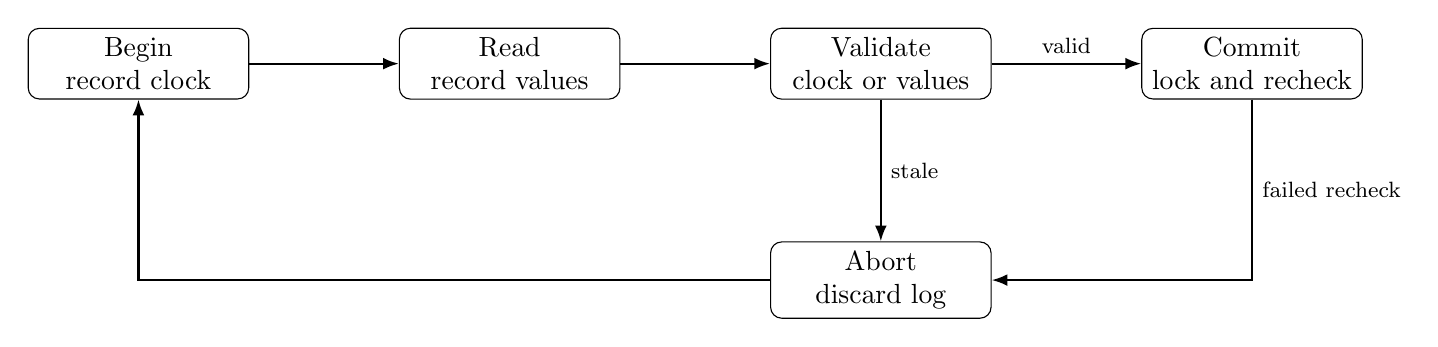
\begin{tikzpicture}[
    node distance=1.8cm and 1.9cm,
    state/.style={draw, rounded corners, minimum width=2.8cm, minimum height=0.85cm, align=center},
    edge/.style={-{Latex[length=2mm]}, thick}
]
\node[state] (begin) {Begin\\record clock};
\node[state, right=of begin] (read) {Read\\record values};
\node[state, right=of read] (validate) {Validate\\clock or values};
\node[state, right=of validate] (commit) {Commit\\lock and recheck};
\node[state, below=of validate] (abort) {Abort\\discard log};

\draw[edge] (begin) -- (read);
\draw[edge] (read) -- (validate);
\draw[edge] (validate) -- node[above, font=\footnotesize]{valid} (commit);
\draw[edge] (validate) -- node[right, font=\footnotesize]{stale} (abort);
\draw[edge] (commit) |- node[pos=0.25, right, font=\footnotesize]{failed recheck} (abort);
\draw[edge] (abort) -| ($(begin.south)+(0,-0.4)$) -- (begin.south);
\end{tikzpicture}%
}
\caption{Validation state machine for the finite NOrec-style model. TLC explores all interleavings through these states; the useful counterexamples are usually the paths where validation succeeds too early or commit omits the final recheck.}
\label{fig:norec-validation-sm}
\end{figure}

\section{The Complete Verification Workflow}
\label{sec:verify-workflow}
What ``we checked this with TLC'' means, end to end, so the claim is
reproducible rather than rhetorical:

\begin{enumerate}
    \item \textbf{Specify} the algorithm in PlusCal (a \texttt{--algorithm} block), with the correctness condition encoded as invariants (e.g.\ opacity via \texttt{InvNoMissedConflict}).
    \item \textbf{Add temporal properties} where liveness matters (a committed-transaction progress property under weak fairness).
    \item \textbf{Configure TLC}: a \texttt{.cfg} listing the model constants, the invariant, the optional \texttt{PROPERTY}, and a state bound so the checker terminates.
    \item \textbf{Run} \texttt{tlc} and read the state-count line --- \emph{how much} of the state space was explored matters as much as the absence of errors.
    \item \textbf{Inject a bug} (Section ``Bug-Injection'') and confirm the checker finds it: a test of a model that never fails is a test of the model's triviality.
    \item \textbf{Document the limits}: bounded state spaces and abstraction gaps (no call stack, no jmp-buffer lifetime) are what the model cannot see.
\end{enumerate}

\begin{table}[ht]
\centering
\small
\begin{tabular}{llll}
\hline
\textbf{Runtime (Part IV/VII)} & \textbf{TLA+ model} & \textbf{Key invariant} & \textbf{Result} \\
\hline
SGL (Ch.~8)     & \texttt{SGL.tla}         & opacity (all invariants) & TLC pass \\
NOrec (Ch.~9)   & \texttt{NOrec.tla}       & value-validation opacity  & TLC pass \\
TL2 (Ch.~9)     & \texttt{TL2.tla}         & versioned-lock correctness & TLC pass \\
TinySTM (Ch.~9) & \texttt{TinySTM\_WBCTL.tla} & lock/ownership invariants & TLC pass \\
Romulus (Ch.~9) & \texttt{Romulus.tla}     & read-validate OCC          & TLC pass \\
GPU GUST (Ch.~17)& \texttt{GPU\_GUST.tla}  & \texttt{InvNoMissedConflict} & TLC pass \\
\hline
\end{tabular}
\caption{Runtime-to-model traceability in the companion repository: every chapter that introduces a runtime names the PlusCal/TLA+ file, the invariant checked, and the outcome. The repository's \texttt{docs/proofs} directory is the source of truth; this table is its index.}
\label{tab:traceability}
\end{table}

\begin{itemize}
    \item The workflow is the connective tissue between Part~III (formalism) and Part~IV (runtimes): a backend ``is verified'' only in the sense of steps 1--6 above.
    \item Figure~\ref{fig:pluscal-latex} is step~1's artifact: the same source that TLC checks is the figure a reader sees.
    \item Figure~\ref{fig:norec-validation-sm} is the corresponding artifact for optimistic validation: it names the states where injected bugs should be placed.
\end{itemize}

\section{Summary}
\begin{itemize}
    \item Model checking provides formal guarantees about TM algorithm correctness.
    \item Even simple TM designs can harbour subtle bugs that TLC exposes.
    \item The model is not the implementation.  It is the executable argument that the implementation's concurrency protocol has the advertised shape.
    \item The useful models are small, finite, and hostile: they should make wrong interleavings easy for TLC to find.
\end{itemize}

\section{Exercises}
\begin{enumerate}
    \item Extend the single‑global‑lock PlusCal model with an explicit read‑set validation step. Use TLC to check that opacity holds.
    \item The NOrec model can fail if it uses only timestamp validation without value‑based validation. Insert this bug and show the TLC output that reveals it.
    \item Specify a TM that uses eager locking and use TLC to find a deadlock scenario.
    \item \emph{[implementation]} Add a tiny C++ harness that runs the bank transfer under the repository's SGL and NOrec backends with two worker threads. Check the same two runtime assertions used in the models: total money is conserved and no account falls below its floor.
    \item \emph{[verification]} Mutate the protocol of Figure~\ref{fig:norec-validation-sm} by removing the commit-time recheck from \texttt{BankNOrecValue}. State the invariant that fails and summarize the shortest TLC counterexample trace.
    \item \emph{[theory]} Explain why lock exclusion alone is insufficient for opacity in an optimistic STM. Give a two-transaction history with a stale read, then identify which validation edge in Figure~\ref{fig:norec-validation-sm} must reject it.
\end{enumerate}


% -------------------------------------------------------------------
%  PART IV: IMPLEMENTING TRANSACTIONAL MEMORY
% -------------------------------------------------------------------
\part{Implementing Transactional Memory}

\chapter{Transaction API Design – Software Engineering Perspectives}
\section{Classic Synchronous API}
\begin{itemize}
    \item \texttt{tm\_begin()}, \texttt{tm\_read()}, \texttt{tm\_write()}, \texttt{tm\_commit()}, \texttt{tm\_abort()}.
    \item Thread‑local transaction descriptors and the need for thread‑entry instrumentation.
    \item Typed wrappers (\texttt{tm\_read\_i4}, \texttt{tm\_write\_i4}, \ldots) and how they map onto the byte-oriented core.
    \item The retry loop: \texttt{sigsetjmp}/\texttt{siglongjmp} (or equivalent) to restart aborted transactions --- and the frame-lifetime hazard this creates (Part~VI).
    \item The set of primitives is deliberately small; everything else (nested transactions, retry, allocation) is built on top.
\end{itemize}

\begin{figure}[htbp]
\centering
\resizebox{\textwidth}{!}{%
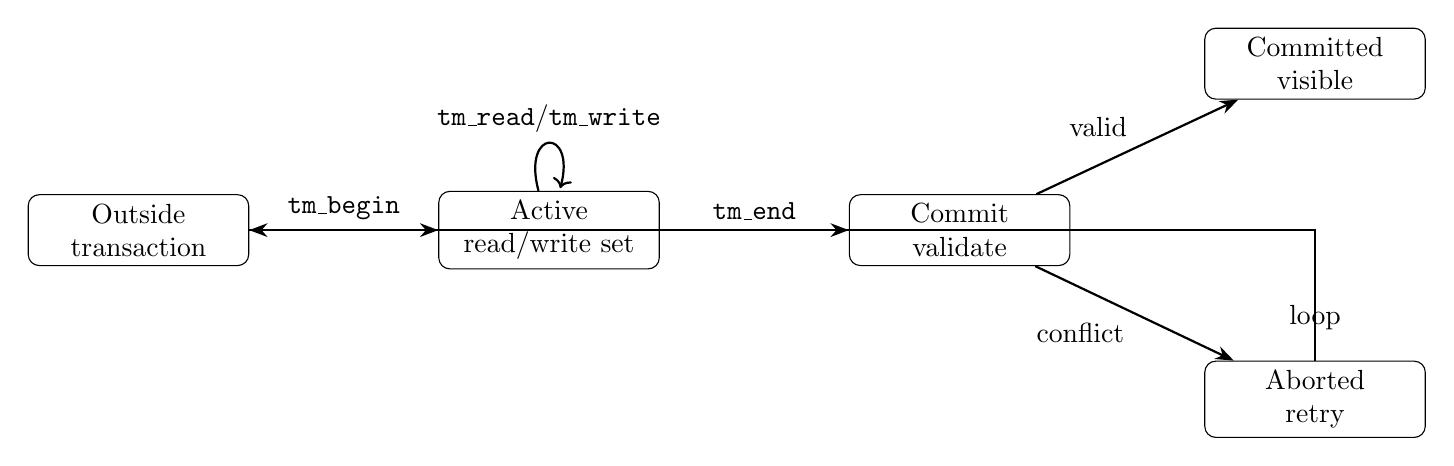
\begin{tikzpicture}[
    node distance=1.8cm and 2.4cm,
    state/.style={draw, rounded corners, minimum width=2.8cm, minimum height=0.9cm, align=center},
    arrow/.style={-{Stealth}, thick}
]
\node[state] (outside) {Outside\\transaction};
\node[state, right=of outside] (active) {Active\\read/write set};
\node[state, right=of active] (commit) {Commit\\validate};
\node[state, above right=1.2cm and 1.7cm of commit] (done) {Committed\\visible};
\node[state, below right=1.2cm and 1.7cm of commit] (retry) {Aborted\\retry};

\draw[arrow] (outside) -- node[above]{\texttt{tm\_begin}} (active);
\draw[arrow] (active) edge[loop above] node{\texttt{tm\_read}/\texttt{tm\_write}} (active);
\draw[arrow] (active) -- node[above]{\texttt{tm\_end}} (commit);
\draw[arrow] (commit) -- node[above left]{valid} (done);
\draw[arrow] (commit) -- node[below left]{conflict} (retry);
\draw[arrow] (retry) |- node[pos=0.25, below]{loop} (outside);
\end{tikzpicture}%
}
\caption{Control states exposed by the synchronous transaction API. Backends differ in validation and metadata, but the source-level protocol is the same.}
\label{fig:api-state-machine}
\end{figure}

\section{Worked Example: The Transfer, on the Classic API}
\index{TMD API}\index{tm\_begin}\index{tm\_end}\index{retry loop}
\label{sec:api-example}

Chapter~1's running example, expressed with the synchronous API and an
explicit retry loop:

\begin{lstlisting}[language=C, caption={transfer on the synchronous API.}]
int transfer(int *a, int *b, int n) {
    int attempts = 0;
    for (;;) {
        tm_begin();
        attempts++;
        int ba = tm_read_i4(a);
        int bb = tm_read_i4(b);
        if (ba - n < 0 || bb + n < 0) { tm_end(); return 0; }
        tm_write_i4(a, ba - n);
        tm_write_i4(b, bb + n);
        if (tm_end() == TM_COMMITTED) return attempts;  /* done */
        /* aborted: loop and retry */
    }
}
\end{lstlisting}

\begin{itemize}
    \item Compare with Chapter~1's lock-based version: no lock ordering, no unlock on every early-return path, and the two writes are atomic by construction.
    \item The \texttt{sigsetjmp}/\texttt{siglongjmp} machinery hides in \texttt{tm\_begin} and \texttt{tm\_end} --- the frame-lifetime hazard of Part~VI.
    \item Every backend in Part~IV implements exactly these five functions, so this source compiles unchanged across all of them.
    \item Exercise~3 asks for the \texttt{\_\_transaction\_atomic} equivalent; note the retry loop disappears --- the compiler generates it.
\end{itemize}

\section{Worked Example: A Lambda Wrapper}
\index{transactional lambda}\index{C++ wrapper}\index{retry loop}

A thin C++ wrapper can remove duplicated retry loops while preserving the same
backend contract. The body is still responsible for using instrumented loads and
stores.

\begin{lstlisting}[language=C++, caption={a C++ retry wrapper over the classic API.}]
extern "C" {
enum { TM_ABORTED = 0, TM_COMMITTED = 1 };

void tm_begin(void);
int  tm_end(void);
int  tm_read_i4(const int *addr);
void tm_write_i4(int *addr, int value);
}

template <class Body>
auto atomic_retry(Body body) -> decltype(body()) {
    for (;;) {
        tm_begin();

        auto result = body();

        if (tm_end() == TM_COMMITTED)
            return result;

        /* aborted: discard result and execute body again */
    }
}

int transfer_with_floor(int *from, int *to, int amount, int from_floor) {
    return atomic_retry([=]() -> int {
        if (amount <= 0)
            return 0;

        int bf = tm_read_i4(from);
        int bt = tm_read_i4(to);

        if (bf - amount < from_floor)
            return 0;

        tm_write_i4(from, bf - amount);
        tm_write_i4(to,   bt + amount);
        return 1;
    });
}
\end{lstlisting}

The money-conservation step for the successful path is local to the closure:

$$
\mathit{from}' + \mathit{to}' =
(\mathit{from} - \mathit{amount}) + (\mathit{to} + \mathit{amount})
=
\mathit{from} + \mathit{to}
$$

\begin{itemize}
    \item The wrapper centralises retry policy; the transfer code only describes the atomic update.
    \item The closure must be replay-safe. Printing, freeing memory, or sending messages inside the body would repeat on abort.
    \item This is not language integration. Ordinary loads and stores are still ordinary loads and stores; the wrapper cannot instrument them.
    \item Destructors are not a complete substitute for the API. If a backend restarts with \texttt{siglongjmp}, C++ stack unwinding does not run.
\end{itemize}

\section{Language‑Integrated Keywords}
\begin{itemize}
    \item GCC’s \texttt{\_\_transaction\_atomic} and its implicit instrumentation.
    \item How keywords can simplify the programmer’s view.
    \item Comparison with explicit API: the compiler inserts begin/commit and instruments accesses automatically, removing the risk of a forgotten \texttt{tm\_end}.
    \item The language-level cost: keywords need compiler support for exception handling, cancellation, and safe/unsafe functions (see Chapter~4 on the C++ TS).
\end{itemize}

\begin{table}[htbp]
\centering
\begin{tabular}{p{0.19\linewidth}p{0.23\linewidth}p{0.23\linewidth}p{0.23\linewidth}}
\hline
API style & Instrumentation point & Retry owner & Main engineering risk \\
\hline
Classic calls & Programmer / wrapper & Application loop & Forgotten access or end path \\
Language keyword & Compiler & Compiler/runtime & Compiler and ABI support \\
Typed object wrapper & Library type & Library/runtime & Escaping raw references \\
Future-based closure & Executor worker & Executor & Replay of side effects \\
Distributed transaction & Client coordinator & Coordinator & Partial failure and timeouts \\
\hline
\end{tabular}
\caption{API families used in TM systems. The lower-level runtime may still be TL2, NOrec, SGL, Percolator-style two-phase commit, or another backend; the table classifies the programming interface.}
\label{tab:api-taxonomy}
\end{table}

\section{Asynchronous and Future‑Based APIs}
\begin{itemize}
    \item Pushing transactions into work queues.
    \item Transactional futures: submitting a transaction as a future, awaiting results.
    \item Batching and potential for optimisation.
    \item The executor model: worker threads consume transaction closures from a queue; transactions become units of work, not thread-stack entities.
    \item Pipeline implications: with async execution, stack-address checks and thread-entry initialization become per-task concerns, not per-thread.
    \item Composing futures preserves the composability argument of Chapter~1: an \texttt{atomic} closure is just another value.
\end{itemize}

\section{Worked Example: Futures for Batched Transfers}
\index{transactional future}\index{executor}\index{batching}

A future-based API moves the retry loop into the worker. The caller receives a
handle and later observes the committed result.

\begin{lstlisting}[language=C++, caption={submitting bank transfers as transactional futures.}]
#include <future>
#include <utility>
#include <vector>

extern "C" {
enum { TM_ABORTED = 0, TM_COMMITTED = 1 };

void tm_begin(void);
int  tm_end(void);
int  tm_read_i4(const int *addr);
void tm_write_i4(int *addr, int value);
}

/* Concrete helper for transactions returning int. */
template <class Body>
std::future<int> submit_tx_int(Body body) {
    return std::async(std::launch::async,
        [body = std::move(body)]() mutable -> int {
            for (;;) {
                tm_begin();

                int result = body();

                if (tm_end() == TM_COMMITTED)
                    return result;

                /* aborted: retry on this worker */
            }
        });
}

std::future<int> submit_transfer(int *from, int *to,
                                 int amount, int from_floor) {
    return submit_tx_int([=]() -> int {
        if (amount <= 0)
            return 0;

        int bf = tm_read_i4(from);
        int bt = tm_read_i4(to);

        if (bf - amount < from_floor)
            return 0;

        tm_write_i4(from, bf - amount);
        tm_write_i4(to,   bt + amount);
        return 1;
    });
}

int submit_batch_and_count(int *a, int *b, int *c) {
    std::vector<std::future<int>> fs;

    fs.push_back(submit_transfer(a, b, 10, 0));
    fs.push_back(submit_transfer(b, c,  7, 0));
    fs.push_back(submit_transfer(c, a,  3, 0));

    int committed_successes = 0;
    for (auto &f : fs)
        committed_successes += f.get();

    return committed_successes;
}
\end{lstlisting}

\begin{itemize}
    \item The caller no longer owns transaction stack state; the worker does.
    \item Futures make composition explicit: submit many transactions, then join at the dependency point.
    \item A real executor can batch validation or scheduling decisions. The source-level API does not require the caller to know which backend is underneath.
    \item The closure must capture stable addresses. Capturing pointers to caller stack variables is unsafe if the future may outlive the stack frame.
\end{itemize}

\section{Object‑Oriented and Polymorphic Interfaces}
\begin{itemize}
    \item Template-based STMs (e.g., RSTM).
    \item Trade-offs: expressiveness vs.\ runtime overhead.
    \item Type-safe wrappers such as \texttt{TM<int>} hide read\slash{}write instrumentation behind \texttt{operator*}.
    \item Visitor/transaction-object patterns: objects that register their own read/write sets with the runtime.
    \item The object-granularity problem: per-object locking is coarse; word-level STM reclaims granularity at the cost of metadata indexing.
\end{itemize}

\section{Summary}
\begin{itemize}
    \item API design directly affects usability, safety, and performance.
    \item Asynchronous interfaces open the door to batching and higher throughput at the cost of programming complexity.
    \item The API is the contract the rest of the book's runtimes implement: every backend in Part~IV exposes the same synchronous primitives.
\end{itemize}

\section{Exercises}
\begin{enumerate}
    \item A programmer argues that \texttt{tm\_write} should return a status code indicating whether the write caused an immediate abort. Explain why this violates opacity and propose an alternative.
    \item Sketch an asynchronous API where multiple transactions are submitted to a work queue and later awaited. Discuss how batching might reduce validation overhead.
    \item Compare using \texttt{tm\_begin}\slash{}\texttt{tm\_end} versus \texttt{\_\_transaction\_\allowbreak atomic}. Which is less error-prone and why?
    \item \emph{[implementation]} Extend Listing~\ref{sec:api-example}'s transfer into a reusable \texttt{atomic\_retry} helper for transactions returning \texttt{int}. Add a test that forces at least one abort and checks that the final account sum is unchanged.
    \item \emph{[verification]} Write a small PlusCal or TLA+ model of the state machine in Figure~\ref{fig:api-state-machine}. Check that no execution reaches \emph{Committed} after a failed validation edge.
    \item \emph{[theory]} Compare explicit calls, compiler keywords, and future-based closures under opacity. Which API makes it easiest to prevent non-transactional side effects from becoming visible before commit?
\end{enumerate}

\chapter{Non‑Speculative Designs: Single Lock and Serializers}

\section{Single Global Lock TM}
\begin{itemize}
    \item Implementation sketch: acquire global lock at \texttt{tm\_begin}, release at \texttt{tm\_commit}.
    \item Properties: correct, no rollbacks, trivially opaque.
    \item Performance analysis: serialisation bottleneck, Amdahl’s law.
    \item The `correct-by-construction' yardstick: every more powerful STM must degrade gracefully toward SGL under contention.
    \item The stub-vs-real-hooks subtlety: during single-threaded init a TM must still route \texttt{tm\_malloc}/\texttt{tm\_read} through the real backend, or validation is silently disabled (a real bug fixed in the companion repo).
    \item The PlusCal/SGL model of Part~III as the reference execution -- one process, one lock, no surprises.
    \item Thread-serializer / queue-based TM (below) is SGL with the lock replaced by a work queue; it eliminates lock contention but adds submission overhead.
\end{itemize}

\begin{figure}[htbp]
\centering
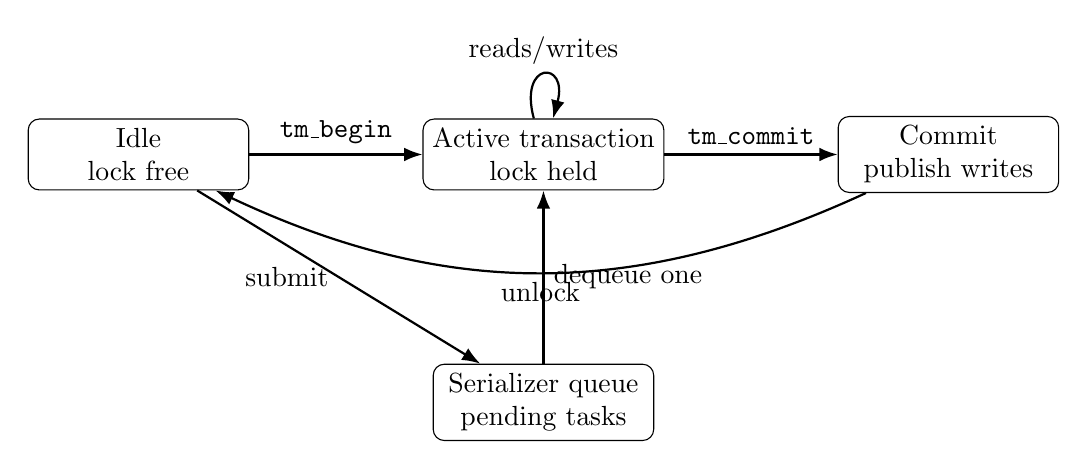
\begin{tikzpicture}[
    node distance=2.2cm,
    state/.style={draw, rounded corners, minimum width=2.8cm, minimum height=0.9cm, align=center},
    edge/.style={-{Latex}, thick}
]
\node[state] (idle) {Idle\\lock free};
\node[state, right=of idle] (active) {Active transaction\\lock held};
\node[state, right=of active] (commit) {Commit\\publish writes};
\node[state, below=of active] (queue) {Serializer queue\\pending tasks};

\draw[edge] (idle) -- node[above]{\texttt{tm\_begin}} (active);
\draw[edge] (active) -- node[above]{\texttt{tm\_commit}} (commit);
\draw[edge] (commit) to[bend left=25] node[below]{unlock} (idle);
\draw[edge] (queue) -- node[right]{dequeue one} (active);
\draw[edge] (idle) -- node[left]{submit} (queue);
\draw[edge] (active) to[loop above] node{reads/writes} (active);
\end{tikzpicture}
\caption{Non-speculative transactional execution. SGL admits one caller by a lock; a serializer admits one submitted task by a queue. Both execute at most one transaction body at a time.}
\label{fig:nonspec-state-machine}
\end{figure}

\begin{table}[htbp]
\centering
\begin{tabular}{p{0.22\linewidth}p{0.23\linewidth}p{0.23\linewidth}p{0.22\linewidth}}
\hline
Design & Serialization point & Main cost & Correctness argument \\
\hline
SGL & Global mutex at \texttt{tm\_begin} & Lock contention and lost parallelism & Mutual exclusion gives a single total order \\
Thread serializer & Worker dequeues one task & Submission, queueing, loss of locality & Worker order is the serialization order \\
DistributedSGL & Distributed lock or sequencer & Network latency and failure handling & One distributed owner at a time \\
PersistentSGL & Persistent critical section protocol & Flushes, fences, recovery metadata & Durable order follows lock-protected commit order \\
\hline
\end{tabular}
\caption{A taxonomy of non-speculative serializers. The mechanism changes, but the proof shape is the same: reduce execution to a sequential history.}
\label{tab:nonspec-taxonomy}
\end{table}

Amdahl's law gives the first-order bound. If fraction \(f\) of execution is serialized and \(N\) workers are available, the idealized speedup is

$$
S_{\max} = \frac{1}{f + \frac{1-f}{N}}
$$

where \(f\) is the non-parallel fraction and \(N\) is the number of cores. For SGL, transaction execution itself belongs to the serialized fraction. The exact value depends on the workload, but the shape is invariant: once all useful work is inside the global lock, more cores mostly add waiting.

\section{Thread‑Serializer / Queue‑Based TM}
\begin{itemize}
    \item A single worker thread executes transactions sequentially from a lock‑free queue.
    \item How this design eliminates contention on the lock but introduces submission overhead.
    \item Loss of thread-locality: transaction descriptors must be per-task, since work migrates across threads.
    \item The moral for later chapters: SGL is the baseline; every speculative design's job is to beat it without losing its guarantees.
\end{itemize}

A serializer is not merely an optimization of SGL. It changes the calling convention. The submitting thread no longer runs the transaction body; the worker does. Therefore transaction-local state cannot be stored only in thread-local variables of the submitter. The descriptor must travel with the task or be rebuilt by the worker.

\section{Worked Example: Bank Transfer Under SGL}
\label{sec:worked-sgl-bank}

The running bank example has two invariants. First, no account may fall below its floor. Second, the total amount of money is conserved by transfers. SGL enforces both by making each transfer execute as one sequential critical section.

\begin{lstlisting}[language=C++, caption={A compilable SGL-style transactional bank transfer.}]
#include <cassert>
#include <cstdint>
#include <iostream>
#include <mutex>
#include <numeric>
#include <stdexcept>
#include <thread>
#include <vector>

struct Account {
    std::int64_t balance;
    std::int64_t floor;
};

class SGLTM {
public:
    class Tx {
    public:
        explicit Tx(SGLTM& tm) : tm_(tm), active_(true) {
            tm_.lock_.lock();
        }

        Tx(const Tx&) = delete;
        Tx& operator=(const Tx&) = delete;

        ~Tx() {
            if (active_) {
                tm_.lock_.unlock();
            }
        }

        template <class T>
        T read(const T& x) const {
            return x;
        }

        template <class T>
        void write(T& x, const T& v) {
            x = v;
        }

        void commit() {
            if (!active_) {
                throw std::logic_error("double commit");
            }
            active_ = false;
            tm_.lock_.unlock();
        }

    private:
        SGLTM& tm_;
        bool active_;
    };

    Tx begin() {
        return Tx(*this);
    }

private:
    std::mutex lock_;
};

class Bank {
public:
    Bank(std::size_t n, std::int64_t initial, std::int64_t floor)
        : accounts_(n, Account{initial, floor}) {}

    bool transfer(std::size_t from, std::size_t to, std::int64_t amount) {
        if (from == to || from >= accounts_.size() || to >= accounts_.size()) {
            return false;
        }

        auto tx = tm_.begin();

        const std::int64_t from_balance = tx.read(accounts_[from].balance);
        const std::int64_t from_floor = tx.read(accounts_[from].floor);
        const std::int64_t to_balance = tx.read(accounts_[to].balance);

        if (from_balance - amount < from_floor) {
            tx.commit();
            return false;
        }

        tx.write(accounts_[from].balance, from_balance - amount);
        tx.write(accounts_[to].balance, to_balance + amount);

        tx.commit();
        return true;
    }

    std::int64_t total() const {
        return std::accumulate(
            accounts_.begin(), accounts_.end(), std::int64_t{0},
            [](std::int64_t s, const Account& a) { return s + a.balance; });
    }

private:
    SGLTM tm_;
    std::vector<Account> accounts_;
};

int main() {
    constexpr std::size_t accounts = 8;
    constexpr std::int64_t initial = 100;
    constexpr std::int64_t floor = 0;

    Bank bank(accounts, initial, floor);
    const std::int64_t before = bank.total();

    std::vector<std::thread> threads;
    for (std::size_t t = 0; t < 4; ++t) {
        threads.emplace_back([&bank, t] {
            for (int i = 0; i < 10000; ++i) {
                const std::size_t from = (t + i) % 8;
                const std::size_t to = (from + 1) % 8;
                bank.transfer(from, to, 1);
            }
        });
    }

    for (auto& th : threads) {
        th.join();
    }

    const std::int64_t after = bank.total();
    assert(before == after);
    std::cout << "money conserved: " << after << "\n";
}
\end{lstlisting}

Lessons:
\begin{itemize}
    \item The linearization point is the interval protected by the global mutex.
    \item Reads and writes still go through \texttt{read} and \texttt{write}. Replacing them with stubs during initialization can hide validation bugs in later backends.
    \item Failed transfers still commit a read-only transaction. There is no rollback path because no speculative write has escaped.
    \item The proof is independent of the number of calling threads: all completed transfers form the mutex acquisition order.
\end{itemize}

\section{Worked Example: Queue Serializer With Per-Task Descriptors}
\label{sec:worked-serializer-bank}

A serializer moves execution to a worker thread. The transaction descriptor is therefore attached to the submitted task. In this minimal example the descriptor is just the closure itself plus the returned future; real systems attach allocation logs, statistics, or backend-specific metadata.

\begin{lstlisting}[language=C++, caption={A compilable queue-based serializer for bank transfers.}]
#include <cassert>
#include <condition_variable>
#include <cstdint>
#include <future>
#include <iostream>
#include <mutex>
#include <numeric>
#include <queue>
#include <stdexcept>
#include <thread>
#include <type_traits>
#include <vector>
#include <functional>

struct Account {
    std::int64_t balance;
    std::int64_t floor;
};

class Serializer {
public:
    Serializer() : stopping_(false), worker_([this] { run(); }) {}

    Serializer(const Serializer&) = delete;
    Serializer& operator=(const Serializer&) = delete;

    ~Serializer() {
        {
            std::lock_guard<std::mutex> g(m_);
            stopping_ = true;
        }
        cv_.notify_one();
        worker_.join();
    }

    template <class F>
    auto submit(F&& f) -> std::future<std::invoke_result_t<F&>> {
        using R = std::invoke_result_t<F&>;

        auto task = std::make_shared<std::packaged_task<R()>>(
            std::forward<F>(f));
        std::future<R> result = task->get_future();

        {
            std::lock_guard<std::mutex> g(m_);
            if (stopping_) {
                throw std::runtime_error("submit after stop");
            }
            q_.push([task] { (*task)(); });
        }

        cv_.notify_one();
        return result;
    }

private:
    void run() {
        for (;;) {
            std::function<void()> job;

            {
                std::unique_lock<std::mutex> lk(m_);
                cv_.wait(lk, [this] { return stopping_ || !q_.empty(); });

                if (stopping_ && q_.empty()) {
                    return;
                }

                job = std::move(q_.front());
                q_.pop();
            }

            job();
        }
    }

    std::mutex m_;
    std::condition_variable cv_;
    std::queue<std::function<void()>> q_;
    bool stopping_;
    std::thread worker_;
};

class Bank {
public:
    Bank(std::size_t n, std::int64_t initial, std::int64_t floor)
        : accounts_(n, Account{initial, floor}) {}

    bool transfer_serial(std::size_t from, std::size_t to,
                         std::int64_t amount) {
        if (from == to || from >= accounts_.size() || to >= accounts_.size()) {
            return false;
        }

        Account& a = accounts_[from];
        Account& b = accounts_[to];

        if (a.balance - amount < a.floor) {
            return false;
        }

        a.balance -= amount;
        b.balance += amount;
        return true;
    }

    std::int64_t total_serial() const {
        return std::accumulate(
            accounts_.begin(), accounts_.end(), std::int64_t{0},
            [](std::int64_t s, const Account& a) { return s + a.balance; });
    }

private:
    std::vector<Account> accounts_;
};

int main() {
    Serializer ser;
    Bank bank(8, 100, 0);

    const std::int64_t before =
        ser.submit([&bank] { return bank.total_serial(); }).get();

    std::vector<std::future<bool>> replies;
    for (int i = 0; i < 40000; ++i) {
        replies.push_back(ser.submit([&bank, i] {
            const std::size_t from = static_cast<std::size_t>(i % 8);
            const std::size_t to = (from + 1) % 8;
            return bank.transfer_serial(from, to, 1);
        }));
    }

    for (auto& f : replies) {
        (void)f.get();
    }

    const std::int64_t after =
        ser.submit([&bank] { return bank.total_serial(); }).get();

    assert(before == after);
    std::cout << "money conserved: " << after << "\n";
}
\end{lstlisting}

Lessons:
\begin{itemize}
    \item The queue order is the serialization order.
    \item The bank object is unsynchronized internally; safety comes from the single worker.
    \item The submitter waits on a \texttt{future}. This makes latency visible even when the worker has no lock contention.
    \item Thread-local transaction descriptors would be wrong here: the submitting thread and executing thread are different.
\end{itemize}

\section{Summary}
\begin{itemize}
    \item Non‑speculative designs are correct by construction and serve as a baseline.
    \item Their lack of concurrency limits scalability.
    \item SGL is the simplest opacity proof in the book: every transaction observes a state produced by the previous committed transaction.
    \item Queue serializers replace lock handoff with task handoff. This can reduce lock contention but cannot create intra-transaction parallelism.
    \item In the companion codebase, SGL-like designs are not toys: they serve as reference backends and regression oracles alongside speculative systems such as NOrec, TL2, TSC-TM, SwissTM, and others. The reported test suites pass \texttt{test\_tx} 114/114 and \texttt{test\_ds} 207/207 for the implemented backends.
\end{itemize}

\section{Exercises}
\begin{enumerate}
    \item Calculate the maximum speedup achievable with a single‑global‑lock TM on a 16‑core machine when transactions spend 10\% of their time in a critical section.
    \item A serializing TM uses a single worker thread. Explain why this design can still outperform fine‑grained locking if transactions are very short and lock overhead dominates.
    \item Propose a hybrid design that starts with a non‑speculative execution and switches to speculative when contention is low. What information does the runtime need to make the switch?
    \item \emph{[implementation]} Extend Listing~\ref{sec:worked-sgl-bank} with \texttt{tm\_malloc} and \texttt{tm\_free} hooks. The hooks may still use the process allocator, but calls must pass through the backend object. Explain which tests would fail to detect bugs if initialization bypassed these hooks.
    \item \emph{[verification]} Write a PlusCal model of the bank transfer under SGL with two accounts, one lock, and two clients. State the money conservation invariant and the account-floor invariant. Model-check both with all transfer amounts in the set \texttt{\{0,1,2\}}.
    \item \emph{[theory]} Compare SGL and a queue serializer with three costs: lock acquisition, queue submission, and transaction body execution. Derive the condition under which the serializer has lower latency for a single transaction, and then explain why that condition may not imply higher throughput under a burst of requests.
\end{enumerate}


% -------------------------------------------------------------------
\chapter{Speculative Designs: NOrec and Beyond}
\section{NOrec: Value‑Based Validation}
\begin{itemize}
    \item Read‑set tracking via timestamps, write‑set buffering.
    \item Validation on every read and at commit time.
    \item PlusCal model and key invariants.
    \item Why `no ownership records': NOrec's write-set holds raw values, validated against a global sequence clock instead of per-location locks.
    \item The read-validate discipline: capture the clock, read the value, re-check the clock --- the same capture$\rightarrow$read$\rightarrow$recheck pattern that prevents partially-visible writes (Part~VII hardware echo).
    \item The invisible-it-committed trap: without value re-reading in validation, a concurrent commit between last read and commit sneaks a stale snapshot through (a real bug class fixed in the companion repo).
    \item Comparison layout: NOrec has the smallest metadata footprint of the in-memory STMs; validation cost grows with read-set size.
    \item Bloom-filter variant (NOrec-BF): a write-set bloom filter lets most reads skip read-set admission entirely --- read-mostly speedup at the cost of rare false positives.
\end{itemize}

\section{Worked Example: The NOrec Read Path}
\index{NOrec}\index{read-validate}\index{read-only transaction}\index{commit order}\index{validation}\index{read-set}
\label{sec:norec-example}

The read-validate discipline in code, mirroring \S\ref{sec:tso-example}'s
capture$\rightarrow$read$\rightarrow$recheck:

\begin{lstlisting}[language=C, caption={NOrec read: capture clock, read, re-check clock.}]
int32_t tm_read_i4(const void *addr) {
    for (;;) {
        uint64_t t1 = atomic_load(&g_clock);       /* capture   */
        int32_t v  = *(const int32_t*)addr;        /* read      */
        uint64_t t2 = atomic_load(&g_clock);       /* re-check  */
        if (t1 == t2) return v;                    /* consistent */
        /* a commit raced us: retry */
    }
}
\end{lstlisting}

\begin{itemize}
    \item Two clock reads bracket the data read; any interleaved commit changes the clock and forces a retry.
    \item This is the read-validate pattern the bullet above names --- the same one Part~II's store-buffer example revealed in hardware.
    \item Note there is no lock and no CAS: the read path is a plain load plus two acquires. That is the entire NOrec point.
    \item Exercise~1 of this chapter invites you to drop the second clock read and watch the invariant tests of Part~III fail.
\end{itemize}

\section{Worked Example: NOrec Bank Transfer}
\index{NOrec}\index{bank transfer}\index{money conservation}\index{account floor}\index{value-based validation}
\label{sec:norec-bank-transfer-example}

The running bank example is deliberately small: transfer money between two
accounts, preserve total money, and reject transfers that would take the
source account below its floor.  In NOrec, transaction-local writes are buffered
until commit; reads first consult the write-set, then perform the
capture$\rightarrow$read$\rightarrow$recheck protocol.

\begin{lstlisting}[language=C, caption={A compilable C++17 NOrec-style bank transfer with value revalidation.}]
#include <atomic>
#include <cstdint>
#include <mutex>
#include <unordered_map>
#include <vector>

struct ReadEntry {
    const int64_t *addr;
    int64_t value;
};

struct WriteEntry {
    int64_t *addr;
    int64_t value;
};

struct Tx {
    uint64_t start_clock = 0;
    std::vector<ReadEntry> read_set;
    std::vector<WriteEntry> write_set;
};

static std::atomic<uint64_t> g_clock{0};
static std::mutex g_commit_lock;

static bool validate(const Tx &tx) {
    for (const ReadEntry &r : tx.read_set) {
        if (*r.addr != r.value) return false;
    }
    return true;
}

static bool find_write(const Tx &tx, const int64_t *addr, int64_t &out) {
    for (auto it = tx.write_set.rbegin(); it != tx.write_set.rend(); ++it) {
        if (it->addr == addr) {
            out = it->value;
            return true;
        }
    }
    return false;
}

static int64_t tx_read(Tx &tx, int64_t *addr) {
    int64_t buffered = 0;
    if (find_write(tx, addr, buffered)) return buffered;

    for (;;) {
        uint64_t c1 = g_clock.load(std::memory_order_acquire);
        int64_t v = *addr;
        uint64_t c2 = g_clock.load(std::memory_order_acquire);

        if (c1 == c2 && validate(tx)) {
            tx.read_set.push_back(ReadEntry{addr, v});
            return v;
        }

        tx.read_set.clear();
        tx.start_clock = g_clock.load(std::memory_order_acquire);
    }
}

static void tx_write(Tx &tx, int64_t *addr, int64_t value) {
    for (WriteEntry &w : tx.write_set) {
        if (w.addr == addr) {
            w.value = value;
            return;
        }
    }
    tx.write_set.push_back(WriteEntry{addr, value});
}

static bool tx_commit(Tx &tx) {
    std::lock_guard<std::mutex> guard(g_commit_lock);

    if (!validate(tx)) return false;

    for (const WriteEntry &w : tx.write_set) {
        *w.addr = w.value;
    }

    g_clock.fetch_add(1, std::memory_order_release);
    return true;
}

static bool transfer(int64_t accounts[2],
                     int64_t floor[2],
                     int from,
                     int to,
                     int64_t amount) {
    Tx tx;
    tx.start_clock = g_clock.load(std::memory_order_acquire);

    int64_t src = tx_read(tx, &accounts[from]);
    int64_t dst = tx_read(tx, &accounts[to]);

    if (src - amount < floor[from]) return false;

    tx_write(tx, &accounts[from], src - amount);
    tx_write(tx, &accounts[to], dst + amount);

    return tx_commit(tx);
}

int main() {
    int64_t accounts[2] = {100, 100};
    int64_t floor[2] = {0, 0};

    bool ok = transfer(accounts, floor, 0, 1, 25);

    if (!ok) return 1;
    if (accounts[0] + accounts[1] != 200) return 2;
    if (accounts[0] < floor[0] || accounts[1] < floor[1]) return 3;

    return 0;
}
\end{lstlisting}

\begin{itemize}
    \item The money-conservation invariant is checked after commit: the sum of
    committed account balances remains unchanged.
    \item The floor check is speculative.  It is safe only because commit
    revalidates the values that justified it.
    \item The read path validates the old read-set before admitting a new read.
    Otherwise a transaction can assemble a snapshot from different commit
    times.
    \item NOrec has no per-account ownership record; the commit lock and global
    sequence clock serialize publication.
\end{itemize}

\begin{figure}[htbp]
\centering
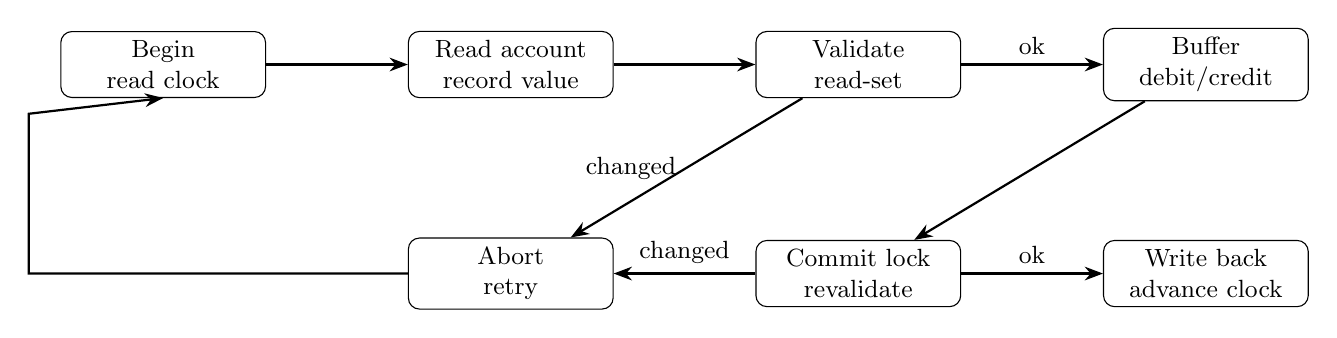
\begin{tikzpicture}[
    font=\small,
    node distance=1.8cm,
    box/.style={draw, rectangle, rounded corners, minimum width=2.6cm, minimum height=0.8cm, align=center},
    edge/.style={-{Stealth}, thick}
]
\node[box] (begin) {Begin\\read clock};
\node[box, right=of begin] (read) {Read account\\record value};
\node[box, right=of read] (validate) {Validate\\read-set};
\node[box, right=of validate] (buffer) {Buffer\\debit/credit};
\node[box, below=of validate] (commit) {Commit lock\\revalidate};
\node[box, left=of commit] (abort) {Abort\\retry};
\node[box, right=of commit] (publish) {Write back\\advance clock};

\draw[edge] (begin) -- (read);
\draw[edge] (read) -- (validate);
\draw[edge] (validate) -- node[above] {ok} (buffer);
\draw[edge] (buffer) -- (commit);
\draw[edge] (commit) -- node[above] {ok} (publish);
\draw[edge] (validate) -- node[left] {changed} (abort);
\draw[edge] (commit) -- node[above] {changed} (abort);
\draw[edge] (abort.west) -| ($(begin.south west)+(-0.4,-0.2)$) -- (begin.south);
\end{tikzpicture}
\caption{NOrec bank-transfer state machine.  The transaction may validate during reads and must validate again while holding the commit lock; only then may it publish both account updates and advance the global clock.}
\label{fig:norec-bank-state-machine}
\end{figure}


\section{TL2: The Textbook Global-Clock STM}
\begin{itemize}
    \item Global version clock read at begin; snapshot = transaction's start time.
    \item Write-set of (address, value) with per-location version metadata; read-set of (address, observed-value).
    \item Commit: acquire commit lock, re-validate read-set against the clock, write back under lock, advance clock, release.
    \item Timeline visualization (figure): two concurrent TL2 transactions and the clock values they observe.

\begin{figure}[ht]
\centering
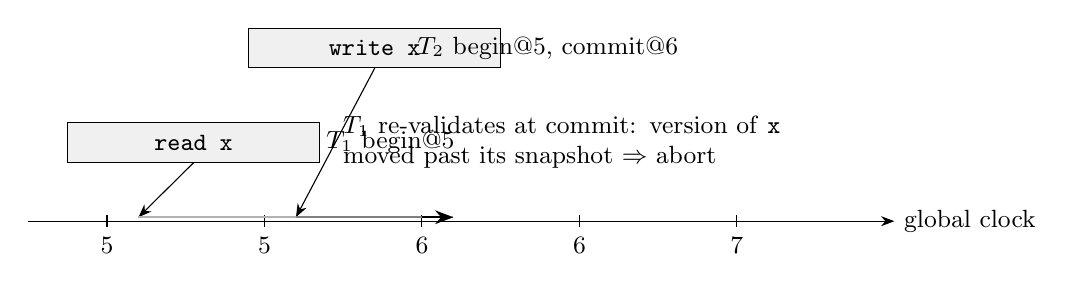
\begin{tikzpicture}[font=\small]
  % global clock timeline
  \draw[-{Stealth}] (0,0) -- (11,0) node[right] {global clock};
  \foreach \x/\lab in {1/$5$,3/$5$,5/$6$,7/$6$,9/$7$}
    \draw (\x,0.08) -- (\x,-0.08) node[below] {\lab};
  % T1: begins at 5, reads, then aborts after clock advances
  \node[draw,rectangle,minimum height=0.5cm,minimum width=3.2cm,fill=black!6]
        (T1) at (2.1,1.0) {\texttt{read x}};
  \draw[-{Stealth}] (T1.south) -- (1.4,0.05);
  \draw[-,thick,black!30] (1.4,0.05) -- (5.4,0.05);
  \node at (4.6,1.0) {$T_1$ begin@5};
  % T2: begins at 5, writes x, commits at clock 6
  \node[draw,rectangle,minimum height=0.5cm,minimum width=3.2cm,fill=black!6]
        (T2) at (4.4,2.2) {\texttt{write x}};
  \draw[-{Stealth}] (T2.south) -- (3.4,0.05);
  \draw[-,thick,black!50] (3.4,0.05) -- (5.0,0.05);
  \draw[-{Stealth},thick] (5.0,0.05) -- (5.4,0.05);
  \node at (6.6,2.2) {$T_2$ begin@5, commit@6};
  \node[align=left,text width=7.2cm] at (7.6,1.0)
        {$T_1$ re-validates at commit: version of \texttt{x}\\
         moved past its snapshot $\Rightarrow$ abort};
\end{tikzpicture}
\caption{TL2 timeline: $T_1$ and $T_2$ both begin at clock 5; $T_2$ commits (advancing the clock to 6) before $T_1$ validates, so $T_1$ must abort.}
\label{fig:tl2-timeline}
\end{figure}

    \item Validation semantics: every read-set entry must still match its recorded version, proving no writer committed during the transaction --- this is what makes invisible reads safe.
    \item Why TL2 is the standard baseline: minimal algorithm, clear invariants, easy to model-check (PlusCal model in the companion repo).
    \item The stored-value trap: without value-based re-validation, clock-only validation misfires on OCC write-back races --- the read-validate pattern recurs (see ROMULUS/MVLog case studies).
\end{itemize}

\section{TinySTM Design Variants}
\begin{itemize}
    \item Write‑through vs. write‑back (lazy version management).
    \item Eager locking vs. commit‑time locking.
    \item Comparison of strategies under different workloads.
    \item WBCTL (write-back, commit-time locking) vs.\ WT (write-through): the observable difference is \emph{where} the data lives before commit.
    \item Rollback mechanics: undo log for write-through, discard of write-set for write-back.
    \item Optimizations for the cache: versioned write-set entries, `read-set bypass' when a value matches the write-set, and when each pays off.
\end{itemize}

\section{Multiversion STMs: JVSTM and MVLog}
\begin{itemize}
    \item JVSTM: versioned boxes (VBox) store a history of (version, value) pairs; readers walk the newest body with version $\le$ read-version.
    \item Read-only transactions never abort: a consistent snapshot is read from history rather than validated.
    \item Commit: global clock increments under a lock; writer appends a new VBox body; validation compares VBox heads.
    \item MVLog: commit-slot negotiated at begin (a single \texttt{fetch\_add}), an ever-growing commit log of write-sets, and per-address newest-writer tracking.
    \item MVLog's `no-false-negative' bloom filter lets reads skip the log when the address is provably clean.
    \item The cost of history: memory grows with transaction count; reclamation (epochs, hazardous pointers) becomes a first-order concern.
    \item Why multiversion dominates GPU TM: read-only transactions never abort, and commit slots are cheap atomics (Part~VII, CSMV and GUST).
\end{itemize}

\section{Comparing the Family}
\index{comparison}\index{version management}\index{conflict detection}
\begin{itemize}
    \item A single table mapping design axes --- conflict detection (eager vs.\ lazy), version management (write-through vs.\ write-back), metadata (per-location locks vs.\ global clock), read set (invisible vs.\ validation-driven).
    \item NOrec bread-and-butter simplicity; TL2 clock-heavy but robust; TinySTM tuning knobs; multiversion for read-heavy and GPU workloads.
    \item The recurring invariant: every design must prevent a snapshot from becoming inconsistent mid-flight; the read-validate pattern is how software enforces it.
\end{itemize}

\begin{table}[ht]
\centering
\small
\begin{tabular}{lp{3.1cm}p{3.4cm}p{3.4cm}}
\hline
\textbf{Design} & \textbf{Read-set validation} & \textbf{Write-set ownership} & \textbf{Commit linearization} \\
\hline
SGL & none (mutex)           & direct writes under lock      & lock release \\
NOrec & clock-capture re-read & buffered, no locks            & clock advance \\
TL2 & per-location version   & buffered, commit lock         & clock advance + write-back \\
TinySTM WBCTL & lock/version check & commit-time locking           & lock release \\
TinySTM WT & versioned metadata   & write-through + undo log       & lock release \\
JVSTM & none (history walk)   & VBox append under lock        & clock increment \\
MVLog & no-false-negative bloom & commit-log slot + index      & slot publish \\
\hline
\end{tabular}
\caption{The comparison matrix used throughout this chapter and the exercises: each row gives the same four facts --- read validation rule, write ownership, and the linearization point. A backend ``family'' is a choice in each column; opacity arguments in Part~III are written column-by-column.}
\label{tab:family-matrix}
\end{table}

\begin{itemize}
    \item \textbf{Per-runtime performance signatures} (the expected bottleneck of each row in Table~\ref{tab:family-matrix}): SGL serializes everything (throughput cap $=1/\text{tx time}$); NOrec validates whole read-sets (cost grows with read-set size); TL2 pays commit-lock serialization plus clock reads; TinySTM pays per-location metadata traffic; multiversion pays memory reclamation.
    \item Exercise~6 turns Table~\ref{tab:family-matrix} into numbers: the memory-overhead row is measurable on the repository's benchmarks.
\end{itemize}

\section{Backend Taxonomy: The Repository in One Table}
\index{backend taxonomy}\index{SGL}\index{TinySTM}\index{WBCTL}\index{NOrec}\index{TL2}\index{MVLog}\index{JVSTM}\index{SwissTM}\index{Romulus}\index{XTM}\index{TSX}\index{GPU TM}\index{persistent TM}\index{distributed TM}\index{reclamation}\index{private memory}\index{memory reclamation}
The companion repository contains 20+ runtimes. This book explains the
families; the table maps \emph{which repository backend is which family},
so a reader looking for ``where is the code for X'' can find it and so the
prose never overclaims that every backend is analysed in depth:

\begin{table}[ht]
\centering
\small
\begin{tabular}{lll}
\hline
\textbf{Repository backend} & \textbf{Family} & \textbf{Chapter} \\
\hline
\texttt{sgl}                 & single global lock   & Ch.~8 \\
\texttt{tsxsgl}, \texttt{spht} & HTM + SGL fallback  & Ch.~8, 16 \\
\texttt{norec}, \texttt{norec\_bf} & value-based validation & Ch.~9 \\
\texttt{tl2}, \texttt{tsc\_tm}     & global-clock OCC     & Ch.~9 \\
\texttt{tinystm} (\texttt{wbctl}/\texttt{wt}/\texttt{wbetl}) & per-object locking & Ch.~9 \\
\texttt{jvstm}, \texttt{mvlog}      & multiversion         & Ch.~9 \\
\texttt{swisstm}, \texttt{romulus}, \texttt{leftright} & OCC variants & Ch.~9 \\
\texttt{xtm}, \texttt{dudetm}, \texttt{nvhtm} & page/persistent/hybrid & Ch.~13 \\
\texttt{persistent\_sgl}, \texttt{distributed\_sgl}, \texttt{tikv} & persistent/distributed & Ch.~18 \\
\texttt{gust}, \texttt{csmv}, \texttt{jvstm-gpu}, \texttt{gputx}, \texttt{gacco}, \texttt{gpu\_stm} & GPU warp TM & Ch.~17 \\
\hline
\end{tabular}
\caption{Repository backend $\rightarrow$ family $\rightarrow$ where it is discussed. Backends without a dedicated prose section are still exercised by the benchmark suite and, where present, have a PlusCal/TLA+ model (Table~\ref{tab:traceability}).}
\label{tab:backend-taxonomy}
\end{table}

\section{Semantic Obligations Checklist}
\label{sec:semantic-obligations}
Part~I introduced opacity, sandboxing, and privatization; here is where
each is \emph{discharged} by a concrete runtime mechanism, so no promise
from Chapter~2 floats unresolved:

\begin{itemize}
    \item \textbf{Opacity} $\rightarrow$ Ch.~9 read-validate discipline (\S\ref{sec:norec-example}) and the TLA+ invariants of Table~\ref{tab:traceability}.
    \item \textbf{Sandboxing} $\rightarrow$ Ch.~13 memory management: speculative writes must live in the write-set or the TM region, never the caller's heap.
    \item \textbf{Privatization} $\rightarrow$ Ch.~9 (publishing objects) and Ch.~13: a committed object handed to a non-transactional thread must be fully written back before publication.
    \item \textbf{Irrevocability} (operations that cannot abort, e.g.\ I/O) $\rightarrow$ Ch.~8's serializing designs and Ch.~13's policy.
    \item \textbf{Memory reclamation} (when may a freed address be reused) $\rightarrow$ Ch.~13: deferred frees and the double-free hazards of region allocators.
    \item \textbf{Signal safety} (what \texttt{siglongjmp} may do inside a transaction) $\rightarrow$ Ch.~13's policy section.
    \item \textbf{Compiler obligations} (which accesses must stay instrumented) $\rightarrow$ the contract of Chapter~11.
\end{itemize}

\section{Worked Example: The TL2 Commit Path}
\index{TL2}\index{commit protocol}\index{commit lock}\index{global clock}\index{OCC}\index{validation}\index{version management}
\label{sec:tl2-example}

The five-phase commit that Chapter~6's model and Part~III's invariants check:

\begin{lstlisting}[language=C, caption={TL2 commit: lock, validate, write back, publish.}]
bool tm_end(void) {
    if (!commit_lock.try_lock()) return retry();        /* 1. serialise */
    for (each r in read_set)                            /* 2. validate */
        if (version_of(r.addr) != r.observed_version)
            { commit_lock.unlock(); return retry(); }
    uint64_t ts = global_clock.fetch_add(1) + 1;        /* 3. new version */
    for (each w in write_set) {                         /* 4. write back */
        *(w.addr) = w.value;
        store_version(w.addr, ts);
    }
    commit_lock.unlock();                               /* 5. publish   */
    return true;
}
\end{lstlisting}

\begin{itemize}
    \item Step 2 is the expensive one: the read-set is validated against per-location version metadata, not a global clock.
    \item Step 4 writes back \emph{under} the commit lock, then advances the clock so no concurrent reader can observe a half-published write-set.
    \item The stored-value trap is step 4 interacting with step 2: without the read-validate pattern of \S\ref{sec:norec-example}, a stale read-set can validate against an old version while the write-back overwrites a newer commit.
    \item The same five steps appear in the PlusCal model of Part~III, and in the GPU backends of Part~VII at warp granularity.
\end{itemize}

\section{Worked Example: Account-Floor PlusCal Model}
\index{PlusCal}\index{TLA+}\index{model checking}\index{account floor}\index{money conservation}
\label{sec:pluscal-bank-floor-example}

The model below is intentionally small enough for TLC.  Two processes repeatedly
try to transfer one unit in opposite directions.  The commit action is atomic:
it checks the floor against the current state and then updates both accounts.
This is the serial specification that NOrec, TL2, TinySTM, JVSTM, and MVLog
must refine.

\begin{lstlisting}[language={}, caption={PlusCal/TLA+ model of two-account transfer with conservation and floor invariants.}]
---- MODULE BankTransferFloor ----
EXTENDS Naturals, TLC

CONSTANT Init0, Init1, Floor0, Floor1

ASSUME Init0 >= Floor0 /\ Init1 >= Floor1

(*
--algorithm Bank
variables bal = [0 |-> Init0, 1 |-> Init1];

define
  TotalOK == bal[0] + bal[1] = Init0 + Init1
  FloorsOK == bal[0] >= Floor0 /\ bal[1] >= Floor1
end define;

process (P \in {0, 1})
variables from = P, to = 1 - P, amount = 1;
begin
Loop:
  while TRUE do
    if bal[from] - amount >=
       IF from = 0 THEN Floor0 ELSE Floor1 then
      bal[from] := bal[from] - amount;
      bal[to] := bal[to] + amount;
    end if;
  end while;
end process;
end algorithm;
*)

==== 
\end{lstlisting}

A minimal TLC configuration is:

\begin{lstlisting}[language={}, caption={TLC configuration for the PlusCal account-floor model.}]
SPECIFICATION Spec
CONSTANTS
  Init0 = 2
  Init1 = 2
  Floor0 = 0
  Floor1 = 0
INVARIANTS
  TotalOK
  FloorsOK
\end{lstlisting}

\begin{itemize}
    \item The invariant \texttt{TotalOK} is the money-conservation property:
    transfers move value; they do not create or destroy it.
    \item The invariant \texttt{FloorsOK} is the safety property enforced by
    the transactional read of the source account followed by validation.
    \item To model a broken STM, split the guarded update into separate read,
    validate, debit, and credit actions, then remove the final validation.
    TLC should find an execution where the guard was true for a stale source
    value.
    \item This model is a serial specification, not an implementation model.
    The implementation models add clocks, read-sets, write-sets, locks, or
    version histories.
\end{itemize}

\begin{table}[htbp]
\centering
\small
\begin{tabular}{llll}
\hline
\textbf{Backend family} & \textbf{Snapshot mechanism} & \textbf{Read-only aborts} & \textbf{Main cost} \\
\hline
NOrec & global clock + value re-read & possible & read-set validation \\
NOrec-BF & global clock + bloom-filter bypass & possible & false positives and validation \\
TL2/TSC-TM & start timestamp + per-location versions & possible & metadata traffic and commit lock \\
TinySTM WBCTL & per-location lock/version words & possible & ownership metadata \\
TinySTM WT & write-through + undo log & possible & rollback and eager conflicts \\
JVSTM & version history walk & no & history retention \\
MVLog & commit log + newest-writer index & no for stable snapshots & log scan and reclamation \\
\hline
\end{tabular}
\caption{Snapshot mechanisms in the speculative STM family.  The measured repository results match the expected signatures: TL2 and TSC-TM are close on the M1 Pro bank/fuzz workload, NOrec-BF improves read-mostly NOrec, and MVLog pays for history and log management.}
\label{tab:snapshot-taxonomy}
\end{table}


\section{Summary}
\begin{itemize}
    \item Speculation unlocks concurrency but introduces aborts.
    \item Different version‑management policies trade off simplicity for performance.
    \item The design space is small: clocks, locks, logs, and history --- every real STM is a combination of these.
\end{itemize}

\section{Exercises}
\begin{enumerate}
    \item In NOrec, T1 writes to \texttt{x}, then T2 writes to \texttt{x} and commits. Explain why T1 will abort.
    \item TinySTM can be configured for eager locking or commit‑time locking. Given a workload with high contention on a single location, predict which mode will perform better and justify your answer.
    \item Design a simple experiment using the STAMP benchmark suite to compare the abort rates of NOrec and TinySTM’s write‑through variant.
    \item In TL2, explain why the read-set validation must re-read the metadata (not just remember the snapshot) and sketch the read-validate pattern that prevents a partially committed write from being observed.
    \item Write a PlusCal model of a TL2 commit that omits the read-set re-validation, and run TLC to produce a counterexample (Part~III workflow).
    \item Compare memory overhead: NOrec, TL2, JVSTM, and MVLog, for a workload with a large read-set and small write-set.
    \item \emph{[implementation]} Modify the NOrec bank-transfer example in \S\ref{sec:norec-bank-transfer-example} to retry aborted transactions in a bounded loop.  Report separately the number of floor rejections and validation aborts.
    \item \emph{[verification]} Extend the PlusCal model in \S\ref{sec:pluscal-bank-floor-example} with a speculative local variable \texttt{seen}.  Split the transfer into read, check, debit, and credit actions, then add a commit-time validation action.  Show which invariant fails when the validation action is removed.
    \item \emph{[theory]} In Table~\ref{tab:snapshot-taxonomy}, identify which families implement invisible reads.  For each such family, state the proof obligation that prevents an inconsistent snapshot from being committed.
\end{enumerate}

% -------------------------------------------------------------------
%  PART V: COMPILER INSTRUMENTATION FOR TM
% -------------------------------------------------------------------
\part{Compiler Instrumentation for TM}

\chapter{Compiler Fundamentals – IRs and Passes}
\section{The Compilation Pipeline}
\begin{itemize}
    \item Front end (lexing, parsing, AST), middle end (IR optimization), back end (code generation).
    \item LLVM IR and GCC GIMPLE: a high‑level view.
\end{itemize}

\begin{figure}[htbp]
\centering
\resizebox{\textwidth}{!}{%
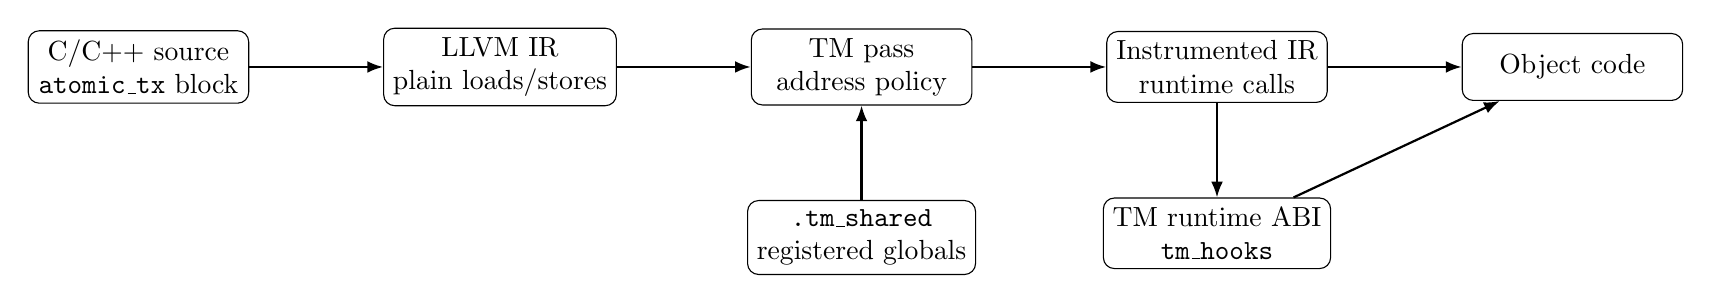
\begin{tikzpicture}[
    node distance=1.7cm,
    box/.style={draw, rounded corners, minimum width=2.8cm, minimum height=0.85cm, align=center},
    smallbox/.style={draw, rounded corners, minimum width=2.4cm, minimum height=0.75cm, align=center},
    arr/.style={-{Latex[length=2mm]}, thick}
]
\node[box] (src) {C/C++ source\\\texttt{atomic\_tx} block};
\node[box, right=of src] (ir) {LLVM IR\\plain loads/stores};
\node[box, right=of ir] (pass) {TM pass\\address policy};
\node[box, right=of pass] (iir) {Instrumented IR\\runtime calls};
\node[box, right=of iir] (obj) {Object code};

\node[smallbox, below=1.2cm of pass] (shared) {\texttt{.tm\_shared}\\registered globals};
\node[smallbox, below=1.2cm of iir] (abi) {TM runtime ABI\\\texttt{tm\_hooks}};

\draw[arr] (src) -- (ir);
\draw[arr] (ir) -- (pass);
\draw[arr] (pass) -- (iir);
\draw[arr] (iir) -- (obj);
\draw[arr] (shared) -- (pass);
\draw[arr] (iir) -- (abi);
\draw[arr] (abi) -- (obj);
\end{tikzpicture}%
}
\caption{A compiler TM pass sits between IR optimization and code generation; its output is ordinary code with calls into the runtime ABI.}
\label{fig:compiler-tm-pass}
\end{figure}

\section{Instrumentation as a Compiler Pass}
\begin{itemize}
    \item Replacing transactional memory accesses with calls to a runtime.
    \item The structure of a \texttt{FunctionPass} in LLVM (and its GIMPLE equivalent).
    \item Pseudocode for the instrumentation algorithm, plus a PlusCal specification.
    \item What a production pass must handle: function calls into uninstrumented code, indirect calls, and escaping pointers.
    \item The instrumentation decision is a static-address-space question: heap/global addresses go through TM; stack addresses bypass it (the \texttt{LLVM\_TM\_ADDR\_CHECK} pattern).
    \item Where TM globals get registered so the runtime can recognise them (the \texttt{.tm\_shared} section of the companion implementation).
    \item Trade-off: instrumenting every load/store (simple, slow) vs.\ annotating shared data (fast, needs programmer discipline).
\end{itemize}

\begin{table}[htbp]
\centering
\begin{tabular}{p{0.22\linewidth}p{0.28\linewidth}p{0.22\linewidth}p{0.16\linewidth}}
\hline
Policy & What the pass rewrites & Programmer\slash{}runtime obligation & Typical cost \\
\hline
Instrument every load/store & All memory operations inside a transaction become runtime calls. & Runtime must cheaply reject private addresses or tolerate over-instrumentation. & Highest; simple and conservative. \\
Static address-space check & Heap and global addresses are instrumented; provable stack addresses bypass TM. & Alias analysis must be conservative when provenance is unclear. & Lower; still safe when uncertain cases are instrumented. \\
Annotated shared section & Only data registered in \texttt{.tm\_shared} is treated as transactional shared state. & Programmer or front end must mark all shared transactional objects. & Lowest common overhead; weakest if annotations are wrong. \\
Manual runtime calls & Source code calls \texttt{tm\_read\_*} and \texttt{tm\_write\_*} directly. & Programmer maintains ABI discipline by hand. & Useful for tests and microbenchmarks; brittle at scale. \\
\hline
\end{tabular}
\caption{Instrumentation policies differ mainly in where the conservative decision is made: compiler, runtime, or programmer.}
\label{tab:instrumentation-policies}
\end{table}

\section{Worked Example: A Load, Before and After the Pass}
\index{instrumentation}\index{LLVM IR}
\label{sec:ir-example}

IR is the right place to see what instrumentation actually changes. A single
transactional read of an \texttt{int} becomes a call into the runtime:

\begin{lstlisting}[language=C, caption={LLVM IR for a transactional load, before and after instrumentation.}]
; before the pass -- a plain memory load
%1 = load i32, i32* %p

; after the pass -- the load is replaced by a runtime call
%1 = call i32 @__tm_read_i4(i32* %p)
\end{lstlisting}

\begin{itemize}
    \item The pass rewrites the memory operand of each load/store into a typed runtime call (\texttt{tm\_read\_i4}, \texttt{tm\_write\_i4}, \ldots).
    \item The static address-space policy decides \emph{which} accesses get rewritten: heap/global go through TM, stack addresses bypass via \texttt{LLVM\_TM\_ADDR\_CHECK}.
    \item The type in the call name matters: \texttt{i4} vs \texttt{i8} select different runtime fast paths and different read-set log widths.
    \item Exercise~1 of this chapter asks you to repeat this mapping by hand on a GIMPLE listing.
    \item The contract the pass instruments \emph{against} --- the exact signatures of \texttt{tm\_read\_*}\slash{}\texttt{tm\_write\_*}, how a transaction begins/ends, and what an abort unwinds --- is the runtime ABI of Chapter~7. If the ABI moves, the pass must move with it; the two are coupled by design, which is why they share the \texttt{tm\_hooks} table rather than a hard-coded call.
\end{itemize}

\section{Worked Example: Instrumenting a Bank Transfer}
\index{bank transfer}\index{runtime ABI}
\label{sec:bank-transfer-instrumented-c}

This listing is not an implementation of NOrec, TL2, or TSC-TM. It is the
shape of the code produced by the pass: ordinary source-level loads and stores
have become calls through the transactional ABI. The stub runtime below makes
the file compile and lets the invariant be tested in a single-threaded run.

\begin{lstlisting}[language=C, caption={Compilable C++17 model of an instrumented bank transfer.}]
#include <assert.h>
#include <stdint.h>

struct Account {
    int balance;
};

extern "C" void __tm_begin(void) {
    /* Real backends allocate per-transaction metadata here. */
}

extern "C" void __tm_end(void) {
    /* Real backends validate and commit here. */
}

extern "C" int __tm_read_i4(const int *p) {
    return *p;
}

extern "C" void __tm_write_i4(int *p, int value) {
    *p = value;
}

static int sum2(const Account *a, const Account *b) {
    return a->balance + b->balance;
}

/* This is the post-pass shape of:
 *
 *   atomic_tx {
 *       if (from->balance - amount >= floor) {
 *           from->balance -= amount;
 *           to->balance += amount;
 *       }
 *   }
 */
static void transfer_instrumented(Account *from,
                                  Account *to,
                                  int amount,
                                  int floor) {
    __tm_begin();

    int from_balance = __tm_read_i4(&from->balance);
    int to_balance   = __tm_read_i4(&to->balance);

    if (from_balance - amount >= floor) {
        __tm_write_i4(&from->balance, from_balance - amount);
        __tm_write_i4(&to->balance,   to_balance + amount);
    }

    __tm_end();
}

int main(void) {
    Account a = { 100 };
    Account b = {  40 };

    int before = sum2(&a, &b);
    transfer_instrumented(&a, &b, 30, 50);
    int after = sum2(&a, &b);

    assert(a.balance >= 50);
    assert(before == after);

    before = after;
    transfer_instrumented(&a, &b, 80, 50);
    after = sum2(&a, &b);

    assert(a.balance >= 50);
    assert(before == after);
    return 0;
}
\end{lstlisting}

Lessons:
\begin{itemize}
    \item The compiler pass does not prove the money-conservation invariant; it preserves the memory operations on which the runtime will enforce atomicity.
    \item The two writes must be in one transaction. Instrumenting each store independently would preserve type correctness but not the bank invariant under concurrency.
    \item The generated calls are typed. Here \texttt{balance} is an \texttt{int}, so the pass emits \texttt{\_\_tm\_read\_i4} and \texttt{\_\_tm\_write\_i4}.
    \item Stack temporaries such as \texttt{from\_balance}, \texttt{to\_balance}, and \texttt{before} are not shared transactional locations and should not be routed through the TM runtime.
\end{itemize}

\section{Worked Example: Model Checking the Address Policy}
\index{TLA+}\index{address-space check}
\label{sec:address-policy-tla}

The pass has a small but important safety rule: do not instrument provably
private stack locations; do instrument heap and global locations. The following
TLA+ module models one pass over a three-instruction program and checks that
the emitted operation stream respects that rule.

\begin{lstlisting}[caption={TLA+ model of the stack-bypass/shared-instrument policy.}]
---- MODULE InstrumentPass ----
EXTENDS TLC, Sequences, Naturals

VARIABLES pc, out

Ops == {"load", "store"}
Addrs == {"stack", "heap", "global"}
Kinds == {"plain", "tmread", "tmwrite"}

Prog ==
  << [op |-> "load",  addr |-> "stack"],
     [op |-> "store", addr |-> "heap"],
     [op |-> "load",  addr |-> "global"] >>

Instr(op, addr) ==
  IF addr = "stack" THEN
      "plain"
  ELSE IF op = "load" THEN
      "tmread"
  ELSE
      "tmwrite"

Init ==
  /\ pc = 1
  /\ out = << >>

Next ==
  IF pc <= Len(Prog) THEN
      /\ out' = Append(out, Instr(Prog[pc].op, Prog[pc].addr))
      /\ pc' = pc + 1
  ELSE
      /\ UNCHANGED << pc, out >>

TypeOK ==
  /\ pc \in 1..(Len(Prog) + 1)
  /\ out \in Seq(Kinds)
  /\ Len(out) <= Len(Prog)

StackBypass ==
  \A i \in 1..Len(out):
    Prog[i].addr = "stack" => out[i] = "plain"

SharedInstrumented ==
  \A i \in 1..Len(out):
    Prog[i].addr # "stack" =>
      ((Prog[i].op = "load"  => out[i] = "tmread") /\
       (Prog[i].op = "store" => out[i] = "tmwrite"))

Spec == Init /\ [][Next]_<< pc, out >>

====
\end{lstlisting}

Lessons:
\begin{itemize}
    \item The model is deliberately smaller than LLVM. It isolates the address-policy obligation from parsing, dominance, and code generation.
    \item \texttt{StackBypass} catches accidental over-instrumentation of private stack slots.
    \item \texttt{SharedInstrumented} catches the dangerous bug: a heap or global access escaping the TM runtime.
    \item In a production pass, the hard case is not the rule itself but proving that an address is stack-private after optimization and aliasing.
\end{itemize}

\section{Summary}
\begin{itemize}
    \item Instrumentation is a source‑to‑source (or IR‑to‑IR) transformation.
    \item A pass that instruments every memory access is the simplest possible TM compiler support.
    \item A production-quality pass needs an address-space policy, a shared-data registry, and careful handling of uninstrumented callees.
\end{itemize}

\section{Exercises}
\begin{enumerate}
    \item Given a small C function, manually identify which GIMPLE statements would be replaced by calls to a TM runtime barrier.
    \item Critique a naive instrumentation pass that instruments all loads and stores in the whole program. What performance problems would arise?
    \item Design an LLVM pass that instruments only loads and stores inside basic blocks marked with a special intrinsic.
\end{enumerate}

% -------------------------------------------------------------------
\chapter{Compiler Optimizations and Their Impact on TM}
\section{Common Optimizations}
\begin{itemize}
    \item Dead‑store elimination (DSE), loop‑invariant code motion (LICM), common subexpression elimination (CSE).
    \item Each can silently break transactional semantics by eliminating or reordering instrumented accesses.
    \item The root problem: most optimizers assume a single-threaded execution model and treat memory accesses as opaque only when told to.
    \item Optimizations inside a transaction must be rerun \emph{after} instrumentation, not before, or the pass rediscovers and undoes TM calls.
    \item Stack versus shared memory: it is safe to optimize stack accesses aggressively; shared/global accesses inside a transaction are the only dangerous ones.
\end{itemize}

\section{Worked Example: Two Optimizations That Break TM}
\index{DSE}\index{LICM}
\label{sec:optim-example}

Take the canonical transfer body, already instrumented. Two well-meaning
optimizations silently delete transactional effects:

\begin{lstlisting}[language=C, caption={DSE and LICM on an instrumented transaction.}]
/* DSE: the compiler sees a store with no later use in this function. */
int v = tm_read_i4(&a->balance);
tm_write_i4(&a->balance, v - n);      /* result never read here */
return 0;                             /* DSE discards the store! */

/* LICM: a transactional read is loop-invariant under LICM. */
for (int i = 0; i < 100; ++i)
    sum += tm_read_i4(&b[i]);         /* hoisted out of the loop,
                                         reads b[0] once */
\end{lstlisting}

\begin{itemize}
    \item Both are correct under single-threaded semantics and both are wrong for TM: the write must reach the write-set, and the read must see fresh data each iteration.
    \item The fix is the contract of the next section: \texttt{tm\_clobber} and the rule that instrumentation runs \emph{after} optimization.
    \item These are exactly the ``mismatch bugs seen in the wild'' of the next section --- pass reordering and dead-store elimination of speculative writes.
\end{itemize}

\section{The Instrumentation Contract}
\label{sec:instrumentation-contract}
The precise, mechanical rules a compiler pass and a TM runtime agree on.
This section turns the previous section's warnings into a checkable list.

\begin{itemize}
    \item \textbf{Which accesses are instrumented.} Heap and shared-global memory operands inside a transaction are rewritten to \texttt{tm\_read\_*}/\texttt{tm\_write\_*} calls; stack-locals bypass via \texttt{LLVM\_TM\_ADDR\_CHECK}. The \texttt{[[tm::shared]]} annotation (Chapter~4) is the source-level way to put a global on the instrumented side.
    \item \textbf{Which are exempt.} Accesses that provably target the current thread's stack, addresses registered in the runtime's TM-global registry, and operations in uninstrumented (e.g.\ \texttt{transaction\_pure}) callees are left untouched.
    \item \textbf{What metadata is preserved.} The pass must not lose the address-space classification or the width of each access --- the call name itself (\texttt{i4} vs.\ \texttt{i8}) encodes both, so type-preserving rewrites are mandatory.
    \item \textbf{Pass ordering.} Instrumentation is the \emph{last} memory-affecting pass: anything that eliminates or reorders memory operations must run before it. Running DSE or LICM after instrumentation silently discards read-set/write-set side effects (Section~\ref{sec:optim-example}).
    \item \textbf{Barriers for the optimizer.} Calls to \texttt{tm\_read\_*}/\texttt{tm\_write\_*} are opaque side-effecting calls --- they must be marked \texttt{tm\_clobber}-equivalent so the optimizer never treats them as pure loads/stores.
\end{itemize}

\section{Worked Example: Barriered Transfer Instrumentation}
\index{tm\_clobber}
\label{sec:worked-barriered-transfer}

The following small C file is intentionally boring. That is the point: the
compiler may optimize stack temporaries, but it must not delete or reorder the
transactional calls that construct the read-set and write-set.

\begin{lstlisting}[language=C, caption={A compilable transfer body with opaque TM accessors.}]
#include <stdint.h>
#include <stdio.h>
#include <stdlib.h>

typedef struct Account {
    int32_t balance;
} Account;

typedef struct Tx {
    int writes;
} Tx;

/* In a real backend these enter the read-set and write-set.  The attributes
   force the compiler to treat the calls as side-effecting boundaries. */
__attribute__((noinline))
static int32_t tm_read_i4(Tx *tx, const int32_t *p) {
    (void)tx;
    __asm__ __volatile__("" ::: "memory");
    return *p;
}

__attribute__((noinline))
static void tm_write_i4(Tx *tx, int32_t *p, int32_t v) {
    __asm__ __volatile__("" ::: "memory");
    *p = v;
    tx->writes++;
    __asm__ __volatile__("" ::: "memory");
}

static int transfer(Tx *tx, Account *from, Account *to,
                    int32_t amount, int32_t floor) {
    int32_t from0 = tm_read_i4(tx, &from->balance);
    int32_t to0   = tm_read_i4(tx, &to->balance);

    if (from0 - amount < floor)
        return 0;              /* abort or user-level failed transfer */

    /* These stores are live even if this function never reads them again. */
    tm_write_i4(tx, &from->balance, from0 - amount);
    tm_write_i4(tx, &to->balance,   to0 + amount);
    return 1;
}

int main(void) {
    Account a = { .balance = 100 };
    Account b = { .balance =  50 };
    Tx tx = { .writes = 0 };

    int ok = transfer(&tx, &a, &b, 30, 0);
    if (!ok || a.balance != 70 || b.balance != 80 || tx.writes != 2)
        return EXIT_FAILURE;

    puts("transfer committed");
    return EXIT_SUCCESS;
}
\end{lstlisting}

\begin{itemize}
    \item \texttt{from0}, \texttt{to0}, and \texttt{ok} are ordinary stack values; scalar replacement and register allocation are harmless there.
    \item \texttt{tm\_write\_i4} is not a dead store. It is the operation that records the speculative update.
    \item The inline memory clobber models the minimum compiler contract. Production runtimes encode the same idea with ABI attributes, intrinsics, or opaque calls.
    \item The bank invariant is not a local property of the function body. It is preserved only if both writes survive to commit.
\end{itemize}

\begin{figure}[htbp]
\centering
\resizebox{\textwidth}{!}{%
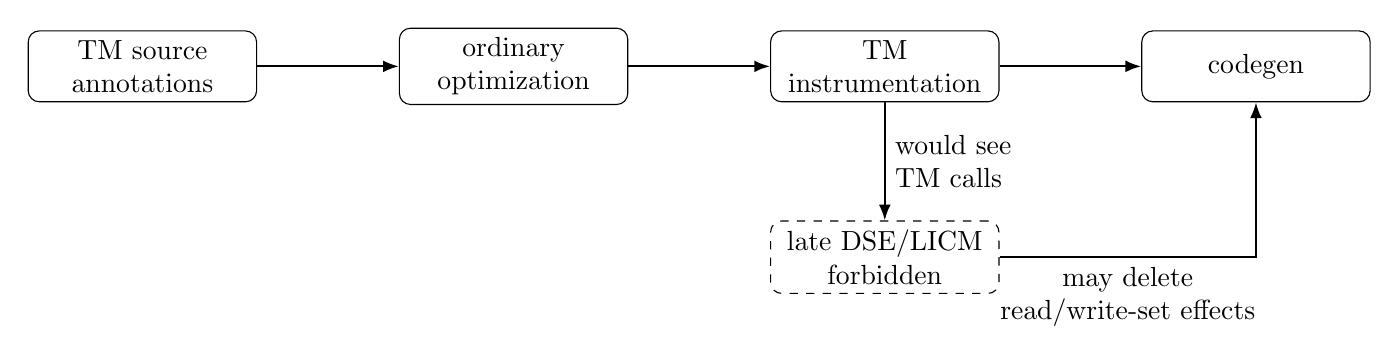
\begin{tikzpicture}[
    node distance=1.5cm and 1.8cm,
    box/.style={draw, rounded corners, align=center, minimum width=2.9cm, minimum height=0.9cm},
    bad/.style={draw, rounded corners, align=center, minimum width=2.9cm, minimum height=0.9cm, dashed},
    arr/.style={-{Latex[length=2mm]}, thick}
]
\node[box] (src) {TM source\\annotations};
\node[box, right=of src] (opt) {ordinary\\optimization};
\node[box, right=of opt] (inst) {TM\\instrumentation};
\node[box, right=of inst] (code) {codegen};

\node[bad, below=of inst] (late) {late DSE/LICM\\forbidden};

\draw[arr] (src) -- (opt);
\draw[arr] (opt) -- (inst);
\draw[arr] (inst) -- (code);
\draw[arr] (inst) -- node[right, align=left] {would see\\TM calls} (late);
\draw[arr] (late) -| node[pos=0.25, below, align=center] {may delete\\read/write-set effects} (code);
\end{tikzpicture}%
}
\caption{Safe pass ordering for TM compilation. Memory-changing optimizations run before instrumentation; afterward, transactional read and write calls are opaque side effects.}
\label{fig:tm-pass-ordering}
\end{figure}

\section{Optimization Taxonomy}
\index{compiler optimization}
\label{sec:optimization-taxonomy}

Table~\ref{tab:tm-optimization-taxonomy} separates optimizations by what they
may legally do in a TM-aware compiler. The useful rule is not ``turn the
optimizer off.'' It is ``keep ordinary optimizations on values that cannot be
shared; preserve transactional effects on values that can be shared.''

\begin{table}[htbp]
\centering
\begin{tabular}{p{0.18\linewidth} p{0.30\linewidth} p{0.38\linewidth}}
\hline
Optimization & Unsafe pattern inside a transaction & TM-aware rule \\
\hline
DSE & Removes \texttt{tm\_write\_*} because no later load observes it in the same function. & Treat write instrumentation as an opaque side effect. A speculative write is live until abort or commit. \\
LICM & Hoists \texttt{tm\_read\_*} out of a loop because the address expression is syntactically invariant. & Do not move transactional reads across iteration, validation, abort, or commit boundaries unless the runtime explicitly proves it safe. \\
CSE & Reuses one \texttt{tm\_read\_*} result for a later read of the same address. & CSE is valid for stack locals; transactional reads of shared memory are not pure loads. \\
Store forwarding & Replaces a transactional read with a previous ordinary store or vice versa. & Forward only within the transaction's own write-set semantics, preserving conflict detection. \\
Inlining & Exposes \texttt{transaction\_pure} or runtime calls to later passes. & Preserve attributes after inlining; do not accidentally reclassify runtime calls as pure. \\
SROA & Splits aggregate accesses and changes access width. & Legal only if the pass preserves address classification and emits matching width-specific instrumentation. \\
\hline
\end{tabular}
\caption{Common optimizations and the corresponding TM-aware restrictions.}
\label{tab:tm-optimization-taxonomy}
\end{table}

\section{Worked Example: A Dropped Debit}
\index{TLA+}
\index{money conservation}
\label{sec:worked-dropped-debit}
A compiler bug is a semantic transformation, so it can be modeled directly. The
following TLA+ module has two transfer actions. \texttt{GoodTransfer} debits one
account and credits the other. \texttt{BadTransfer} models DSE deleting the
debit-side \texttt{tm\_write}. TLC finds an invariant violation when the bad
action is enabled.

\begin{lstlisting}[language={}, caption={TLA+ model of DSE deleting one side of a bank transfer.}]
--------------------------- MODULE DroppedDebit ---------------------------
EXTENDS Naturals, TLC

CONSTANTS InitA, InitB, Amount, Floor

VARIABLES a, b

Init ==
    /\ a = InitA
    /\ b = InitB

GoodTransfer ==
    /\ a - Amount >= Floor
    /\ a' = a - Amount
    /\ b' = b + Amount

BadTransfer ==
    /\ a - Amount >= Floor
    /\ a' = a
    /\ b' = b + Amount

Next ==
    \/ GoodTransfer
    \/ BadTransfer
    \/ UNCHANGED <<a, b>>

MoneyConserved ==
    a + b = InitA + InitB

FloorOK ==
    /\ a >= Floor
    /\ b >= Floor

Spec ==
    Init /\ [][Next]_<<a, b>>

=============================================================================
\end{lstlisting}

A minimal TLC configuration is:

\begin{lstlisting}[language={}, caption={TLC configuration for the dropped-debit model.}]
SPECIFICATION Spec
INVARIANTS MoneyConserved FloorOK
CONSTANTS
    InitA = 100
    InitB = 50
    Amount = 30
    Floor = 0
\end{lstlisting}

\begin{itemize}
    \item With only \texttt{GoodTransfer}, both invariants hold for this finite instance.
    \item Enabling \texttt{BadTransfer} produces a state with \texttt{a = 100} and \texttt{b = 80}; the floor still holds, but money conservation is false.
    \item The bug is not in the runtime algorithm. It is in the compiler transformation that changed the transaction's abstract write-set.
    \item This is the same shape of error that a post-instrumentation DSE pass can introduce in C or LLVM IR.
\end{itemize}

\section{Contract Between Programmer and Compiler}
\begin{itemize}
    \item What the programmer must protect (via \texttt{transaction\_safe}\slash{}\texttt{transaction\_pure} annotations).
    \item Compiler intrinsics like \texttt{tm\_clobber} that inform the optimizer of transactional side effects.
    \item The annotation contract is the C++ TM TS's central lesson: without a language-level notion of ``transaction'', the compiler cannot keep its promises.
    \item Mismatch bugs seen in the wild: DATA/TEXT symbol collisions, pass reordering of \texttt{tm\_read}\slash{}\texttt{tm\_write} calls, and dead-store elimination of speculative writes.
    \item The programmer-facing contract of this section is the user-visible half of Section~\ref{sec:instrumentation-contract}: the annotations the programmer writes exist to feed the pass the classifications it needs.
\end{itemize}

\section{Summary}
\begin{itemize}
    \item Many aggressive optimizations assume a single‑threaded execution model.
    \item A TM‑aware compiler must disable or constrain certain optimizations within transactional regions.
    \item The safe pipeline is ordinary optimization first, TM instrumentation last, then only optimizations that respect opaque transactional side effects.
    \item Shared memory and stack memory must be classified before rewriting; optimizing both under the same rules is either slow or wrong.
\end{itemize}

\section{Exercises}
\begin{enumerate}
    \item A compiler removes a dead store inside a transaction because the variable is not read afterwards. Explain why this is illegal if the store was meant to be part of a speculative state.
    \item Design a minimal compiler intrinsic \texttt{tm\_clobber(x)} that tells the optimizer: “treat this store as live even if it appears dead.”
    \item LICM hoists a transactional read out of a loop. Show a correctness violation that results.
    \item \emph{[implementation]} Write a small LLVM or source-to-source pass that instruments only heap/global accesses in a transaction and leaves provable stack locals untouched. Test it on the transfer body in Section~\ref{sec:worked-barriered-transfer}.
    \item \emph{[verification]} Modify the TLA+ model in Section~\ref{sec:worked-dropped-debit} so that \texttt{BadTransfer} drops the credit instead of the debit. Which invariant fails, and which account-floor checks still pass?
    \item \emph{[theory]} State the weakest condition under which CSE of two transactional reads from the same address is sound. Your answer should mention validation, intervening writes, and abort behavior.
\end{enumerate}


% -------------------------------------------------------------------
%  PART VI: ENGINEERING: TESTING, PITFALLS, AND PERFORMANCE
% -------------------------------------------------------------------
\part{Engineering: Testing, Pitfalls, and Performance}

\chapter{Testing, Debugging, and Scheduling}
\section{Unit Testing and Fuzzing}
\begin{itemize}
    \item Testing transactional data structures for atomicity invariants.
    \item Fuzzing aborts to stress test undo-log correctness.
    \item Invariant-based testing: e.g.\ money conservation in a bank benchmark, counter equality in a shared-counter suite --- the assertion that catches lost updates.
    \item The best invariants are sums: a race-free TM preserves an accumulator; a defect surfaces as a drift in the sum.
    \item Fuzzing `oracle' question: what is the ground truth for a concurrent data structure? (A sequential reference implementation run in a single thread.)
    \item Coverage goal: exercise abort paths (capacity aborts, conflicts, explicit aborts) far more often than real workloads do.
\end{itemize}

\begin{table}[htbp]
\centering
\caption{Testing layers for transactional-memory implementations.}
\label{tab:tm-testing-layers}
\begin{tabular}{p{0.22\linewidth}p{0.26\linewidth}p{0.26\linewidth}p{0.16\linewidth}}
\hline
Layer & Oracle & Bugs exposed & Cost profile \\
\hline
Invariant test & Sum, count, set membership, or sequential reference result & Lost update, torn write-back, non-atomic commit & Cheap; run on every backend \\
Abort fuzzing & Same invariant after injected aborts & Bad undo log, leaked write-set entry, failed rollback & Moderate; many retries \\
Deterministic scheduling & Recorded interleaving plus invariant failure & Rare conflict window, order-sensitive validation bug & Higher; bounded schedules \\
Record-and-replay & Concrete failing execution & Late manifestation of an earlier bad read or write & Debugging cost after failure \\
TLA+ model checking & Abstract safety property & Missing validation case, illegal state transition & State-space limited \\
\hline
\end{tabular}
\end{table}

\section{Worked Example: An Invariant Test for Lost Updates}
\index{invariant test}\index{money conservation}
\label{sec:test-example}

The money-conservation assertion that Chapter~1's running example demands:

\begin{lstlisting}[language=C, caption={An invariant test for the transfer benchmark.}]
TEST(bank, money_is_conserved) {
    int initial = balance_sum();
    spawn(8, worker);            /* 8 threads each doing transfers */
    join_all();
    ASSERT_EQ(initial, balance_sum());   /* sum is invariant */
}
\end{lstlisting}

\begin{itemize}
    \item A race-free TM preserves the accumulator; a defect (lost update, torn write-back) surfaces as a drift in the sum --- Exercise~1 of this chapter.
    \item The same binary runs against every backend in Part~IV with one flag, so one test suite validates the whole family.
    \item Exercise~1 asks for the abort-fuzzing extension; \S\ref{sec:test-example} feeds the oracle question of this section: what is ground truth?
    \item Combine with \S\ref{sec:math-example}: at abort probability
    \[
    p = 0.9
    \]
    eight threads completing ten successful transactions each require the expected number of attempts
    \[
    8 \times 10 \div (1-p) = 800 .
    \]
    The test still passes only if undo logging is correct.
\end{itemize}

\section{Worked Example: Abort Fuzzing for the Bank Invariant}
\index{abort fuzzing}\index{undo log}
\label{sec:abort-fuzz-bank}

The following standalone C++ test uses a single global lock to make the transaction body serial, then injects explicit aborts after partial updates. The point is not performance. The point is coverage of rollback paths that normal executions rarely hit.

\begin{lstlisting}[language=C++, caption={A compilable abort-fuzzing harness for the bank benchmark.}]
#include <cassert>
#include <cstdint>
#include <exception>
#include <iostream>
#include <mutex>
#include <numeric>
#include <random>
#include <thread>
#include <utility>
#include <vector>

struct Abort : std::exception {};

struct Account {
    int balance;
};

static int balance_sum(const std::vector<Account>& bank) {
    return std::accumulate(bank.begin(), bank.end(), 0,
        [](int acc, const Account& a) { return acc + a.balance; });
}

static bool transfer_with_fuzzed_abort(std::vector<Account>& bank,
                                       std::mutex& global_lock,
                                       int from,
                                       int to,
                                       int amount,
                                       std::mt19937& rng,
                                       double abort_probability) {
    std::bernoulli_distribution abort_now(abort_probability);
    std::vector<std::pair<int, int> > undo;  // (index, old_balance)

    auto write_balance = [&](int index, int value) {
        undo.push_back(std::make_pair(index, bank[index].balance));
        bank[index].balance = value;
    };

    global_lock.lock();
    try {
        write_balance(from, bank[from].balance - amount);

        if (abort_now(rng)) {
            throw Abort();
        }

        write_balance(to, bank[to].balance + amount);

        if (abort_now(rng)) {
            throw Abort();
        }

        global_lock.unlock();       // commit
        return true;
    } catch (const Abort&) {
        for (auto it = undo.rbegin(); it != undo.rend(); ++it) {
            bank[it->first].balance = it->second;
        }
        global_lock.unlock();       // abort
        return false;
    }
}

static void worker(std::vector<Account>& bank,
                   std::mutex& global_lock,
                   int id,
                   int successful_transactions) {
    std::mt19937 rng(0xC0FFEEu + static_cast<unsigned>(id));
    std::uniform_int_distribution<int> account(0,
        static_cast<int>(bank.size()) - 1);
    std::uniform_int_distribution<int> amount(1, 7);

    int committed = 0;
    while (committed < successful_transactions) {
        int from = account(rng);
        int to = account(rng);
        if (from == to) {
            continue;
        }

        if (transfer_with_fuzzed_abort(bank, global_lock, from, to,
                                       amount(rng), rng, 0.90)) {
            ++committed;
        }
    }
}

int main() {
    std::vector<Account> bank(64, Account{1000});
    std::mutex global_lock;

    const int initial = balance_sum(bank);

    std::vector<std::thread> threads;
    for (int i = 0; i != 8; ++i) {
        threads.emplace_back(worker, std::ref(bank), std::ref(global_lock),
                             i, 10);
    }

    for (std::thread& t : threads) {
        t.join();
    }

    assert(initial == balance_sum(bank));
    std::cout << "money conserved\n";
    return 0;
}
\end{lstlisting}

\begin{itemize}
    \item The injected abort after the debit catches a missing undo entry for the source account.
    \item The injected abort after the credit catches a rollback loop that restores only the first write.
    \item A global lock is acceptable in the harness: the test is aimed at rollback correctness, not scalability.
    \item The same shape appears in production TM tests: run the normal workload, raise the abort rate, assert the invariant after all threads join.
\end{itemize}

\section{Record-and-Replay and Deterministic Scheduling}
\begin{itemize}
    \item Using \texttt{rr} (Mozilla) for reverse debugging of TM executions.
    \item Deterministic schedulers (CHESS) to systematically explore interleavings.
    \item Why reverse debugging matters: a transaction's bug manifests at commit, long after the offending read.
    \item Deterministic replay as a TM-native debugging tool: replay the exact interleaving that produced a lost update.
    \item The bound on preemptions: exploring all bounded-preemption schedules for small bounds is tractable; full interleaving space is not.
    \item Complementarity with model checking: TLA+ explores the abstract state space; \texttt{rr}\slash{}CHESS explore the concrete one.
\end{itemize}

\begin{figure}[htbp]
\centering
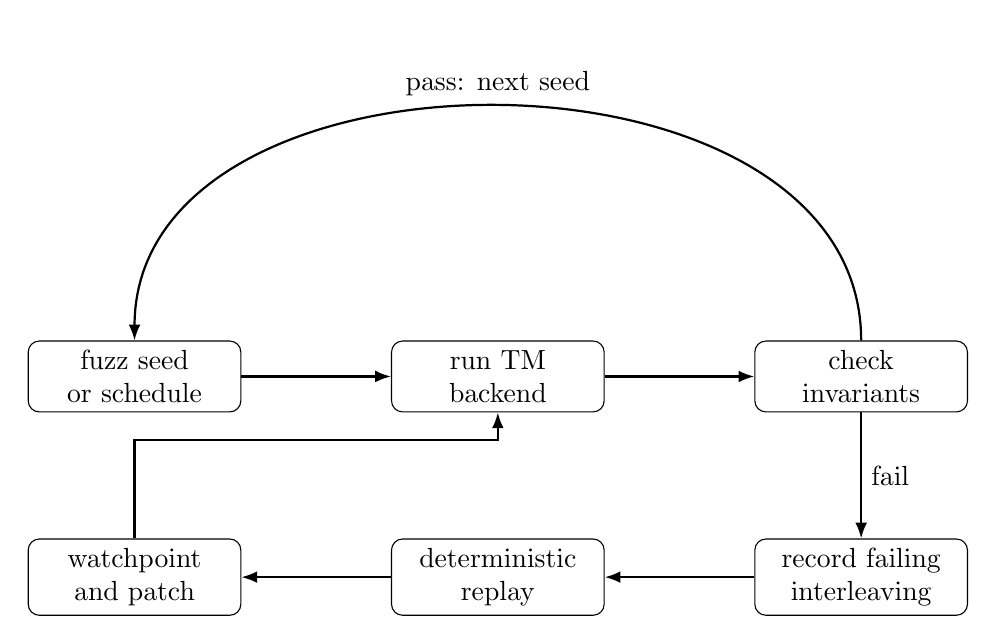
\begin{tikzpicture}[
    node distance=1.6cm and 1.9cm,
    box/.style={draw, rounded corners, align=center, minimum width=2.7cm, minimum height=0.9cm},
    arrow/.style={-{Latex[length=2mm]}, thick}
]
\node[box] (seed) {fuzz seed\\or schedule};
\node[box, right=of seed] (run) {run TM\\backend};
\node[box, right=of run] (check) {check\\invariants};
\node[box, below=of check] (record) {record failing\\interleaving};
\node[box, left=of record] (replay) {deterministic\\replay};
\node[box, left=of replay] (fix) {watchpoint\\and patch};

\draw[arrow] (seed) -- (run);
\draw[arrow] (run) -- (check);
\draw[arrow] (check) -- node[right]{fail} (record);
\draw[arrow] (record) -- (replay);
\draw[arrow] (replay) -- (fix);
\draw[arrow] (fix) |- ($(run.south)+(0,-0.35)$) -- (run.south);
\draw[arrow] (check.north) to[out=90,in=90,looseness=1.1] node[above]{pass: next seed} (seed.north);
\end{tikzpicture}
\caption{A TM debugging loop: random or systematic exploration finds a failing interleaving; replay makes the failure local enough to debug.}
\label{fig:tm-debugging-loop}
\end{figure}

\section{Worked Example: Replay of a Lost-Update}
\index{deterministic scheduling}\index{replay}
\label{sec:replay-lost-update}

The next program is deliberately not a correct TM implementation. It is a minimal deterministic scheduler that reproduces a money-conservation failure by forcing a particular interleaving. Each account is atomic to avoid undefined behavior in the C++ memory model; the bug is logical non-atomicity, not a data race.

\begin{lstlisting}[language=C++, caption={A deterministic replay schedule that exposes a non-atomic transfer.}]
#include <atomic>
#include <cassert>
#include <condition_variable>
#include <iostream>
#include <mutex>
#include <thread>
#include <utility>
#include <vector>

class Replay {
public:
    explicit Replay(std::vector<std::pair<int, int> > script)
        : script_(std::move(script)), pos_(0) {}

    void checkpoint(int tid, int step) {
        std::unique_lock<std::mutex> lk(mu_);
        cv_.wait(lk, [&] {
            return pos_ < script_.size()
                && script_[pos_] == std::make_pair(tid, step);
        });
        ++pos_;
        cv_.notify_all();
    }

private:
    std::vector<std::pair<int, int> > script_;
    std::size_t pos_;
    std::mutex mu_;
    std::condition_variable cv_;
};

struct Bank {
    std::atomic<int> a{100};
    std::atomic<int> b{100};
};

static void nonatomic_transfer(Bank& bank, Replay& replay,
                               int tid, int amount) {
    replay.checkpoint(tid, 0);
    int old_a = bank.a.load();

    replay.checkpoint(tid, 1);
    int old_b = bank.b.load();

    replay.checkpoint(tid, 2);
    bank.a.store(old_a - amount);

    replay.checkpoint(tid, 3);
    bank.b.store(old_b + amount);
}

int main() {
    Bank bank;

    /*
       T0 debits A, T1 observes that debit, T1 credits B,
       then T0 overwrites B with an older value.
    */
    Replay replay({
        {0, 0}, {0, 1}, {0, 2},
        {1, 0}, {1, 1}, {1, 2}, {1, 3},
        {0, 3}
    });

    std::thread t0(nonatomic_transfer, std::ref(bank),
                   std::ref(replay), 0, 10);
    std::thread t1(nonatomic_transfer, std::ref(bank),
                   std::ref(replay), 1, 20);

    t0.join();
    t1.join();

    const int final_sum = bank.a.load() + bank.b.load();

    assert(bank.a.load() == 70);
    assert(bank.b.load() == 110);
    assert(final_sum == 180);

    std::cout << "replayed invariant failure: sum = "
              << final_sum << "\n";
    return 0;
}
\end{lstlisting}

\begin{itemize}
    \item The schedule is the test case. Once recorded, the failure is no longer a Heisenbug.
    \item Atomics remove undefined behavior from the demonstration; they do not provide transaction atomicity.
    \item A watchpoint on \texttt{bank.b} identifies the overwrite: thread 0 writes a value computed before thread 1's credit.
    \item A real TM backend prevents this execution by locking, validating, versioning, or aborting one transaction.
\end{itemize}

\section{Summary}
\begin{itemize}
    \item Debugging concurrent TM code requires tools that can replay rare interleavings.
    \item Systematic testing can expose Heisenbugs that appear only under specific schedules.
    \item Invariant tests are most useful when they are backend-independent: the same bank, counter, or data-structure oracle should run against SGL, TL2, NOrec, TinySTM variants, SwissTM, persistent backends, distributed backends, and GPU designs.
    \item The companion implementation uses both concrete tests and abstract specifications: the concrete suites check transactional and data-structure behavior, while TLA+ specifications check protocol-level safety.
\end{itemize}

\section{Exercises}
\begin{enumerate}
    \item Design a fuzzing strategy that randomly injects aborts to stress-test a TM's undo-log correctness.
    \item Given a recorded \texttt{rr} trace where a transaction T commits but its writes never appear, hypothesise where to set a watchpoint and how to step backwards to find the bug.
    \item A deterministic scheduler explores interleavings with a bounded number of preemptions. Explain how this bound trades off completeness for tractability.
    \item \emph{[implementation]} Extend Listing~\ref{sec:abort-fuzz-bank}'s harness with account floors: no committed transaction may leave an account below zero. Keep money conservation as a separate invariant, and report which invariant fails first.
    \item \emph{[verification]} Write a two-account TLA+ model of transfer with actions \textsc{Read}, \textsc{Debit}, \textsc{Credit}, \textsc{Commit}, and \textsc{Abort}. Add the money-conservation invariant and then intentionally omit rollback for \textsc{Debit}; confirm that the model checker finds a counterexample.
    \item \emph{[theory]} Bounded-preemption testing often finds bugs with a small bound. Give one reason this empirical fact is plausible for TM implementations, and one class of TM bug that may require a larger bound or a different exploration strategy.
\end{enumerate}

% -------------------------------------------------------------------
\chapter{Pitfalls – Memory, Signals, and Optimizations}
\section{Memory Management: malloc and free}
\begin{itemize}
    \item Speculative allocation: memory allocated inside a transaction must be freed on abort.
    \item Deferred freeing: a free executed inside a transaction cannot be released until commit.
    \item Balanced‑free taxonomy and practical implementations.
    \item Speculative-allocations list: allocations tracked per transaction and rolled back on abort.
    \item The double-free trap: a region allocator reusing addresses across transactions makes a naive double-free detector fire on legitimate reuse.
    \item Deferred-free sets: freed pointers held until commit; visible to other transactions via the read path.
    \item TM-aware memory allocators (region vs.\ general-purpose) and the interaction with stack-address checks.
\end{itemize}

\begin{table}[htbp]
\centering
 \begin{tabular}{|p{0.22\linewidth}|p{0.24\linewidth}|p{0.22\linewidth}|p{0.22\linewidth}|}
\hline
\textbf{Operation} & \textbf{When executed} & \textbf{Abort action} & \textbf{Commit action} \\
\hline
\texttt{malloc} outside transaction &
Immediately visible &
None &
None \\
\hline
\texttt{malloc} inside transaction &
Recorded in speculative list &
Release allocation &
Publish by forgetting log entry \\
\hline
\texttt{free} outside transaction &
Immediately releases memory &
None &
None \\
\hline
\texttt{free} inside transaction &
Recorded in deferred-free set &
Forget deferred free &
Release after commit point \\
\hline
Region reuse &
May recycle same address &
Generation or ownership check &
Generation advances with region \\
\hline
\end{tabular}
\caption{Transactional allocation and freeing rules.  The key asymmetry is that speculative allocations are undone on abort, while transactional frees are delayed until commit.}
\label{tab:tx-memory-rules}
\end{table}

\section{Worked Example: Deferred Free in a Bank Transfer}
\index{deferred free}\index{speculative allocation}\index{money conservation}
\label{sec:deferred-free-bank-example}

The allocator wrapper below is deliberately small.  It shows the two lists every
real implementation needs: allocations made by the current transaction, and
pointers whose \texttt{free} must be deferred until the transaction commits.
The transfer body allocates an audit record speculatively.  On abort, the record
is released.  On commit, ownership of the record passes to the log.

\begin{lstlisting}[language=C, caption={A minimal transactional allocation wrapper for a bank transfer.}]
#include <assert.h>
#include <stdbool.h>
#include <stdio.h>
#include <stdlib.h>

enum { NACC = 2, FLOOR = 0 };

typedef struct Account {
    int balance;
} Account;

typedef struct Audit {
    int from;
    int to;
    int amount;
    struct Audit *next;
} Audit;

typedef struct PtrNode {
    void *ptr;
    struct PtrNode *next;
} PtrNode;

typedef struct Tx {
    PtrNode *allocs;        /* allocations to free on abort */
    PtrNode *deferred;      /* frees to perform on commit    */
    bool active;
} Tx;

static Audit *audit_log = NULL;

static void push_ptr(PtrNode **head, void *ptr) {
    PtrNode *n = (PtrNode *)malloc(sizeof(*n));
    assert(n != NULL);
    n->ptr = ptr;
    n->next = *head;
    *head = n;
}

static bool remove_ptr(PtrNode **head, void *ptr) {
    PtrNode **cur = head;
    while (*cur != NULL) {
        if ((*cur)->ptr == ptr) {
            PtrNode *dead = *cur;
            *cur = dead->next;
            free(dead);
            return true;
        }
        cur = &(*cur)->next;
    }
    return false;
}

static void free_ptr_list(PtrNode **head, bool free_payload) {
    while (*head != NULL) {
        PtrNode *n = *head;
        *head = n->next;
        if (free_payload) {
            free(n->ptr);
        }
        free(n);
    }
}

static void tx_begin(Tx *tx) {
    tx->allocs = NULL;
    tx->deferred = NULL;
    tx->active = true;
}

static void *tx_malloc(Tx *tx, size_t nbytes) {
    void *p = malloc(nbytes);
    assert(p != NULL);
    if (tx->active) {
        push_ptr(&tx->allocs, p);
    }
    return p;
}

static void tx_free(Tx *tx, void *ptr) {
    if (ptr == NULL) {
        return;
    }

    /*
     * If the pointer was allocated by this transaction, freeing it cancels the
     * speculative allocation.  Otherwise the free is delayed until commit.
     */
    if (tx->active && remove_ptr(&tx->allocs, ptr)) {
        free(ptr);
    } else if (tx->active) {
        push_ptr(&tx->deferred, ptr);
    } else {
        free(ptr);
    }
}

static void tx_abort(Tx *tx) {
    assert(tx->active);
    free_ptr_list(&tx->allocs, true);    /* undo speculative allocations */
    free_ptr_list(&tx->deferred, false); /* do not free old objects       */
    tx->active = false;
}

static void tx_commit(Tx *tx) {
    assert(tx->active);
    free_ptr_list(&tx->allocs, false);   /* allocations become ordinary  */
    free_ptr_list(&tx->deferred, true);  /* now old objects can be freed */
    tx->active = false;
}

static bool transfer(Tx *tx, Account a[NACC], int from, int to, int amount) {
    tx_begin(tx);

    Audit *rec = (Audit *)tx_malloc(tx, sizeof(*rec));
    rec->from = from;
    rec->to = to;
    rec->amount = amount;

    if (a[from].balance - amount < FLOOR) {
        tx_abort(tx);
        return false;
    }

    a[from].balance -= amount;
    a[to].balance += amount;

    rec->next = audit_log;
    audit_log = rec;

    tx_commit(tx);
    return true;
}

int main(void) {
    Account a[NACC] = { {100}, {50} };
    Tx tx;

    int before = a[0].balance + a[1].balance;
    bool ok = transfer(&tx, a, 0, 1, 25);
    int after = a[0].balance + a[1].balance;

    assert(ok);
    assert(a[0].balance >= FLOOR);
    assert(a[1].balance >= FLOOR);
    assert(before == after);
    assert(audit_log != NULL && audit_log->amount == 25);

    tx_free(&tx, audit_log);
    audit_log = NULL;
    return 0;
}
\end{lstlisting}

\begin{itemize}
    \item Speculative allocation is private until commit; abort must release it.
    \item A transactional \texttt{free} is not a memory reclamation event.  It is a commit action.
    \item The bank invariant is independent of allocation policy, but the audit record's lifetime is not.
    \item A production TM also needs validation: another transaction must not read an object after its freeing transaction commits.
\end{itemize}

\begin{figure}[htbp]
\centering
\resizebox{\textwidth}{!}{%
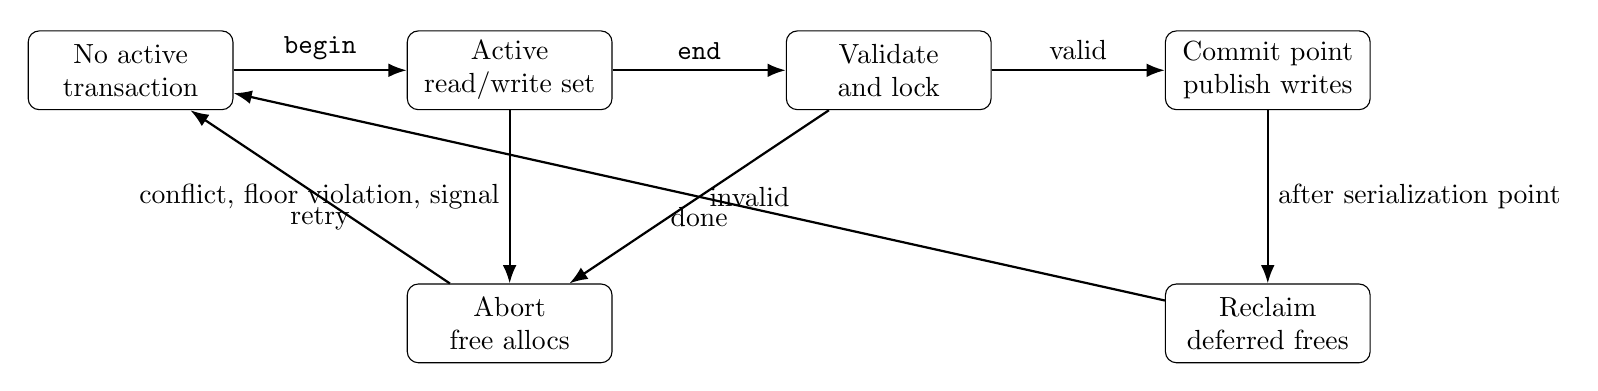
\begin{tikzpicture}[
    node distance=2.2cm,
    state/.style={draw, rounded corners, align=center, minimum width=2.6cm, minimum height=1.0cm},
    arrow/.style={-Latex, thick}
]
\node[state] (idle) {No active\\transaction};
\node[state, right=of idle] (active) {Active\\read/write set};
\node[state, below=of active] (abort) {Abort\\free allocs};
\node[state, right=of active] (validate) {Validate\\and lock};
\node[state, right=of validate] (commit) {Commit point\\publish writes};
\node[state, below=of commit] (reclaim) {Reclaim\\deferred frees};

\draw[arrow] (idle) -- node[above]{\texttt{begin}} (active);
\draw[arrow] (active) -- node[left]{conflict, floor violation, signal} (abort);
\draw[arrow] (abort) -- node[below]{retry} (idle);
\draw[arrow] (active) -- node[above]{\texttt{end}} (validate);
\draw[arrow] (validate) -- node[above]{valid} (commit);
\draw[arrow] (validate) -- node[right]{invalid} (abort);
\draw[arrow] (commit) -- node[right]{after serialization point} (reclaim);
\draw[arrow] (reclaim) -- node[below]{done} (idle);
\end{tikzpicture}%
}
\caption{Resource state machine for a software transaction.  Allocations are reclaimed on abort; frees are reclaimed only after the commit point.}
\label{fig:tx-resource-state}
\end{figure}

\section{Signal Safety and \texttt{sigsetjmp}/\texttt{longjmp}}
\begin{itemize}
    \item The stack‑corruption hazard: \texttt{begin} inside a function, function returns, abort jumps to corrupted frame.
    \item Alternate signal stacks and safe checkpointing strategies.
    \item The DATA-symbol subtlety: the runtime exports \texttt{tm\_sigsetjmp}/\texttt{tm\_longjmp} as function pointers, not functions --- a DATA/TEXT symbol collision with a compiler-generated direct call is a classic segfault (fixed in the companion repo, and instructive).
    \item TLS vs.\ stack jmp buffers: keeping the retry buffer in thread-local storage so it outlives any single frame.
\end{itemize}

\subsection{The Conservative Signal-Safety Policy}
\index{signal safety}
Because the frame-lifetime hazard is \emph{ubiquitous} (it is hidden inside
\texttt{tm\_begin}/\texttt{tm\_end}), the book adopts a single, conservative
policy instead of a list of exceptions:

\begin{itemize}
    \item \textbf{Allowed inside a transaction:} transactional reads and writes, transactional allocation (\texttt{tm\_malloc}), and the retry loop itself --- everything that stays within the runtime's metadata.
    \item \textbf{Forbidden:} any \texttt{sigsetjmp} whose frame may outlive the transaction; blocking signals that the runtime's \texttt{tm\_sigsetjmp} wraps; and hand-written \texttt{siglongjmp} to a stack buffer.
    \item \textbf{Must abort or become irrevocable:} operations with externally visible side effects (I/O, syscalls) that cannot be undone; these force a fallback to a serializing path (Ch.~8) before the operation runs.
    \item The policy is a property the TLA+ models do \emph{not} check: the models abstract the retry mechanism away entirely (Part~III), so frame validity is enforced by convention plus TLS re-arming --- not by the checker.
\end{itemize}

\section{Worked Example: The Frame-Lifetime Hazard}
\index{sigsetjmp}\index{siglongjmp}\index{TLS jmp buffer}\index{retry loop}\index{abort}\index{sandboxing}\index{privatization}
\label{sec:jmpbuf-example}

Why \texttt{sigsetjmp} inside a returning function is a corruption bomb ---
the retry-loop primitive of \S\ref{sec:api-example} hides this:

\begin{lstlisting}[language=C, caption={A transaction that outlives its own frame.}]
void helper(int *a, int *b, int n) {
    tm_begin();                     /* sigsetjmp saves THIS frame */
    transfer_body(a, b, n);         /* may longjmp on abort       */
    tm_end();
}                                   /* frame now dead             */

void worker() {
    helper(a, b, n);                /* returns; jmpbuf is stale   */
    /* ... later, an abort longjmps back into helper's dead frame */
}
\end{lstlisting}

\begin{itemize}
    \item The saved context points into \texttt{helper}'s stack frame, which is gone the moment \texttt{helper} returns.
    \item The standard fix is the bullet above: keep the \texttt{jmp\_buf} in TLS and re-arm it on every attempt, so the retry target is never a dead frame.
    \item The DATA-symbol subtlety of this chapter is the other half: the runtime exports \texttt{tm\_sigsetjmp} as a function pointer, and a compiler that emits a direct call jumps to the pointer variable's address --- a classic segfault the companion repo fixed.
    \item Exercise~2 of this chapter asks you to design the runtime change precisely.
\end{itemize}

\section{Worked Example: TLS Retry Buffer}
\index{TLS jmp buffer}\index{retry loop}\index{abort}
\label{sec:tls-retry-buffer-example}

A safe retry loop stores the checkpoint in thread-local runtime state, not in a
caller-owned object.  The following program is small enough to compile, but it
captures the important rule: every attempt re-arms the TLS buffer before
running the transactional body.

\begin{lstlisting}[language=C, caption={A TLS retry buffer re-armed on each attempt.}]
#include <assert.h>
#include <setjmp.h>
#include <stdbool.h>
#include <stdio.h>

enum { NACC = 2, FLOOR = 0 };

typedef struct Account {
    int balance;
} Account;

typedef struct TxTLS {
    jmp_buf retry;
    bool armed;
    int attempts;
} TxTLS;

static _Thread_local TxTLS tm_tls;

static int tm_begin(void) {
    tm_tls.armed = true;
    tm_tls.attempts++;
    return setjmp(tm_tls.retry);
}

static void tm_abort(void) {
    assert(tm_tls.armed);
    longjmp(tm_tls.retry, 1);
}

static void tm_end(void) {
    tm_tls.armed = false;
}

static void transfer_body(Account a[NACC], int from, int to, int amount) {
    if (a[from].balance - amount < FLOOR) {
        tm_abort();
    }
    a[from].balance -= amount;
    a[to].balance += amount;
}

static bool transfer_retry(Account a[NACC], int from, int to, int amount) {
    for (;;) {
        int aborted = tm_begin();
        if (aborted) {
            tm_end();
            return false;
        }

        transfer_body(a, from, to, amount);
        tm_end();
        return true;
    }
}

int main(void) {
    Account a[NACC] = { {100}, {50} };

    int before = a[0].balance + a[1].balance;
    bool ok = transfer_retry(a, 0, 1, 25);
    int after = a[0].balance + a[1].balance;

    assert(ok);
    assert(before == after);
    assert(a[0].balance == 75);
    assert(a[1].balance == 75);

    before = a[0].balance + a[1].balance;
    ok = transfer_retry(a, 0, 1, 1000);
    after = a[0].balance + a[1].balance;

    assert(!ok);
    assert(before == after);
    return 0;
}
\end{lstlisting}

\begin{itemize}
    \item The retry buffer has thread lifetime; it is not tied to the helper function that called \texttt{tm\_begin}.
    \item Re-arming is per attempt.  Reusing an old checkpoint after commit is a bug.
    \item The example returns \texttt{false} after one failed attempt to keep the program finite; a real TM retry loop may back off and retry.
    \item The code still does not make arbitrary signal handlers safe.  It only fixes the lifetime of the transaction's own retry target.
\end{itemize}

\section{Compiler Optimizations Revisited}
\begin{itemize}
    \item Dead‑store elimination, LICM, CSE, barrier hoisting – concrete bug examples.
    \item Intrinsics and annotations to protect transactional regions.
    \item Crossing the barrier: an optimizer that hoists a transactional load above the instrumentation call observes a state no valid execution has.
    \item The rule of thumb: transactional memory accesses are special function calls, not plain loads; optimizing through them requires their side effects to be declared.
\end{itemize}

\section{Worked Example: Preventing Barrier Hoisting}
\index{compiler optimization}\index{barrier hoisting}\index{transactional load}\index{opacity}
\label{sec:barrier-hoisting-example}

This example is not a full STM.  It is the compiler contract in isolation.
The wrappers are marked \texttt{noinline}, touch unknown memory, and contain a
compiler barrier.  That is enough to prevent ordinary scalar optimizations from
turning transactional accesses into plain loads and stores.

\begin{lstlisting}[language=C, caption={Transactional access wrappers with an explicit compiler barrier.}]
#include <assert.h>
#include <stdbool.h>
#include <stdint.h>

typedef struct Account {
    int balance;
} Account;

typedef struct Tx {
    unsigned reads;
    unsigned writes;
} Tx;

static void compiler_barrier(void) {
#if defined(__GNUC__) || defined(__clang__)
    __asm__ __volatile__("" ::: "memory");
#endif
}

__attribute__((noinline))
static int tm_read_int(Tx *tx, const int *addr) {
    compiler_barrier();
    tx->reads++;
    int value = *addr;
    compiler_barrier();
    return value;
}

__attribute__((noinline))
static void tm_write_int(Tx *tx, int *addr, int value) {
    compiler_barrier();
    tx->writes++;
    *addr = value;
    compiler_barrier();
}

static bool transfer_tx(Tx *tx, Account *from, Account *to, int amount) {
    int from_balance = tm_read_int(tx, &from->balance);
    int to_balance = tm_read_int(tx, &to->balance);

    if (from_balance < amount) {
        return false;
    }

    tm_write_int(tx, &from->balance, from_balance - amount);
    tm_write_int(tx, &to->balance, to_balance + amount);
    return true;
}

int main(void) {
    Account a = {100};
    Account b = {50};
    Tx tx = {0, 0};

    int before = a.balance + b.balance;
    bool ok = transfer_tx(&tx, &a, &b, 25);
    int after = a.balance + b.balance;

    assert(ok);
    assert(before == after);
    assert(a.balance == 75);
    assert(b.balance == 75);
    assert(tx.reads == 2);
    assert(tx.writes == 2);
    return 0;
}
\end{lstlisting}

\begin{itemize}
    \item Transactional reads and writes are observable operations of the runtime, even when the accessed object is an ordinary \texttt{int}.
    \item Hoisting \texttt{from->balance} above \texttt{tm\_read\_int} skips validation and may observe a value that is not opaque.
    \item Eliminating the second read because a prior store appears to dominate it is only legal if the compiler also proves the TM metadata effects are preserved.
    \item Production systems encode this contract with intrinsics, ABI rules, opaque calls, volatile metadata accesses, or compiler passes that understand transactions.
\end{itemize}

\section{Summary}
\begin{itemize}
    \item A robust TM must handle resource management and OS interactions that break naive transactional boundaries.
    \item Many pitfalls arise from the impedance mismatch between transactional semantics and low‑level system mechanisms.
    \item Each pitfall has a canonical fix: deferred frees, TLS jmp buffers, and side-effect declarations.
\end{itemize}

\section{Exercises}
\begin{enumerate}
    \item A transaction allocates a linked list node, then aborts. Explain why a simple \texttt{free} is unsafe if another thread read a pointer to that node before the abort.
    \item \texttt{sigsetjmp} saves the stack context. If a transaction begins inside function \texttt{f} and \texttt{f} returns before the transaction commits, explain exactly why a later abort jumps to a corrupted stack frame. Propose a runtime change that prevents this.
    \item An optimizer eliminates a load inside a transaction because it sees a preceding store to the same address. Under what circumstances could this break opacity?
    \item \emph{[implementation]} Extend the allocator wrapper in \S\ref{sec:deferred-free-bank-example} with a generation number per allocation.  Show how the generation prevents a naive double-free detector from rejecting legitimate address reuse by a region allocator.
    \item \emph{[verification]} Write a small TLA+ or PlusCal model of the state machine in Fig.~\ref{fig:tx-resource-state}.  Include two accounts, one transfer operation, an abort action, and invariants for account floors and money conservation.
    \item \emph{[theory]} Give a precise compiler-side condition under which common-subexpression elimination of two transactional reads from the same address is semantics-preserving.  Your answer must mention validation, intervening writes, and opacity.
\end{enumerate}

\chapter{Performance Modeling and Tuning}

\section{Metrics and Benchmarks}
\begin{itemize}
    \item Throughput, abort rate, wasted work.
    \item The STAMP benchmark suite.
    \item Secondary metrics: occupancy/parallelism, speedup over SGL, energy under contention.
    \item Abort rate alone is misleading: wasted work, measured as restarts times lost progress, and commit latency matter more.
    \item STAMP's eight kernels are \texttt{bayes}, \texttt{genome}, \texttt{intruder}, \texttt{kmeans}, \texttt{labyrinth}, \texttt{ssca2}, \texttt{vacation}, and \texttt{yada}. They stress read-heavy, write-heavy, long, and tree/graph-shaped accesses.
    \item Microbenchmarks such as counter, bank, and linked-list isolate controlled parameter sweeps.
\end{itemize}

\section{Analytical Models}
\label{sec:perf-analytical}
\begin{itemize}
    \item Markov chain models of contention.
    \item Applying queueing theory and Little's Law to predict performance:
    $$
    L = \lambda W
    $$
    where \(L\) is the mean number of in-flight transactions, \(\lambda\) is committed throughput, and \(W\) is mean transaction latency.
    \item The expected-retries model: if each attempt aborts independently with probability
    $$
    p_{\mathrm{abort}},
    $$
    then the mean attempts per committed transaction is
    $$
    E[\mathrm{attempts\ per\ commit}] =
    \frac{1}{1-p_{\mathrm{abort}}}.
    $$
    This scaling breaks down under high contention because attempts are not independent and because retries change cache residency and queueing delay.
    \item Cost-per-operation models decompose begin/read/write/commit cycle counts and calibrate them against real runs. This is the machine-profile approach used by the companion simulator.
    \item The model holds when conflicts are approximately independent and the working set fits the relevant cache level. It misses memory-hierarchy effects, coherence storms, and cache-line false conflicts.
\end{itemize}

\begin{figure}[htbp]
\centering
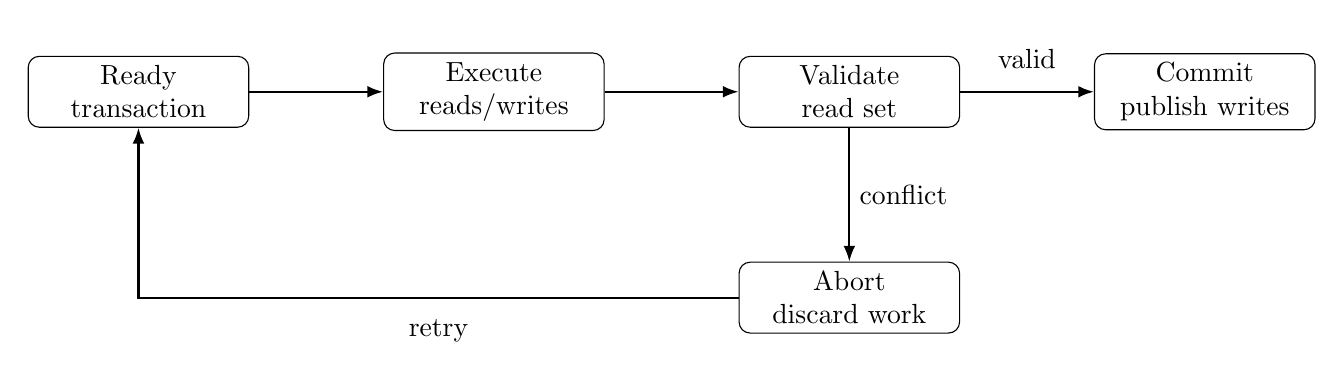
\begin{tikzpicture}[
    node distance=1.7cm,
    every node/.style={draw, rounded corners, align=center, minimum width=2.8cm, minimum height=0.8cm},
    arrow/.style={-{Latex[length=2mm]}, thick}
]
\node (ready) {Ready\\transaction};
\node[right=of ready] (execute) {Execute\\reads/writes};
\node[right=of execute] (validate) {Validate\\read set};
\node[right=of validate] (commit) {Commit\\publish writes};
\node[below=of validate] (abort) {Abort\\discard work};

\draw[arrow] (ready) -- (execute);
\draw[arrow] (execute) -- (validate);
\draw[arrow] (validate) -- node[above, draw=none, minimum width=0cm] {valid} (commit);
\draw[arrow] (validate) -- node[right, draw=none, minimum width=0cm] {conflict} (abort);
\draw[arrow] (abort.west) -| node[pos=0.25, below, draw=none, minimum width=0cm] {retry} (ready.south);
\end{tikzpicture}
\caption{A minimal performance state machine for optimistic TM. Throughput counts transitions into commit; abort rate counts transitions into abort; wasted work is the time spent in execute before an abort.}
\label{fig:perf-state-machine}
\end{figure}

\section{Experimental Methodology}
\begin{itemize}
    \item Profiling with \texttt{perf}; avoiding warm-up and noise pitfalls.
    \item Warm-up, result stabilization, and outlier rejection.
    \item Comparing against the uninstrumented baseline, not just against other TMs: instrumentation cost must be separated from algorithm cost.
    \item Benchmark hygiene: pin threads, disable frequency scaling, report variance, and use enough repetitions to make five percent differences meaningful.
    \item Reproducibility: record machine profile, toolchain, and configuration alongside every measurement.
\end{itemize}

\begin{table}[htbp]
\centering
\caption{Measured anchors from the companion M1 Pro fuzz/bank runs. These are calibration points, not universal rankings.}
\label{tab:perf-anchors}
\begin{tabular}{p{0.15\linewidth}p{0.19\linewidth}p{0.23\linewidth}p{0.31\linewidth}}
\hline
Backend & Workload slice & Throughput & Modeling use \\
\hline
NOrec-BF & read-mostly & about 829K txns/s & Bloom-filtered read-set cost \\
NOrec & read-mostly & about 553K txns/s & global-clock validation cost \\
TL2 & fuzz/bank & about 2.06M txns/s & ownership-record fast path \\
TSC-TM & fuzz/bank & about 2.05M txns/s & timestamp fast path \\
MVLog & write-heavy & about 275K txns/s & multi-version log pressure \\
MVLog & read-mostly & about 109K txns/s & multi-version read overhead \\
\hline
\end{tabular}
\end{table}

\section{Worked Example: Measuring Attempts in the Bank Benchmark}
\index{bank benchmark}\index{single global lock}\index{wasted work}
\label{sec:perf-bank-attempts}

This standalone C++17 program implements the bank benchmark with a single
global lock. It is intentionally simple: the point is to produce a clean
baseline for throughput, attempts, semantic rejects, and the money-conservation
invariant before replacing the critical section by NOrec, TL2, TinySTM, or
another backend.

\begin{lstlisting}[language=C++, caption={A compilable SGL bank benchmark that reports attempts and checks conservation.}]
#include <atomic>
#include <chrono>
#include <cstdint>
#include <cstdlib>
#include <iostream>
#include <mutex>
#include <random>
#include <thread>
#include <vector>

struct Account {
    long long balance;
};

struct Stats {
    std::uint64_t attempts = 0;
    std::uint64_t commits = 0;
    std::uint64_t rejects = 0;
};

static bool transfer_sgl(std::vector<Account>& bank,
                         std::mutex& global_lock,
                         std::size_t from,
                         std::size_t to,
                         long long amount,
                         long long floor,
                         Stats& stats) {
    ++stats.attempts;

    std::lock_guard<std::mutex> guard(global_lock);

    if (from == to) {
        ++stats.commits;
        return true;
    }

    if (bank[from].balance - amount < floor) {
        ++stats.rejects;          // semantic reject, not a TM conflict
        return false;
    }

    bank[from].balance -= amount;
    bank[to].balance += amount;
    ++stats.commits;
    return true;
}

int main(int argc, char** argv) {
    const std::size_t threads =
        argc > 1 ? static_cast<std::size_t>(std::strtoull(argv[1], nullptr, 10)) : 4;
    const std::size_t accounts =
        argc > 2 ? static_cast<std::size_t>(std::strtoull(argv[2], nullptr, 10)) : 64;
    const int seconds =
        argc > 3 ? std::atoi(argv[3]) : 2;

    const long long initial_balance = 1000;
    const long long floor = 0;
    const long long amount = 1;

    std::vector<Account> bank(accounts, Account{initial_balance});
    const long long initial_total =
        static_cast<long long>(accounts) * initial_balance;

    std::mutex global_lock;
    std::atomic<bool> stop{false};
    std::vector<Stats> per_thread(threads);
    std::vector<std::thread> workers;

    auto start = std::chrono::steady_clock::now();

    for (std::size_t tid = 0; tid < threads; ++tid) {
        workers.emplace_back([&, tid] {
            std::mt19937_64 rng(0xC0FFEEULL + tid);
            std::uniform_int_distribution<std::size_t> pick(0, accounts - 1);

            while (!stop.load(std::memory_order_relaxed)) {
                std::size_t from = pick(rng);
                std::size_t to = pick(rng);
                transfer_sgl(bank, global_lock, from, to,
                             amount, floor, per_thread[tid]);
            }
        });
    }

    std::this_thread::sleep_for(std::chrono::seconds(seconds));
    stop.store(true, std::memory_order_relaxed);

    for (auto& t : workers) {
        t.join();
    }

    auto end = std::chrono::steady_clock::now();
    double elapsed =
        std::chrono::duration<double>(end - start).count();

    std::uint64_t attempts = 0;
    std::uint64_t commits = 0;
    std::uint64_t rejects = 0;
    for (const Stats& s : per_thread) {
        attempts += s.attempts;
        commits += s.commits;
        rejects += s.rejects;
    }

    long long final_total = 0;
    for (const Account& a : bank) {
        final_total += a.balance;
        if (a.balance < floor) {
            std::cerr << "floor violation\n";
            return 2;
        }
    }

    if (final_total != initial_total) {
        std::cerr << "money conservation violation\n";
        return 3;
    }

    std::cout << "threads=" << threads
              << " accounts=" << accounts
              << " commits=" << commits
              << " attempts=" << attempts
              << " rejects=" << rejects
              << " txns_per_sec=" << commits / elapsed
              << " attempts_per_commit="
              << (commits == 0 ? 0.0 : static_cast<double>(attempts) / commits)
              << "\n";

    return 0;
}
\end{lstlisting}

\begin{itemize}
    \item SGL has no speculative conflict aborts. Any reject in this program is caused by the account floor, not by validation failure.
    \item The invariant check is part of the benchmark, not a debugging afterthought. A fast run that loses money is not a performance result.
    \item The same driver shape can wrap a TM backend: keep the random stream, account count, transfer amount, and invariant checks fixed, then replace only the transaction boundary and memory-access API.
    \item Attempts per commit is still useful for SGL because it separates useful commits from semantic rejects. For optimistic TM, add a separate counter for validation aborts.
\end{itemize}

\section{Worked Example: Model Checking a Bounded Contention Counter}
\index{TLA+}\index{model checking}\index{contention}
\label{sec:perf-tla-bank}

The next TLA+ module is deliberately small. It models two workers, two
accounts, a single owner slot, bounded attempts, account floors, and money
conservation. It is not a full TM algorithm. It is a sanity model for the
counters used in a performance report: each attempt is either in flight,
committed, or aborted.

\begin{lstlisting}[caption={A bounded TLA+ model for bank attempts, commits, and aborts.}]
---- MODULE BankFloorContention ----
EXTENDS Naturals, TLC

A == {1, 2}
Workers == {1, 2}
InitBal == [i \in A |-> 5]
Floor == 0
Amount == 1
MaxAttempts == 6

VARIABLES bal, owner, attempts, commits, aborts

vars == <<bal, owner, attempts, commits, aborts>>

From(w) == IF w = 1 THEN 1 ELSE 2
To(w) == IF w = 1 THEN 2 ELSE 1

TotalAttempts == attempts[1] + attempts[2]

Init ==
  /\ bal = InitBal
  /\ owner = 0
  /\ attempts = [w \in Workers |-> 0]
  /\ commits = 0
  /\ aborts = 0

Acquire(w) ==
  /\ owner = 0
  /\ TotalAttempts < MaxAttempts
  /\ owner' = w
  /\ attempts' = [attempts EXCEPT ![w] = @ + 1]
  /\ UNCHANGED <<bal, commits, aborts>>

BusyAbort(w) ==
  /\ owner # 0
  /\ owner # w
  /\ TotalAttempts < MaxAttempts
  /\ owner' = owner
  /\ attempts' = [attempts EXCEPT ![w] = @ + 1]
  /\ aborts' = aborts + 1
  /\ UNCHANGED <<bal, commits>>

Finish(w) ==
  LET f == From(w)
      t == To(w)
  IN
    /\ owner = w
    /\ owner' = 0
    /\ IF bal[f] >= Floor + Amount
          THEN /\ bal' = [bal EXCEPT ![f] = @ - Amount,
                                     ![t] = @ + Amount]
               /\ commits' = commits + 1
               /\ aborts' = aborts
          ELSE /\ bal' = bal
               /\ commits' = commits
               /\ aborts' = aborts + 1
    /\ attempts' = attempts

Next ==
  \E w \in Workers:
      Acquire(w) \/ BusyAbort(w) \/ Finish(w)

Spec == Init /\ [][Next]_vars

TypeOK ==
  /\ bal \in [A -> Nat]
  /\ owner \in Workers \cup {0}
  /\ attempts \in [Workers -> Nat]
  /\ commits \in Nat
  /\ aborts \in Nat

MoneyConserved ==
  bal[1] + bal[2] = InitBal[1] + InitBal[2]

Floors ==
  /\ bal[1] >= Floor
  /\ bal[2] >= Floor

AttemptsAccounted ==
  attempts[1] + attempts[2] =
    commits + aborts + (IF owner = 0 THEN 0 ELSE 1)

\* TLC: check SPECIFICATION Spec
\* TLC: check INVARIANTS TypeOK MoneyConserved Floors AttemptsAccounted
====
\end{lstlisting}

\begin{itemize}
    \item The invariant \texttt{AttemptsAccounted} is the accounting identity behind the benchmark columns: an attempt is committed, aborted, or still owned.
    \item The owner slot makes contention explicit. A worker that arrives while another worker owns the slot increments both attempts and aborts.
    \item The money invariant is independent of the performance counters. Do not infer correctness from high throughput.
    \item Bounding attempts makes the state space finite; the same idea is used in larger model-checked specifications for the companion backends.
\end{itemize}

\section{Worked Example: Reading a Benchmark Report}
\index{benchmark}\index{throughput}\index{abort rate}
\label{sec:perf-example}

What Part~III's models and this chapter's methodology look like when filled in
with a real sweep across backends:

\begin{lstlisting}[caption={A protocol for separating instrumentation cost from contention.}]
backend   threads   tx/s       aborts   attempt/tx
--------- -------   --------   -------  ----------
uninstr.  1         8.2M       --       --
NOrec     1         450K       0        1.00
NOrec     4         402K       1.2M     1.08
NOrec     8         313K       3.1M     1.17
TL2       8         298K       3.3M     1.19
SGL       8         210K       0        1.00
\end{lstlisting}

\begin{itemize}
    \item The \texttt{uninstr.} row is the baseline this chapter insists on: instrumentation cost is
    $$
    \frac{8.2\ \mathrm{M}}{450\ \mathrm{K}} \approx 18.2,
    $$
    measured against the uninstrumented backend, not against another TM.
    \item The \texttt{attempt/tx} column is the geometric retry model of \S\ref{sec:perf-analytical} read backwards. At 8 threads, NOrec averages 1.17 attempts per committed transaction, so
    $$
    p_{\mathrm{abort}} \approx 1 - \frac{1}{1.17} \approx 0.15.
    $$
    \item SGL shows the serialisation bottleneck of Part~IV: zero aborts, but throughput below every speculative backend at 8 threads.
    \item Exercise~3 asks for the experiment design; the machine-profile record is what the companion simulator's cost calibration consumes.
\end{itemize}

\section{Summary}
\begin{itemize}
    \item Performance evaluation of TM requires both analytical models and careful empirical measurement.
    \item Throughput must be interpreted with aborts, attempts per commit, latency, and validation cost.
    \item A benchmark report is incomplete unless it records the uninstrumented baseline, machine profile, toolchain, workload parameters, and correctness checks.
\end{itemize}

\section{Exercises}
\begin{enumerate}
    \item Fit a simple Markov model to STAMP’s \texttt{intruder} benchmark and estimate the abort probability that maximizes throughput.
    \item Use Little’s Law to explain why a high abort rate causes a sharp drop in throughput even when the system is not CPU-saturated.
    \item Design an experiment to measure the overhead of TM instrumentation vs. fine-grained locking for a linked list.
    \item \emph{[implementation]} Modify Listing~\ref{sec:perf-bank-attempts}'s benchmark so that it records per-thread latency samples for committed transfers. Report median, 95th percentile, and maximum latency, and explain why the maximum is unstable under contention.
    \item \emph{[verification]} Extend the TLA+ model in \S\ref{sec:perf-tla-bank} with a third worker. Add an invariant stating that the number of in-flight attempts is at most one, and check that money conservation still holds.
    \item \emph{[theory]} Starting from the retry model
    $$
    E[\mathrm{attempts\ per\ commit}] =
    \frac{1}{1-p_{\mathrm{abort}}},
    $$
    derive the predicted committed throughput when each attempt costs a fixed time
    $$
    C_{\mathrm{attempt}}.
    $$
    State two concrete reasons why this prediction fails for TL2 or NOrec under high write contention.
\end{enumerate}

% -------------------------------------------------------------------
%  PART VII: ADVANCED TOPICS
% -------------------------------------------------------------------
\part{Advanced Topics}

% -------------------------------------------------------------------
\chapter{From Source to AST: Lexing and Parsing}

\section{Finite Automata and Lexical Analysis}
\begin{itemize}
    \item Regular expressions as a thinking tool; every regular expression compiles to a deterministic finite automaton (DFA) via the subset construction, and a DFA is exactly what a hand-written lexer \emph{is}.
    \item Hand-written lexer for a tiny language containing \texttt{atomic}, identifiers, and braces.
    \item The classic ``keyword vs.\ identifier'' problem: \texttt{atomic} and \texttt{atomically} share a prefix, so the DFA either gives keywords a dedicated path (Figure~\ref{fig:lexer-dfa}) or checks a reserved-word table after a maximal munch.
\end{itemize}

\begin{figure}[ht]
\centering
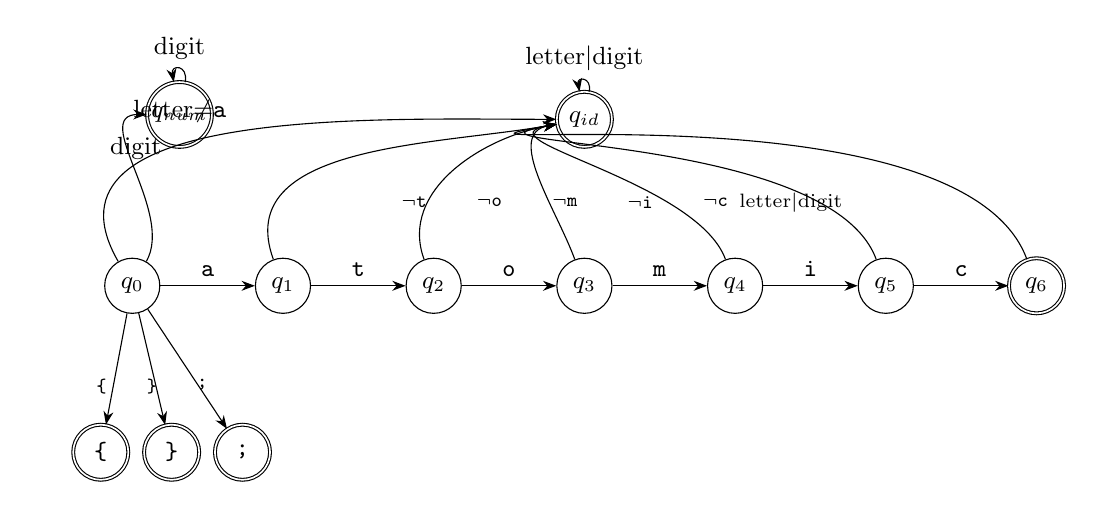
\begin{tikzpicture}[font=\small, node distance=1.5cm]
  \tikzstyle{st}=[circle,draw,inner sep=1pt,minimum size=7mm]
  \tikzstyle{acc}=[circle,draw,double,inner sep=1pt,minimum size=7mm]
  \node[st] (q0) {$q_0$};
  \node[st] (q1) [right=1.2cm of q0] {$q_1$};
  \node[st] (q2) [right=1.2cm of q1] {$q_2$};
  \node[st] (q3) [right=1.2cm of q2] {$q_3$};
  \node[st] (q4) [right=1.2cm of q3] {$q_4$};
  \node[st] (q5) [right=1.2cm of q4] {$q_5$};
  \node[acc] (q6) [right=1.2cm of q5] {$q_6$};
  \node[acc] (qid) [above=1.4cm of q3] {$q_{id}$};
  \node[acc] (qnum) [above=1.4cm of q0,xshift=0.6cm] {$q_{num}$};
  \node[acc] (qlb) [below=1.4cm of q0,xshift=-0.4cm] {\texttt{\char`\{}};
  \node[acc] (qrb) [below=1.4cm of q0,xshift=0.5cm] {\texttt{\char`\}}};
  \node[acc] (qs)  [below=1.4cm of q0,xshift=1.4cm] {\texttt{;}};
  \draw[-{Stealth}] (q0) -- node[above] {\texttt{a}} (q1);
  \draw[-{Stealth}] (q1) -- node[above] {\texttt{t}} (q2);
  \draw[-{Stealth}] (q2) -- node[above] {\texttt{o}} (q3);
  \draw[-{Stealth}] (q3) -- node[above] {\texttt{m}} (q4);
  \draw[-{Stealth}] (q4) -- node[above] {\texttt{i}} (q5);
  \draw[-{Stealth}] (q5) -- node[above] {\texttt{c}} (q6);
  \draw[-{Stealth}] (q0) to[out=120,in=180] node[above left] {letter$\neq$\texttt{a}} (qid);
  \draw[-{Stealth}] (q0) to[out=60,in=-180] node[above] {digit} (qnum);
  \draw[-{Stealth}] (q1) to[out=110,in=190] (qid);
  \draw[-{Stealth}] (q2) to[out=110,in=190] (qid);
  \draw[-{Stealth}] (q3) to[out=110,in=190] (qid);
  \draw[-{Stealth}] (q4) to[out=110,in=190] (qid);
  \draw[-{Stealth}] (q5) to[out=110,in=190] (qid);
  \draw[-{Stealth}] (q6) to[out=110,in=190] (qid);
  \node[font=\scriptsize] at ($(q1)!0.5!(qid)-(0.25,0)$) {$\neg$\texttt{t}};
  \node[font=\scriptsize] at ($(q2)!0.5!(qid)-(0.25,0)$) {$\neg$\texttt{o}};
  \node[font=\scriptsize] at ($(q3)!0.5!(qid)-(0.25,0)$) {$\neg$\texttt{m}};
  \node[font=\scriptsize] at ($(q4)!0.5!(qid)-(0.25,0)$) {$\neg$\texttt{i}};
  \node[font=\scriptsize] at ($(q5)!0.5!(qid)-(0.25,0)$) {$\neg$\texttt{c}};
  \node[font=\scriptsize] at ($(q6)!0.5!(qid)-(0.25,0)$) {letter$\mid$digit};
  \draw[-{Stealth}] (qid) to[out=80,in=100,looseness=4] node[above] {letter$\mid$digit} (qid);
  \draw[-{Stealth}] (qnum) to[out=80,in=100,looseness=4] node[above] {digit} (qnum);
  \draw[-{Stealth}] (q0) -- node[below left,font=\scriptsize] {\texttt{\char`\{}} (qlb);
  \draw[-{Stealth}] (q0) -- node[below,font=\scriptsize] {\texttt{\char`\}}} (qrb);
  \draw[-{Stealth}] (q0) -- node[below right,font=\scriptsize] {\texttt{;}} (qs);
\end{tikzpicture}
\caption{A DFA for the toy lexer. A dedicated path recognizes the keyword \texttt{atomic}; any other continuation falls into the identifier state $q_{id}$, so \texttt{atomically} is an identifier, not a keyword. \texttt{\char`\{}, \texttt{\char`\}}, and \texttt{;} are single-character tokens.}
\label{fig:lexer-dfa}
\end{figure}

\section{Recursive Descent Parsing}
\begin{itemize}
    \item Each grammar rule becomes a function.
    \item Constructing a parse tree / AST for an \texttt{atomic \{ … \}} block.
    \item Why recursive descent is the simplest didactic parsing algorithm.
    \item Its limits: no left recursion, no automatic conflict report, no grammar file --- the grammar lives only in the code.
\end{itemize}

\begin{figure}[htbp]
\centering
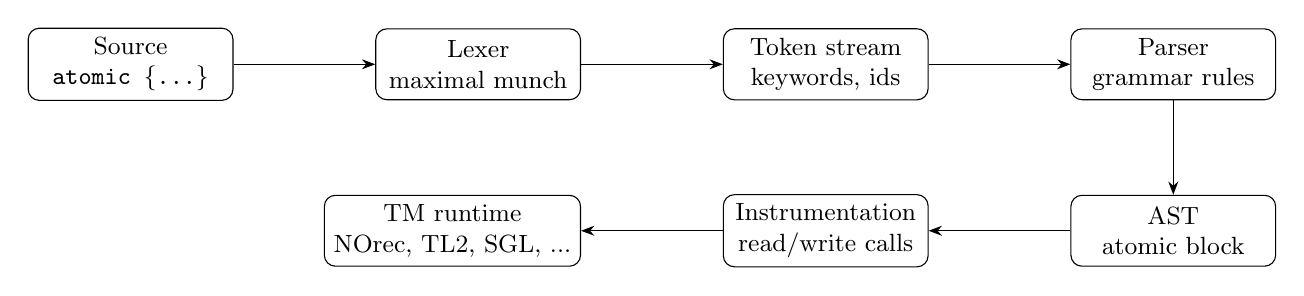
\begin{tikzpicture}[font=\small, node distance=1.8cm]
  \tikzstyle{box}=[draw,rounded corners,align=center,minimum width=2.6cm,minimum height=0.9cm]
  \node[box] (src) {Source\\\texttt{atomic \{...\}}};
  \node[box] (lex) [right=of src] {Lexer\\maximal munch};
  \node[box] (tok) [right=of lex] {Token stream\\keywords, ids};
  \node[box] (parse) [right=of tok] {Parser\\grammar rules};
  \node[box] (ast) [below=1.2cm of parse] {AST\\atomic block};
  \node[box] (ir) [left=of ast] {Instrumentation\\read/write calls};
  \node[box] (rt) [left=of ir] {TM runtime\\NOrec, TL2, SGL, ...};
  \draw[-{Stealth}] (src) -- (lex);
  \draw[-{Stealth}] (lex) -- (tok);
  \draw[-{Stealth}] (tok) -- (parse);
  \draw[-{Stealth}] (parse) -- (ast);
  \draw[-{Stealth}] (ast) -- (ir);
  \draw[-{Stealth}] (ir) -- (rt);
\end{tikzpicture}
\caption{A source-level view of the front-end pipeline. The companion repository instruments at LLVM IR rather than shipping a source-level language, but the logical artifacts are the same: source text becomes tokens, tokens become an AST, and the AST-equivalent control region becomes calls into a concrete TM backend.}
\label{fig:front-end-pipeline}
\end{figure}

\section{Parser Generators: From Yacc to Modern Tools}
\index{parser generator}\index{yacc}\index{bison}\index{LR(0) automaton}\index{ANTLR}\index{tree-sitter}

The most direct answer to ``is Yacc still in use?'' is: yes, and its descendants
are everywhere.  The principle Yacc established --- write the grammar, get a
table-driven parser for free --- is the backbone of countless real compilers,
and the shift-and-reduce automaton it builds is exactly the kind of object
this chapter's automata language can describe.

\begin{itemize}
    \item \emph{Yacc (1975)} compiled a context-free grammar into an \textsc{LALR(1)} parser table; its modern form is \textsc{GNU Bison}, still maintained and still the parser behind many C/C++-adjacent tools (e.g.\ SQL engines, shell grammars).
    \item \emph{The generated automaton is a real object.}  For a simple grammar, the ``parser'' Bison would produce is an LR(0) automaton with one state per set of viable items, as in Figure~\ref{fig:lr0-automaton} for the grammar in Listing~\ref{lst:expr-grammar}.
    \item \emph{Recursive descent you write; an LR table you compute.}  This is the trade-off: hand-written parsers read like the grammar but must avoid left recursion; generated parsers accept the grammar as-is but hide the shift/reduce machinery behind the table.
    \item \emph{Modern tools}.  \textsc{ANTLR} (ALL(*), with Python and many other targets) generates recursive-descent parsers from grammar files; \textsc{tree-sitter} builds error-tolerant, incremental \textsc{GLR} parsers used by editors; Python projects commonly use \textsc{PLY} (a Yacc port), \textsc{SLY} (its successor), or \textsc{Lark} (Earley/LALR from \textsc{EBNF}).
    \item \emph{What this means for transactional constructs}: nothing about \texttt{atomic} is hard to parse --- any of these tools can host the grammar --- so the interesting work stays downstream, in the instrumentation and runtime, where the rest of this book lives.
    \item \emph{Scope note}: this section is a deliberate, self-contained detour. The companion repository instruments at the LLVM-IR level (Chapter~10) and does \emph{not} implement a source-level TM language, so no front-end generator is shipped; the DFA and LR(0) automata here exist to ground the vocabulary (``shift'', ``reduce'', ``item set'') rather than to build a product. Readers who want only the TM pipeline may skip to the worked example.
\end{itemize}

\begin{table}[htbp]
\centering
\begin{tabular}{p{0.20\linewidth}p{0.24\linewidth}p{0.30\linewidth}p{0.16\linewidth}}
\hline
Approach & Parser shape & Strength & Cost \\
\hline
Hand recursive descent & Functions over tokens & Transparent AST construction & No left recursion \\
Yacc/Bison & Table-driven LALR & Compact grammar file & Shift/reduce debugging \\
ANTLR & Generated recursive descent & Rich grammar notation & Toolchain dependency \\
tree-sitter & Incremental GLR & Editor-grade recovery & More machinery \\
\hline
\end{tabular}
\caption{Front-end choices for an \texttt{atomic} construct. The syntax is simple enough for any row; the engineering choice is driven by diagnostics, integration, and maintenance.}
\label{tab:front-end-choices}
\end{table}

\begin{lstlisting}[language={}, caption={A grammar small enough to see the whole automaton, written in Yacc-style BNF.}, label={lst:expr-grammar}]
expr  ::= expr '+' term   |  term
term  ::= id
\end{lstlisting}

\begin{figure}[ht]
\centering
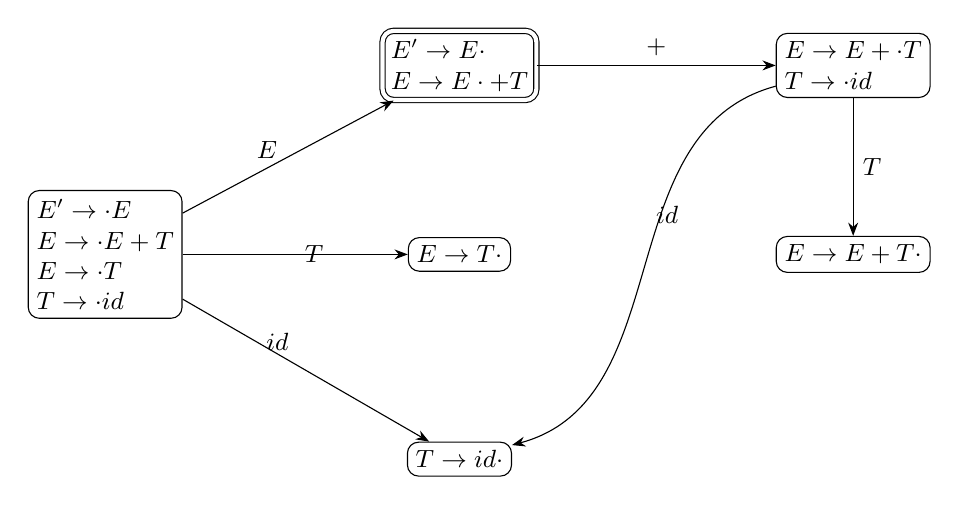
\begin{tikzpicture}[font=\small, node distance=2.6cm]
  \tikzstyle{item}=[rounded corners,draw,inner sep=3pt,align=left]
  \node[item] (I0) at (0,0) {\ttfamily $E'\to\cdot E$\\ $E\to\cdot E+T$\\ $E\to\cdot T$\\ $T\to\cdot id$};
  \node[item,double,double distance=1.5pt] (I1) at (4.5,2.4) {\ttfamily $E'\to E\cdot$\\ $E\to E\cdot+T$};
  \node[item] (I2) at (4.5,0) {\ttfamily $E\to T\cdot$};
  \node[item] (I3) at (4.5,-2.6) {\ttfamily $T\to id\cdot$};
  \node[item] (I4) at (9.5,2.4) {\ttfamily $E\to E+\cdot T$\\ $T\to\cdot id$};
  \node[item] (I5) at (9.5,0) {\ttfamily $E\to E+T\cdot$};
  \draw[-{Stealth}] (I0) -- node[above,pos=0.4] {$E$} (I1);
  \draw[-{Stealth}] (I0) -- node[right] {$T$} (I2);
  \draw[-{Stealth}] (I0) -- node[right,pos=0.3] {$id$} (I3);
  \draw[-{Stealth}] (I1) -- node[above] {$+$} (I4);
  \draw[-{Stealth}] (I4) -- node[right] {$T$} (I5);
  \draw[-{Stealth}] (I4) to[out=-165,in=15,looseness=1.0] node[below,pos=0.35] {$id$} (I3);
\end{tikzpicture}
\caption{The LR(0) automaton for Listing~\ref{lst:expr-grammar}, augmented with $E'\to E$ so the accept state is visible.  Reading the ``$\cdot$'' as a parse position, each state is a set of viable items; a dot before a non-terminal is a shift, and a dot at the end of a complete item is a reduce.  This is the machine a Yacc-family generator would build and then walk at parse time.}
\label{fig:lr0-automaton}
\end{figure}

\section{Worked Example: Lexing and Parsing an Atomic Block}
\index{lexer}\index{recursive descent parser}\index{AST}
\label{sec:parser-example}

The whole front end for a tiny transactional language, in miniature:

\begin{lstlisting}[language=C, caption={A hand-written lexer for the keywords of an atomic block.}]
enum Token { T_ATOMIC, T_IDENT, T_NUMBER, T_LBRACE, T_RBRACE, T_SEMI, T_END };

struct Token next_token(const char **src) {
    skip_ws(src);
    if (**src == '\0') return T_END;
    if (**src == '{') { (*src)++; return T_LBRACE; }
    if (**src == '}') { (*src)++; return T_RBRACE; }
    if (strncmp(*src, "atomic", 6) == 0) { *src += 6; return T_ATOMIC; }
    /* ... identifiers, numbers, ';' ... */
}
\end{lstlisting}

\begin{itemize}
    \item Each grammar rule becomes one function in the recursive-descent parser --- the \texttt{atomic \{ \ldots \}} production being a small subtree.
    \item The DFA for this lexer is Exercise~1 of this chapter: five tokens, all reachable from the start state.
    \item The output AST is exactly what Part~V's instrumentation pass consumes --- the pass never sees source text.
    \item Exercise~3 extends the parser to nested atomic blocks and unbalanced-brace detection.
\end{itemize}

\section{Worked Example: A Bank Transfer Front End}
\index{bank transfer}\index{AST!bank transfer}

The running example is a bank transaction with account floors and a conservation
check. The concrete surface language below is deliberately small:

\begin{lstlisting}[language={}, caption={The tiny source language parsed by Listing~\ref{lst:bank-parser}.}]
atomic {
  transfer checking savings 7;
  assert_conservation;
}
\end{lstlisting}

\begin{lstlisting}[language=C++, caption={A complete C++17 lexer and recursive-descent parser for a bank-transfer atomic block.}, label={lst:bank-parser}]
#include <cctype>
#include <iostream>
#include <stdexcept>
#include <string>
#include <string_view>
#include <vector>

enum class Tok {
    Atomic, Transfer, AssertConservation, Id, Num,
    LBrace, RBrace, Semi, End
};

struct Token {
    Tok kind;
    std::string text;
    int value = 0;
};

struct Lexer {
    std::string_view s;
    std::size_t i = 0;

    explicit Lexer(std::string_view input) : s(input) {}

    void skip_ws() {
        while (i < s.size() && std::isspace(static_cast<unsigned char>(s[i]))) i++;
    }

    Token next() {
        skip_ws();
        if (i == s.size()) return {Tok::End, ""};

        char c = s[i];
        if (c == '{') { i++; return {Tok::LBrace, "{"}; }
        if (c == '}') { i++; return {Tok::RBrace, "}"}; }
        if (c == ';') { i++; return {Tok::Semi, ";"}; }

        if (std::isdigit(static_cast<unsigned char>(c))) {
            int v = 0;
            while (i < s.size() && std::isdigit(static_cast<unsigned char>(s[i]))) {
                v = v * 10 + (s[i] - '0');
                i++;
            }
            return {Tok::Num, "", v};
        }

        if (std::isalpha(static_cast<unsigned char>(c)) || c == '_') {
            std::size_t start = i;
            while (i < s.size() &&
                   (std::isalnum(static_cast<unsigned char>(s[i])) || s[i] == '_')) {
                i++;
            }
            std::string w(s.substr(start, i - start));
            if (w == "atomic") return {Tok::Atomic, w};
            if (w == "transfer") return {Tok::Transfer, w};
            if (w == "assert_conservation") return {Tok::AssertConservation, w};
            return {Tok::Id, w};
        }

        throw std::runtime_error("unexpected character");
    }
};

struct Transfer {
    std::string from;
    std::string to;
    int amount;
};

struct AtomicBlock {
    std::vector<Transfer> transfers;
    bool checks_conservation = false;
};

struct Parser {
    Lexer lex;
    Token cur;

    explicit Parser(std::string_view input) : lex(input), cur(lex.next()) {}

    void bump() { cur = lex.next(); }

    void expect(Tok k, const char *what) {
        if (cur.kind != k) throw std::runtime_error(std::string("expected ") + what);
        bump();
    }

    std::string expect_id() {
        if (cur.kind != Tok::Id) throw std::runtime_error("expected identifier");
        std::string out = cur.text;
        bump();
        return out;
    }

    int expect_num() {
        if (cur.kind != Tok::Num) throw std::runtime_error("expected number");
        int out = cur.value;
        bump();
        return out;
    }

    Transfer parse_transfer() {
        expect(Tok::Transfer, "transfer");
        std::string from = expect_id();
        std::string to = expect_id();
        int amount = expect_num();
        expect(Tok::Semi, ";");
        if (amount <= 0) throw std::runtime_error("transfer amount must be positive");
        return {from, to, amount};
    }

    AtomicBlock parse_atomic() {
        AtomicBlock block;
        expect(Tok::Atomic, "atomic");
        expect(Tok::LBrace, "{");

        while (cur.kind != Tok::RBrace) {
            if (cur.kind == Tok::Transfer) {
                block.transfers.push_back(parse_transfer());
            } else if (cur.kind == Tok::AssertConservation) {
                bump();
                expect(Tok::Semi, ";");
                block.checks_conservation = true;
            } else {
                throw std::runtime_error("expected statement");
            }
        }

        expect(Tok::RBrace, "}");
        expect(Tok::End, "end of input");
        return block;
    }
};

int main() {
    const char *program =
        "atomic { transfer checking savings 7; assert_conservation; }";

    Parser p(program);
    AtomicBlock ast = p.parse_atomic();

    std::cout << "atomic block with " << ast.transfers.size() << " transfer(s)\n";
    for (const auto &t : ast.transfers) {
        std::cout << t.from << " -> " << t.to << " amount " << t.amount << "\n";
    }
    std::cout << "conservation check: "
              << (ast.checks_conservation ? "yes" : "no") << "\n";
}
\end{lstlisting}

\begin{itemize}
    \item The lexer performs maximal munch and then classifies reserved words; therefore \texttt{atomicity} is an identifier, not \texttt{atomic} followed by \texttt{ity}.
    \item The parser rejects negative or zero transfer amounts before any runtime backend is involved.
    \item The AST records \emph{intent}: a transfer and a conservation check. Later chapters lower that intent to read/write instrumentation for concrete backends such as SGL, NOrec, TL2, or TSC-TM.
    \item Account floors are semantic checks. They do not belong in the lexer and only partly belong in the parser; the parser can reject syntactic nonsense, but balance-dependent checks require execution or verification.
\end{itemize}

\section{Worked Example: Model Checking the Parsed Transaction}
\index{TLA+}\index{model checking}\index{money conservation}

Once a parser has produced an AST, the next question is whether the semantics
attached to that AST preserve the intended invariant. The following TLA+
module models the single parsed statement
\texttt{transfer checking savings 7;} inside an atomic block. TLC can check
\texttt{MoneyConserved}, \texttt{Floors}, and \texttt{TypeOK} as invariants.

\begin{lstlisting}[language={}, caption={A TLA+ model of the parsed bank transfer.}, label={lst:tla-parsed-bank}]
---- MODULE ParsedBank ----
EXTENDS Naturals

VARIABLES acct0, acct1, pc

Init ==
    /\ acct0 = 100
    /\ acct1 = 100
    /\ pc = "before"

BeginAtomic ==
    /\ pc = "before"
    /\ pc' = "inside"
    /\ UNCHANGED <<acct0, acct1>>

Transfer ==
    /\ pc = "inside"
    /\ acct0 >= 7
    /\ acct0' = acct0 - 7
    /\ acct1' = acct1 + 7
    /\ pc' = "after"

EndAtomic ==
    /\ pc = "after"
    /\ pc' = "done"
    /\ UNCHANGED <<acct0, acct1>>

Next ==
    \/ BeginAtomic
    \/ Transfer
    \/ EndAtomic

Spec ==
    Init /\ [][Next]_<<acct0, acct1, pc>>

MoneyConserved ==
    acct0 + acct1 = 200

Floors ==
    /\ acct0 >= 0
    /\ acct1 >= 0

TypeOK ==
    /\ acct0 \in Nat
    /\ acct1 \in Nat
    /\ pc \in {"before", "inside", "after", "done"}
====
\end{lstlisting}

\begin{itemize}
    \item The model is intentionally closer to the AST than to machine code: it has a \texttt{Transfer} action, not individual loads and stores.
    \item The floor guard appears in \texttt{Transfer}. Removing \texttt{acct0 >= 7} gives TLC a direct counterexample to \texttt{Floors} if the initial balance is smaller than the transfer amount.
    \item Money conservation is independent of the backend choice. SGL, TL2, NOrec, TinySTM, SwissTM, and the other tested backends differ in synchronization protocol, not in the sequential meaning of this AST.
    \item The repository's test suites check concrete implementations; the TLA+ model checks the small transition system that the implementation is meant to refine.
\end{itemize}

\section{Summary}
\begin{itemize}
    \item Lexing and parsing are well‑understood, automaton‑based processes; every regex is a DFA in disguise (Figure~\ref{fig:lexer-dfa}), and every LR grammar is a state machine of viable items (Figure~\ref{fig:lr0-automaton}).
    \item Recursive descent gives a direct, maintainable way to build an AST for transactional constructs.
    \item Parser generators trade hand-written control for generated automata; Table~\ref{tab:front-end-choices} summarizes the practical choice.
    \item The front end should reject malformed programs and preserve intent. Runtime safety, opacity, persistence, and distributed commit belong to the TM backend, not to the lexer.
    \item Yacc and its successors (Bison, ANTLR, tree-sitter, PLY/SLY/Lark) automate the parser half of that pipeline; the automata they build are exactly the ones drawn in this chapter.
\end{itemize}

\section{Exercises}
\begin{enumerate}
    \item Write the finite automaton for a lexer that recognizes the keyword \texttt{atomic}, identifiers, and curly braces.  Compare your answer with Figure~\ref{fig:lexer-dfa}.
    \item A student claims LL(1) parsing is obsolete. Argue from first principles why recursive descent remains useful for educational compilers.
    \item Extend a recursive descent parser to handle nested \texttt{atomic} blocks and report an error for unbalanced braces.
    \item Compute the LR(0) item sets for the grammar of Listing~\ref{lst:expr-grammar} by hand, then check them against Figure~\ref{fig:lr0-automaton}.
    \item \emph{[implementation]} Extend Listing~\ref{lst:bank-parser} with account-floor syntax, for example \texttt{floor checking 0;}. The parser should store floors in the AST and reject duplicate floor declarations for the same account.
    \item \emph{[verification]} Modify Listing~\ref{lst:tla-parsed-bank} so the initial balance of \texttt{acct0} is a model constant rather than the fixed value \texttt{100}. Check which constant assignments preserve \texttt{Floors} for transfer amount \texttt{7}.
    \item \emph{[theory]} Give a grammar for a sequence of statements inside \texttt{atomic}: transfers, conservation assertions, and floors. Prove or argue that the grammar is unambiguous, and show how the recursive-descent parser would decide which alternative to take at each point.
\end{enumerate}
% -------------------------------------------------------------------
\chapter{Hardware Transactional Memory – Design and Simulation}
\section{Extending Cache Coherence for TM}
\begin{itemize}
    \item The Herlihy \& Moss proposal: XCOMMIT/XABORT states on top of MESI.
    \item How the cache hierarchy tracks speculative stores and detects conflicts.
    \item The key burden: a cache must retain the pre-transaction value of every line it will roll back (undo capability in the cache).
    \item Conflict detection by coherence message: an invalidation to a transactional line is an abort signal.
    \item Why this scales only when transactions fit in L1 (capacity aborts) and why the design did not reach commodity silicon directly.
\end{itemize}

\begin{figure}[htbp]
\centering
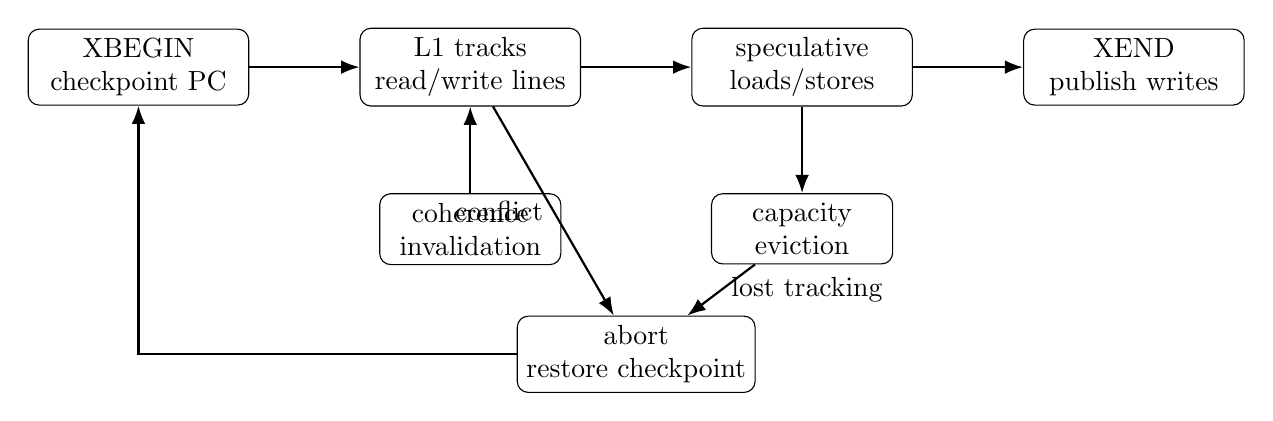
\begin{tikzpicture}[
    box/.style={draw, rounded corners, align=center, minimum width=2.8cm, minimum height=0.9cm},
    smallbox/.style={draw, rounded corners, align=center, minimum width=2.3cm, minimum height=0.8cm},
    arr/.style={-{Latex}, thick}
]
\node[box] (begin) {XBEGIN\\checkpoint PC};
\node[box, right=1.4cm of begin] (track) {L1 tracks\\read/write lines};
\node[box, right=1.4cm of track] (body) {speculative\\loads/stores};
\node[box, right=1.4cm of body] (commit) {XEND\\publish writes};

\node[smallbox, below=1.1cm of track] (inv) {coherence\\invalidation};
\node[smallbox, below=1.1cm of body] (evict) {capacity\\eviction};
\node[box, below=1.1cm of $(inv)!0.5!(evict)$] (abort) {abort\\restore checkpoint};

\draw[arr] (begin) -- (track);
\draw[arr] (track) -- (body);
\draw[arr] (body) -- (commit);
\draw[arr] (inv) -- (track);
\draw[arr] (track) -- node[left, align=center]{conflict} (abort);
\draw[arr] (evict) -- node[right, align=center]{lost tracking} (abort);
\draw[arr] (body) -- (evict);
\draw[arr] (abort.west) -| (begin.south);
\end{tikzpicture}
\caption{Coherence-based HTM treats invalidations and capacity loss as abort signals. Commit is cheap only while the read and write sets remain tracked in cache.}
\label{fig:htm-coherence-abort}
\end{figure}

\section{Modern HTM Implementations}
\begin{itemize}
    \item Intel RTM (xbegin/xend/xabort) – best‑effort contract.
    \item ARM TME – similar concepts, different implementation details.
    \item Capacity and instruction‑based abort causes.
    \item IBM implementations (Blue Gene/Q, POWER8/9) as the longevity case study of coherence-based HTM.
    \item The `best-effort' contract: no guarantee of commit; software must provide a fallback path on abort.
    \item Fallback design: from serialized retry to hybrid HTM+STM (phased hybrid, HSTM), and the glibc lock-elision lesson (elision removed in glibc 2.35).
    \item Abort causes beyond conflicts: capacity, `unsupported instruction', page faults, and how profiling attributes them (Part~VII).
\end{itemize}

\begin{table}[htbp]
\centering
\begin{tabular}{p{0.18\textwidth}p{0.25\textwidth}p{0.25\textwidth}p{0.22\textwidth}}
\hline
\textbf{Mechanism} & \textbf{Tracking} & \textbf{Abort sources} & \textbf{Software obligation}\\
\hline
Intel RTM & Cache-resident speculative read/write sets; explicit \texttt{\_xbegin}, \texttt{\_xend}, \texttt{\_xabort}. & Conflict, capacity, unsupported instruction, interrupt, page fault, explicit abort. & Always provide a correct fallback; subscribe to fallback lock inside the transaction.\\
ARM TME & Architectural transaction begin/end with implementation-defined tracking. & Similar best-effort causes; exact diagnostics are implementation-specific. & Same best-effort rule; never assume eventual commit.\\
IBM POWER HTM & Coherence-based tracking with a mature architectural interface. & Conflict, capacity, non-transactional events, implementation limits. & Use retry budgets and fallback paths; exploit richer platform diagnostics where available.\\
gem5 Ruby/TME model & Simulated cache hierarchy and coherence protocol. & Observable conflict and capacity behavior under controlled cache parameters. & Use simulation to separate effects that hardware counters collapse.\\
\hline
\end{tabular}
\caption{HTM implementations differ in interface and diagnostics, but share the same semantic contract: hardware commit is opportunistic and software fallback is mandatory.}
\label{tab:htm-implementations}
\end{table}

\section{Worked Example: RTM, From the Inside}
\index{HTM}\index{RTM}\index{xbegin}\index{xend}
\label{sec:rtm-example}

Intel RTM is the closest commodity hardware comes to a transaction:

\begin{lstlisting}[language=C, caption={The RTM contract: begin, body, fall back on abort.}]
unsigned status = _xbegin();
if (status == _XBEGIN_STARTED) {
    /* transactional region */
    *a -= n; *b += n;            /* both become visible atomically */
    _xend();                     /* commit                        */
} else {
    /* abort: status encodes the reason (conflict, capacity, ...) */
    lock(&g_fallback);           /* best-effort -> serial fallback  */
    *a -= n; *b += n;
    unlock(&g_fallback);
}
\end{lstlisting}

\begin{itemize}
    \item Compare with \S\ref{sec:api-example}: the STM retry loop becomes a hardware fallback instead of a software retry.
    \item The \texttt{status} byte is the entire diagnostics interface --- the abort-accounting of Part~VI is far richer, which is why profiling tools must infer RTM reasons (Part~VII).
    \item Exercise~1 asks for the fallback design; the phased-hybrid and HSTM bullets above are exactly this fallback made adaptive.
    \item The transaction's atomicity is enforced by the L1/L2 coherence tracking of the first section --- which is why capacity aborts are unavoidable (see Part~VII's GPU contrast).
    \item \textbf{Abort taxonomy}: RTM collapses many causes into one status byte. The practical breakdown is: \emph{conflict} (another core touched the read/write set), \emph{capacity} (the transaction outgrew the L1 tracking --- unavoidable at large read/write sets), \emph{unsupported instruction} (e.g.\ most syscalls and \texttt{rdfsbase}), and \emph{debug/explicit} (\texttt{\_xabort} or debugger single-step). Profilers cannot distinguish conflict from capacity reliably from the status alone --- the reason the Part~VII simulator model re-measures them.
    \item \textbf{Fallback correctness is the real contract.} The \texttt{lock(\&g\_fallback)} path above is a second, serial execution of the same body. It must be \emph{called with the same state view} as the aborted TSX attempt and must itself be transactional-safe: a crash between the fallback lock and its unlock is indistinguishable from a crash inside the transaction. The failure mode to design against is the \emph{retry loop deadlock}: a hybrid that falls back to a lock but is also invoked by the STM-style retry loop can deadlock on its own fallback mutex (a real bug class in the companion repo's SPHT backend).
\end{itemize}

\section{Worked Example: RTM Bank Transfer with Lock Subscription}
\index{lock subscription}\index{fallback lock}\index{money conservation}
\label{sec:rtm-bank-transfer}

The fallback lock must be visible to the hardware transaction. Otherwise a serialized fallback transfer can race with a hardware transaction that never read the lock.

\begin{lstlisting}[language=C, caption={A compilable RTM bank transfer with account floors and fallback lock subscription.}]
/* Compile on x86-64 with:
 *   c++ -std=c++17 -O2 -mrtm bank_rtm.cc -o bank_rtm
 */
#include <immintrin.h>
#include <atomic>
#include <array>
#include <cassert>
#include <thread>

struct Account {
    long balance;
    long floor;
};

static std::atomic<bool> g_fallback{false};

static void lock_fallback() {
    bool expected = false;
    while (!g_fallback.compare_exchange_weak(
               expected, true,
               std::memory_order_acquire,
               std::memory_order_relaxed)) {
        expected = false;
        std::this_thread::yield();
    }
}

static void unlock_fallback() {
    g_fallback.store(false, std::memory_order_release);
}

static bool transfer_body(Account& from, Account& to, long amount) {
    if (amount < 0) return false;

    __int128 after = static_cast<__int128>(from.balance) - amount;
    if (after < from.floor) return false;

    from.balance -= amount;
    to.balance += amount;
    return true;
}

static bool transfer(Account& from, Account& to, long amount) {
    for (int attempt = 0; attempt < 8; ++attempt) {
        unsigned status = _xbegin();

        if (status == _XBEGIN_STARTED) {
            /*
             * Lock subscription: if the fallback path is active, abort.
             * The load places g_fallback in the transactional read set.
             */
            if (g_fallback.load(std::memory_order_acquire))
                _xabort(0xF0);

            bool ok = transfer_body(from, to, amount);
            _xend();
            return ok;
        }

        if ((status & _XABORT_EXPLICIT) &&
            _XABORT_CODE(status) == 0xF0) {
            std::this_thread::yield();
            continue;
        }

        if ((status & _XABORT_RETRY) == 0)
            break;
    }

    lock_fallback();
    bool ok = transfer_body(from, to, amount);
    unlock_fallback();
    return ok;
}

static long total(const std::array<Account, 2>& a) {
    return a[0].balance + a[1].balance;
}

int main() {
    std::array<Account, 2> bank = {{{100, 0}, {100, 0}}};

    long before = total(bank);
    bool ok1 = transfer(bank[0], bank[1], 25);
    bool ok2 = transfer(bank[0], bank[1], 1000);

    assert(ok1);
    assert(!ok2);
    assert(bank[0].balance >= bank[0].floor);
    assert(bank[1].balance >= bank[1].floor);
    assert(total(bank) == before);
}
\end{lstlisting}

\begin{itemize}
    \item The invariant is money conservation: every successful transfer subtracts and adds the same amount.
    \item The account-floor check is inside both the RTM path and the fallback path; fallback is not a different algorithm.
    \item The transaction reads \texttt{g\_fallback}. That read is not an optimization; it is the synchronization point between hardware and software execution.
    \item The retry budget is deliberately finite. A best-effort HTM transaction is allowed to abort forever.
    \item The explicit abort code \texttt{0xF0} separates ``fallback lock is held'' from ordinary conflicts in local diagnostics. It does not make RTM deterministic.
\end{itemize}

\section{Simulation with gem5}
\begin{itemize}
    \item Gem5's Ruby memory system and HTM support for ARM TME.
    \item Running a minimal HTM workload and measuring abort rates.
    \item Why simulation is the only way to study transient effects (evictions mid-transaction, coalescing, contention within a coherence domain).
    \item The workflow: model the cache hierarchy, enable TME, inject a workload, and separate conflict aborts from capacity aborts in output.
\end{itemize}

\section{Worked Example: Model Checking HTM Abort and Fallback}
\index{TLA+}\index{abort}\index{fallback path}
\label{sec:htm-fallback-tla}

A small model is enough to expose the essential rule: abort may occur at any time before commit, and fallback must preserve the same invariants as the hardware path.

\begin{lstlisting}[language={}, caption={TLA+ model of one transferring transaction, abort, interference, and fallback.}]
-------------------------- MODULE BankHTMFallback --------------------------
EXTENDS Integers, TLC

Accounts == {0, 1}
InitA == 100
InitB == 100
Floor == 0
Amt == 7

VARIABLES bal, pc, snap

vars == <<bal, pc, snap>>

Total(b) == b[0] + b[1]

CanMove(b) == b[0] - Amt >= Floor

Move(b) == [b EXCEPT ![0] = @ - Amt,
                      ![1] = @ + Amt]

Init ==
    /\ bal = [a \in Accounts |-> IF a = 0 THEN InitA ELSE InitB]
    /\ pc = "idle"
    /\ snap = bal

Begin ==
    /\ pc = "idle"
    /\ pc' = "tx"
    /\ snap' = bal
    /\ UNCHANGED bal

Abort ==
    /\ pc = "tx"
    /\ pc' = "idle"
    /\ UNCHANGED <<bal, snap>>

Commit ==
    /\ pc = "tx"
    /\ bal = snap
    /\ CanMove(snap)
    /\ bal' = Move(bal)
    /\ pc' = "idle"
    /\ snap' = snap

CommitNoFunds ==
    /\ pc = "tx"
    /\ bal = snap
    /\ ~CanMove(snap)
    /\ pc' = "idle"
    /\ UNCHANGED <<bal, snap>>

Fallback ==
    /\ pc = "idle"
    /\ CanMove(bal)
    /\ bal' = Move(bal)
    /\ pc' = "idle"
    /\ UNCHANGED snap

InterfereAbort ==
    /\ pc = "tx"
    /\ CanMove(bal)
    /\ bal' = Move(bal)
    /\ pc' = "idle"
    /\ snap' = snap

Next ==
    \/ Begin
    \/ Abort
    \/ Commit
    \/ CommitNoFunds
    \/ Fallback
    \/ InterfereAbort

Spec == Init /\ [][Next]_vars

MoneyConserved == Total(bal) = InitA + InitB

FloorSafe == \A a \in Accounts : bal[a] >= Floor

THEOREM Spec => []MoneyConserved
THEOREM Spec => []FloorSafe
=============================================================================
\end{lstlisting}

\begin{itemize}
    \item \texttt{Commit} requires \texttt{bal = snap}. This is the abstract coherence check: if the snapshot is stale, hardware must not commit it.
    \item \texttt{InterfereAbort} models another successful transfer that conflicts with the running transaction. The running transaction aborts, but money is still conserved.
    \item \texttt{Fallback} executes only from \texttt{idle}; it is serialized with respect to the modeled hardware transaction.
    \item Both invariants are safety properties. They do not claim that a best-effort transaction eventually commits.
\end{itemize}

\section{Summary}
\begin{itemize}
    \item HTM leverages existing hardware speculation to implement transactions with near‑zero software overhead.
    \item Limited capacity and unpredictable aborts remain the main challenges.
\end{itemize}

\section{Exercises}
\begin{enumerate}
    \item In Intel RTM, a transaction that exceeds the L1 cache capacity always aborts. Propose a software fallback path and discuss its performance implications.
    \item Using a conceptual pipeline diagram, show why a transaction that triggers a TLB miss is likely to abort.
    \item Configure gem5 to run a simple transactional program and measure the abort rate as the number of cache lines touched increases. Explain the trend.
    \item \emph{[implementation]} Extend Listing~\ref{sec:rtm-bank-transfer}'s transfer code to collect per-thread counters for commits, explicit fallback-lock aborts, retryable aborts, and non-retryable aborts. Keep the counters outside the transaction and explain why updating them inside RTM would distort the measured abort rate.
    \item \emph{[verification]} Modify the TLA+ model in \S\ref{sec:htm-fallback-tla} so that transfers may go in both directions. State and check the money-conservation invariant and an account-floor invariant for both accounts.
    \item \emph{[theory]} Explain why lock subscription is necessary for opacity in a hybrid HTM plus lock fallback design. Give an execution in which omitting the subscription lets a hardware transaction commit concurrently with the fallback critical section.
\end{enumerate}

\chapter{Transactional Memory for GPUs}
\label{chap:gpu-tm}

Every chapter so far has leaned on two structural facts about commodity
processors: a cache-coherence protocol that can be exploited for conflict
detection, and speculative hardware that can roll a thread back on an abort.
GPUs provide neither. This chapter explains why the whole CPU-centred design
space of Parts~II, IV, and VII must be rebuilt, and how a distinct GPU TM
design space has emerged in its place: lock-step warp execution, software
conflict detection, multi-versioned commit logs, and batch commit.

\section{The GPU Execution Model}

A modern GPU is a throughput-oriented device. It does not try to make one
thread fast; it runs tens of thousands of threads and hides memory latency
by switching between them. The execution model that results is SIMT
(single instruction, multiple threads):

\begin{itemize}
    \item \textbf{Warps and lock step.} 32 threads (a warp; AMD calls it a
          wavefront of 64) share a single program counter. One instruction is
          broadcast to all lanes of a warp each cycle. Lanes that should not
          take a path are masked off rather than branched around
          (divergence, Section~\ref{sec:ballot}).
    \item \textbf{Free-for-all scheduling.} The hardware interleaves warps on
          a streaming multiprocessor (SM) to hide latency. There is no
          fairness contract and no guarantee that a warped-out thread makes
          progress.
    \item \textbf{Threads are pinned.} A thread occupies its lane for the
          lifetime of the kernel. There is no thread migration and, crucially,
          no analogue of the CPU \texttt{sigsetjmp}/\texttt{siglongjmp}
          rollback that CPU STMs use to restart aborted transactions.
    \item \textbf{A weak memory model.} Global memory is relaxed. Ordering is
          restored only by explicit device-scope fences
          (\texttt{\_\_threadfence()}) or block/system-scope variants.
\end{itemize}

\textbf{The decisive absence is cache coherence.} GPU L1 caches are private
to an SM and are not kept coherent. Threads in different SMs synchronise only
through the L2 cache and global memory, by explicit atomic operations
(\texttt{atomicAdd}, \texttt{atomicCAS}, \texttt{atomicInc},
\texttt{atomicExch}). Hardware transactional memory in the sense of Herlihy
and Moss --- transactional states layered onto a snooping coherence protocol
\cite{herlihy93} --- has no substrate on which to be built. Everything that
Parts~II and VII established about coherence-based conflict detection and
speculative stores simply does not apply.

\section{Three Foundational Absences}

\begin{itemize}
    \item \textbf{No hardware TM on the market.} Neither NVIDIA nor AMD
          exposes transactional instructions to programmers. Every published
          GPU HTM design --- KILO~TM, WarpTM, the snapshot-isolation HTM ---
          exists only in simulation
          \cite{fung11kilotm,fung13warptm,chen17snapshot}. GPU TM on real
          silicon is software TM.
    \item \textbf{No speculative state.} There is no reorder buffer, store
          buffer, or speculation queue whose flush undoes a transaction. An
          abort is a software action: discard the write-set, reset
          transaction-local state, and re-execute the body.
    \item \textbf{One coherent point, shared.} The only memory level at which
          threads can observe each other is L2. Metadata such as lock tables,
          versioned boxes, and commit logs must live there --- and every probe
          of that metadata competes for the same atomics bandwidth as the
          program's data. Eager (visible) reads, which a CPU STM hides behind
          its L1, are prohibitively expensive at GPU scale.
\end{itemize}

The consequence: the GPU TM design space is \emph{exactly} the software-TM
space of Part~IV, but solved under constraints the CPU never imposes. The
rest of this chapter is about those constraints.

\section{Lock-Step Execution, Divergence, and the Ballot Contract}
\label{sec:ballot}

A warp executes one instruction for all its lanes at once. Computation on
lane-local values is SIMD-cheap; computation that depends on \emph{which}
lanes are active --- voting, reduction, convergence --- is different: it must
be performed collectively by every active lane at the same instruction.

\textbf{You cannot spin.} If a lane spins on a lock held by another lane of
the same warp, the whole warp stalls --- owner included --- and deadlocks.
CPU-style spin-based contention management (TL2's commit lock, TinySTM's
spin) \cite{dice06tl2,riegel06disc} is therefore unusable. GPU STMs replace
waiting with \emph{self-abort}: lock sorting (GPU-STM
\cite{xu14gpustm}), priority-based lock stealing (PR-STM
\cite{shen15prstm}), or warp-mask retry (the lightweight STMs of Holey and
Zhai \cite{holey14}).

\textbf{Conflict detection becomes a warp vote.} Because lock step is cheap,
the whole warp can resolve its intra-warp conflicts in one transaction using
\texttt{\_\_ballot\_sync}, the primitive that collects one predicate bit from
each lane into a 32-bit mask. Predicate voting replaces the point-to-point
messages of a CPU coherence protocol.

But the ballot carries a contract that is easy to violate:
\textbf{every active lane must reach the call}. Guarding a ballot behind a
per-lane condition is undefined behaviour that silently misbehaves on some
NVIDIA silicon and raises a fatal HSA exception on AMD ROCm. The portable
pattern hoists the ballot out of the lane-guarded block and lets lane~0 act
on the result:

\medskip
\noindent\textbf{Scope of ``lock step.''} ``Lock-step'' here means the
\textit{architectural} contract of a warp in the SM's current scheduling
model, not a hardware guarantee of perfect temporal lock-step. On NVIDIA,
the independent thread scheduler (Volta and later) permits lanes of one
warp to diverge in \emph{execution} while preserving converged semantics
only at explicit reconvergence points (\texttt{\_\_syncwarp}, ballots).
AMD's wavefront semantics differ again (two quads, predication-based
execution). Every assumption this chapter makes about ballot-based
coordination --- all active lanes at the call, uniform trip counts in
loops feeding a ballot --- therefore holds \emph{as a programming
contract we adopt}, verified on the backends by on-target tests and the
formal models of Section~\ref{sec:tla}, rather than as a fact of the
hardware.

\begin{verbatim}
/* BROKEN: the ballot executes only when lane == 0 (undefined). */
if (lane == 0) {
    uint64_t m = __ballot_sync(~0ULL, conflict);
    if (m) flag = 1;
}

/* CORRECT: every lane executes the ballot; lane 0 acts on it. */
{
    uint64_t m = __ballot_sync(~0ULL, conflict);
    if (lane == 0 && m) flag = 1;
}
\end{verbatim}

The same contract applies to \texttt{\_\_syncwarp()} and to any loop that
feeds a ballot: a short-circuited loop such as
\texttt{for (w = 0; w < n \&\& !conflict; ++w)} lets some lanes exit early
and desynchronises the barrier inside the loop body. These are not exotic
theoretical failures; both were real bugs found while porting the GPU
backends of this book to AMD hardware, and both were caught only by
on-target testing and by the formal models of Section~\ref{sec:tla}. The
lesson is uniform: \textbf{every lane must enter every synchronous
primitive}.

\section{Worked Example: Counting Aborts With a Ballot}
\index{warp}\index{\_\_ballot\_sync}\index{GPU TM}\index{SIMT}\index{wavefront}\index{divergence}\index{private memory}\index{versioned box}\index{multi-version TM}
\label{sec:ballot-example}

Predicate voting turns an abort decision into a warp-wide count. PR-STM and
the GUST-style backends use this exact pattern to let a warp resolve
intra-warp conflicts in one instruction:

\begin{lstlisting}[language=C++, caption={Counting aborted lanes with \_\_ballot\_sync.}]
bool conflict = (read_set_overlap(&mine, &yours, lane));
/* every lane executes the ballot -- never inside `if (lane == k)` */
uint32_t mask = __ballot_sync(0xffffffffu, conflict);
if (lane == 0) {
    int aborted = __popc(mask);      /* lanes that lost the vote */
    if (aborted == WARP_SIZE) { /* deadlock-free: nobody can proceed */ }
}
\end{lstlisting}

\begin{itemize}
    \item The 32-bit \texttt{mask} is one bit per lane; \texttt{\_\_popc}
          counts the losers in a single instruction.
    \item This is the software replacement for the coherence messages a CPU
          protocol would send: one vote replaces 32 point-to-point
          invalidation checks.
    \item Exercise~4 of this chapter asks exactly for this pattern; the
          TLA+ models of Section~\ref{sec:tla} represent the same count as an
          \texttt{activeMask} update.
\end{itemize}

\section{Capacity: Large Read/Write Sets in a Shallow Memory Hierarchy}
\label{sec:capacity}

A CPU transaction's read-set and write-set grow in registers and L1,
decoupled from the machine's storage capacity by fast private caches. A GPU
thread has almost nothing:

\begin{itemize}
    \item The \textbf{register file} is the only per-thread storage, a few
          words per lane. A read-set of even a few hundred entries cannot
          live there.
    \item Per-thread \emph{local memory} is really a private slice of global
          memory: cached in L1 when it fits, spilled to L2 when it does not.
          Every spill costs bandwidth and latency.
    \item \emph{Shared memory} (tens of KB per block) is the natural home of
          a warp's transaction descriptor and read/write set, but its size
          --- and the fact that it is shared among a block's threads --- makes
          it a scarce, contended resource. Large transactions spill their sets
          to global memory.
    \item The natural conflict-detection granularity is the 32-bit word or
          the 128-byte cache line, not the object. Irregular workloads such as
          the STAMP kernels (\texttt{bayes}, \texttt{intruder},
          \texttt{labyrinth}) \cite{minh08stamp} routinely touch hundreds of
          distinct lines per transaction.
\end{itemize}

\textbf{Compaction is mandatory.} Hardware designs use Bloom-filter read-set
signatures (KILO TM \cite{fung11kilotm}); software designs compact the
read-set to version metadata or use per-address lock tables
\cite{shen15prstm,nunes22csmv}. The engineering rule of thumb is simple: a
transaction whose tracked footprint does not fit on chip is a capacity abort
waiting to happen --- and on a GPU, \emph{every} transaction competes with
every other transaction in the same block for the same on-chip space.

\textbf{Coalescing cuts both ways.} When 32 lanes access 32 consecutive
addresses, the hardware merges them into one wide memory transaction --- a
gift to throughput. When a transactional workload accesses \emph{scattered}
addresses (hash tables, trees, linked lists --- the furniture of GPU STM
benchmarks), the memory subsystem instead serialises 32 narrow accesses, one
per lane, and coalescing stops helping. The access pattern of the workload,
not the TM algorithm, often dominates measured performance.

\section{Worked Example: Warp-Uniform Bank Transfer With Self-Abort}
\label{sec:gpu-bank-transfer-example}
\index{bank transfer}\index{self-abort}\index{warp}\index{money conservation}\index{account floor}

The bank benchmark is a useful minimal GPU TM workload: each transaction reads
two balances, checks the source account floor, and either transfers a fixed
amount or aborts without changing state. The kernel below is deliberately
small. It is not a full STM; it is the lock-based shape that GPU STMs refine:
acquire metadata without spinning, perform the update only after both locks
are held, and use a warp-uniform ballot to count aborts.

\begin{lstlisting}[language=C++, caption={A CUDA bank-transfer kernel using sorted locks and warp-uniform abort counting.}]
#include <stdint.h>

#ifndef WARP_SIZE
#define WARP_SIZE 32
#endif

__device__ __forceinline__ int lane_id() {
    return threadIdx.x & (WARP_SIZE - 1);
}

__device__ __forceinline__ int lock_account(int *locks, int id) {
    return atomicCAS(&locks[id], 0, 1) == 0;
}

__device__ __forceinline__ void unlock_account(int *locks, int id) {
    __threadfence();          /* publish balance writes before unlocking */
    atomicExch(&locks[id], 0);
}

/* Each lane attempts one transfer:
     from[i] -> to[i], amount[i].
   On success, total money is unchanged. On abort, no balance is changed. */
__global__ void bank_transfer_kernel(int *balances,
                                     const int *floors,
                                     int *locks,
                                     const int *from,
                                     const int *to,
                                     const int *amount,
                                     int n,
                                     unsigned int *abort_count) {
    int tid = blockIdx.x * blockDim.x + threadIdx.x;
    int lane = lane_id();

    bool abort_tx = false;
    bool committed = false;

    if (tid < n) {
        int a = from[tid];
        int b = to[tid];
        int x = amount[tid];

        if (a == b || x < 0) {
            abort_tx = true;
        } else {
            int first  = (a < b) ? a : b;
            int second = (a < b) ? b : a;

            int got_first = lock_account(locks, first);
            int got_second = 0;

            if (got_first) {
                got_second = lock_account(locks, second);
            }

            if (!got_first || !got_second) {
                abort_tx = true;        /* no spin: retry in a later kernel pass */
            } else {
                int ba = balances[a];
                int bb = balances[b];

                if (ba - x < floors[a]) {
                    abort_tx = true;    /* account floor would be violated */
                } else {
                    balances[a] = ba - x;
                    balances[b] = bb + x;
                    committed = true;
                }

                unlock_account(locks, second);
                unlock_account(locks, first);
            }

            if (got_first && !got_second) {
                unlock_account(locks, first);
            }
        }
    }

    /* Every active lane reaches the ballot, including lanes with tid >= n. */
    unsigned int mask = __ballot_sync(0xffffffffu, abort_tx);
    if (lane == 0) {
        atomicAdd(abort_count, (unsigned int)__popc(mask));
    }

    (void)committed;          /* retained for instrumentation builds */
}
\end{lstlisting}

\begin{itemize}
    \item Lock acquisition is sorted by account id, but failure does not spin.
          The transaction self-aborts and can be retried by the enclosing
          driver.
    \item The transfer writes both balances only after both locks are held.
          Therefore a committed transaction preserves the total balance; an
          aborted transaction writes nothing.
    \item The ballot is outside the per-lane transaction body. Even inactive
          lanes execute it with \texttt{abort\_tx == false}, preserving the
          SIMT contract of Section~\ref{sec:ballot}.
    \item The device fence before \texttt{atomicExch} is the publication edge:
          data writes must reach global visibility before another lane can
          acquire the account lock.
\end{itemize}

\begin{figure}[htbp]
\centering
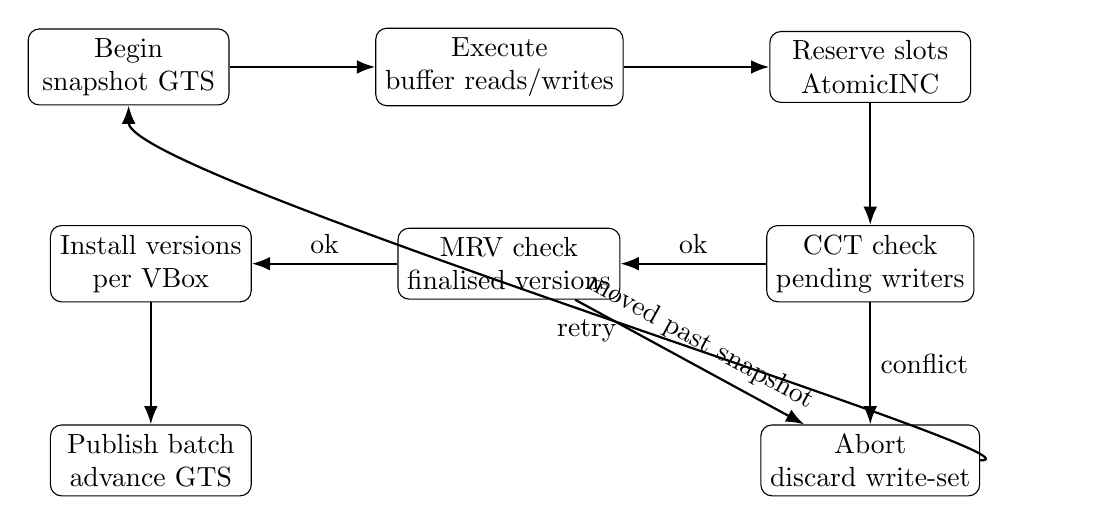
\begin{tikzpicture}[
    node distance=1.55cm and 1.85cm,
    state/.style={draw, rounded corners, align=center, minimum width=2.55cm, minimum height=0.9cm},
    arrow/.style={-Latex, thick}
]
\node[state] (begin) {Begin\\snapshot GTS};
\node[state, right=of begin] (exec) {Execute\\buffer reads/writes};
\node[state, right=of exec] (reserve) {Reserve slots\\AtomicINC};
\node[state, below=of reserve] (cct) {CCT check\\pending writers};
\node[state, left=of cct] (mrv) {MRV check\\finalised versions};
\node[state, left=of mrv] (write) {Install versions\\per VBox};
\node[state, below=of write] (publish) {Publish batch\\advance GTS};
\node[state, below=of cct] (abort) {Abort\\discard write-set};

\draw[arrow] (begin) -- (exec);
\draw[arrow] (exec) -- (reserve);
\draw[arrow] (reserve) -- (cct);
\draw[arrow] (cct) -- node[above, sloped] {ok} (mrv);
\draw[arrow] (mrv) -- node[above, sloped] {ok} (write);
\draw[arrow] (write) -- (publish);

\draw[arrow] (cct) -- node[right] {conflict} (abort);
\draw[arrow] (mrv) -- node[above, sloped] {moved past snapshot} (abort);
\draw[arrow] (abort.east) .. controls ($(abort.east)+(1.1,0)$) and ($(begin.south)+(0,-0.9)$) .. node[below] {retry} (begin.south);
\end{tikzpicture}
\caption{A GUST-style GPU commit path. Slot reservation is non-blocking; validation is split between concurrently committing transactions and already finalised versions.}
\label{fig:gpu-gust-commit-path}
\end{figure}


\section{Commit at GPU Scale: From Serial Locks to Batched Multi-Versioning}
\label{sec:commit}

A CPU system runs a few dozen cores; a GPU kernel launches thousands of
\emph{concurrent transactions}. Every single-threaded choke point of a CPU
TM becomes a hard bottleneck:

\begin{itemize}
    \item \textbf{No commit locks.} A global commit lock that serialises
          commits (as in TL2 \cite{dice06tl2}) or any CAS-based append to a
          shared structure leads to one winner and thousands of spinning
          losers. GUST reports that an AtomicINC-based commit-log append
          sustains roughly \textbf{100$\times$ more concurrent commits} than
          a CAS-based append at RTX~6000 scale \cite{nunes23gust}. The design
          rule: commit-slot allocation must be \emph{never-failing}
          (AtomicINC), not \emph{contended} (CAS).
    \item \textbf{Validation cost is a sum, not a constant.} Commit-time
          validation is $O(|\text{read-set}|)$ per transaction and happens for
          thousands of transactions per batch, so the aggregate is
          $O(\sum |\text{read-set}|)$; validation against \emph{concurrently
          committing} transactions adds a cross-product term. Cheap
          per-transaction costs explode multiplicatively at GPU concurrency.
    \item \textbf{Multi-versioning kills the abort chain.} If a transaction
          reads a consistent old snapshot instead of watching for conflicts,
          read-only transactions \emph{never abort}. This property, inherited
          from JVSTM \cite{cachopo06}, is what makes the most scalable GPU
          STMs (CSMV \cite{nunes22csmv}, GUST \cite{nunes23gust})
          multi-versioned: writers append versions and readers walk history,
          instead of every read being a potential conflict.
    \item \textbf{Batch everything.} Because warps move in lock step, the
          natural unit of commit is \emph{the warp}, not the thread. GUST has
          a warp reserve \texttt{WARP\_SIZE} contiguous commit-log slots with
          one AtomicINC, validate as a group, write back, and publish the
          batch with a single advance of the global timestamp
          \cite{nunes23gust}. CSMV goes further and decouples execution from
          commit entirely, dedicating \emph{server warps} to validate and
          commit the writes of \emph{client warps} \cite{nunes22csmv}.
\end{itemize}

\section{Worked Example: Commit-Slot Allocation, CAS vs.\ AtomicINC}
\index{AtomicINC}\index{commit log}\index{commit-slot allocation}\index{CCT}\index{MRV}\index{GTS}\index{versioned box}\index{batch publication}\index{GPU TM}
\label{sec:slot-example}

The ``never-failing not contended'' rule of the previous section, in code.
Two ways for a warp to claim commit-log slots:

\begin{lstlisting}[language=C++, caption={CAS vs.\ AtomicINC commit-slot reservation.}]
/* CAS: one winner per contention point; losers spin or retry. */
while (!atomicCAS(&g_next, base, base + WARP_SIZE)) {}  /* convoy */

/* AtomicINC: never fails; every warp claims its own slots. */
int base = atomicAdd(&g_next, WARP_SIZE);   /* no retry, no loop */
\end{lstlisting}

\begin{itemize}
    \item Both allocate \texttt{WARP\_SIZE} contiguous slots; the CAS version
          makes concurrent warps contend for the \emph{right} to allocate,
          the AtomicINC version lets them all allocate and sort it out later.
    \item GUST reports this single choice sustains roughly $100\times$ more
          concurrent commits than a CAS append at RTX~6000 scale
          \cite{nunes23gust} --- the ``no commit locks'' bullet quantified.
    \item The \texttt{base} value is the warp's commit timestamp; lane
          \texttt{l} owns slot \texttt{base + l}, exactly the GUST batch
          publication of Section~\ref{sec:gust}.
    \item The TLA+ model of Section~\ref{sec:tla} abstracts the AtomicINC as
          one atomic action per warp --- the whole batch in one step.
\end{itemize}

\begin{table}[htbp]
\centering
\begin{tabular}{p{0.14\linewidth}p{0.15\linewidth}p{0.13\linewidth}p{0.16\linewidth}p{0.26\linewidth}}
\hline
\textbf{Commit style} & \textbf{Allocator} & \textbf{Waiting} & \textbf{Reader rule} & \textbf{GPU consequence} \\
\hline
Global lock & one lock & spin or block & single latest value &
Simple, but one serial point throttles thousands of lanes. \\
CAS log append & CAS on tail & retry loop & latest or validated value &
Correct but creates a convoy when many warps append together. \\
AtomicINC log append & atomic add on tail & none for allocation & snapshot plus validation &
Every warp obtains slots; conflicts are handled by validation, not allocation failure. \\
Client--server commit & server warp queue & client waits for service & multi-version snapshot &
Moves contended metadata to server warps; best suited when commit work can be amortised. \\
Read-only MVCC & none on read path & none & stable old version &
Read-only transactions never abort, matching the JVSTM and CSMV design point. \\
\hline
\end{tabular}
\caption{GPU commit strategies differ mainly in where they place the serialisation point.}
\label{tab:gpu-commit-strategies}
\end{table}


\section{A Taxonomy of GPU TM}
\label{sec:taxonomy}

Table~\ref{tab:gpu-tm} summarises the main published designs, both the
simulated hardware proposals and the software systems that run on real
silicon. All of the software rows are realised, at some level, in the
backends accompanying this book: PR-STM in
\texttt{backends\slash{}tm\_impl\slash{}gpu\_stm}, CSMV in \texttt{backends\slash{}tm\_impl\slash{}csmv},
GPUTX in \texttt{backends\slash{}tm\_impl\slash{}gputx}, and GUST in
\texttt{gpu\slash{}backends\slash{}gpu\_gust}.

\begin{table}[ht]
\centering
\begin{tabular}{lllp{9cm}}
\hline
\textbf{System} & \textbf{Year} & \textbf{Type} & \textbf{Key idea} \\
\hline
KILO TM \cite{fung11kilotm} & 2011 & HW & word-level, value-based conflicts; commit units; no coherence \\
WarpTM \cite{fung13warptm} & 2013 & HW & warp-level management; temporal conflict detection \\
SI-HTM \cite{chen17snapshot} & 2017 & HW & multi-version memory; snapshot isolation; write-skew elimination \\
GPU-STM \cite{xu14gpustm} & 2014 & SW & encounter-time lock sorting to avoid deadlock \\
Lightweight \cite{holey14} & 2014 & SW & eager/pessimistic/invisible reads; warp-mask retry \\
PR-STM \cite{shen15prstm} & 2015 & SW & 32-bit priority lock word; lock stealing; commit-time validation \\
CSMV \cite{nunes22csmv} & 2022 & SW & multi-version; client--server commit (server warps validate) \\
OFG-STM \cite{perlin24ofg} & 2024 & SW & obstruction-free; locator ownership; warp GC \\
GUST \cite{nunes23gust} & 2023 & SW & AtomicINC commit log; CCT/MRV validation; batch publication \\
\hline
\end{tabular}
\caption{A taxonomy of GPU TM systems.}
\label{tab:gpu-tm}
\end{table}

\section{Hardware Proposals: KILO TM, WarpTM, and Snapshot Isolation}
\label{sec:hardware}

The hardware line of work, all simulation-based, shows what a future GPU
vendor could ship. KILO~TM \cite{fung11kilotm} was the first credible design:
because GPUs lack coherence, it detects conflicts \emph{by value}, keeping a
read-log and write-log in each thread's local memory and validating them
against committed values at commit units distributed near the L2 banks, using
Bloom filters for compact speculative validation. Its reported $59\%$ of
fine-grained-lock performance on irregular kernels, for an area cost of about
$0.5\%$ of a commercial GPU, is the canonical data point that GPU HTM is
possible but not free.

WarpTM \cite{fung13warptm} added two optimisations to KILO~TM that directly
echo the software concerns of this chapter. \emph{Warp-level transaction
management} resolves intra-warp conflicts before the warp ever reaches the
commit units --- exactly what software warps do with
\texttt{\_\_ballot\_sync} --- so a conflict-free warp commits as a unit and
amortises commit-message traffic. \emph{Temporal conflict detection} lets
read-only transactions commit silently using globally synchronised timers,
attacking the same read-abort problem that multi-versioning attacks in
software. Together they bought roughly $65\%$ throughput and $34\%$ energy
savings over the base design.

The snapshot-isolation HTM \cite{chen17snapshot} extended a multi-versioned
memory system to let write--read conflicts pass, aborting only on
write--write conflicts, and eliminating the associated write-skew anomaly on
the fly. Its motivation --- long transactions over complex data structures
should not die because of reads --- is the same one that drives the MVCC
software systems below.

\section{Software TM in the Wild}
\label{sec:software}

The software systems are what actually runs, and their progression is a
textbook version of the CPU STM evolution of Part~IV:

\begin{itemize}
    \item \textbf{Lock-based.} GPU-STM \cite{xu14gpustm} applies
          encounter-time lock sorting so that a warp never spins on a lock in
          a deadlock-prone lock order. PR-STM \cite{shen15prstm} packs
          \texttt{[priority:8 | version:23 | locked:1]} into a 32-bit lock
          word, acquires locks by priority-aware CAS at commit time, and lets
          a higher-priority transaction \emph{steal} a lock from a
          lower-priority holder, turning contention into a clean self-abort
          instead of a spin. The lightweight STMs of Holey and Zhai
          \cite{holey14} provide three flavours --- eager read-write
          conflicts (ESTM), pessimistic (PSTM), and invisible reads (ISTM)
          --- with shadow metadata in global memory and per-thread logs in
          local memory.
    \item \textbf{Multi-versioned.} CSMV \cite{nunes22csmv} is JVSTM's
          multi-version design \cite{cachopo06} rebuilt for GPU economics:
          \emph{client} warps execute transactions and buffer writes; a few
          \emph{server} warps hold the versioned metadata, validate, and
          commit, so the contended shared state never leaves on-chip storage.
          Read-only transactions never abort.
    \item \textbf{Obstruction-free.} OFG-STM \cite{perlin24ofg} uses
          locator-based ownership and warp-wide garbage collection with
          Cooperative Groups, avoiding locks. Its stated advantage --- a
          warp-cooperative solution to locator reclamation (the GPU analogue
          of hazard pointers) --- is a GPU-native answer to a lock-free
          pain point.
\end{itemize}

\section{Case Study: GUST and the Snapshot Threshold}
\label{sec:gust}

GUST \cite{nunes23gust}, implemented in this project's
\texttt{gpu/backends/gpu\_gust}, is a multi-version system whose one idea is
to replace contended commit-time synchronisation with an AtomicINC. Several
of its design points are worth teaching on their own. It is \emph{one
design point} in the GPU commit-protocol space, not the canonical answer:
the rest of the chapter positions it against serial-lock, per-block-log,
and global-log alternatives (Section ``Commit at GPU Scale''). Several of
its design points are worth teaching on their own:

\begin{itemize}
    \item \textbf{Versioned boxes.} Each address owns a circular buffer of the
          most recent committed \texttt{(timestamp, value)} pairs, appended
          to increasingly (slot = \texttt{head \% DEPTH}).
    \item \textbf{Commit log and GTS.} A bounded global commit log holds the
          state (free, pending, committed, aborted) and write-set of every
          in-flight transaction. A global timestamp (GTS) counts
          \emph{finalised} slots. A transaction snapshots GTS at begin and
          never re-reads earlier than that snapshot.
    \item \textbf{CCT + MRV validation.} On commit a warp validates against
          two classes of earlier transactions: those still finalising
          (compared directly against their commit-log write-sets ---
          concurrently-committing-transaction checking, CCT) and those already
          finalised (checked via the most recent version, MRV --- if any read
          VBox has moved past the snapshot, abort).
    \item \textbf{Batch publication.} A warp reserves \texttt{WARP\_SIZE}
          slots with one AtomicINC, writes back all its versions, and advances
          GTS by \texttt{WARP\_SIZE} only when it observes GTS equal to its
          base --- a full-warp group commit.
\end{itemize}

The subtlety that bit during bring-up illustrates why this chapter exists. An
early kernel draft used \texttt{snapshot = startTS + 1} on the intuition that
a committing transaction becomes visible one tick later. But GTS counts
\emph{finalised} slots: a writer that reserved slot $c$ publishes version
$c+1$ and is visible \emph{iff} $c < startTS$. The naive $+1$ let an
in-flight writer at exactly $c = startTS$ slip into the snapshot --- a
missed-conflict hole that neither validation phase could see. In a CPU STM
paper this would be a footnote; on a GPU, with thousands of concurrent
transactions, it is a data-corruption bug that is only tractable with the
right tools.

\section{Worked Example: The Snapshot Threshold, in Code}
\index{snapshot threshold}\index{CCT}\index{MRV}
\label{sec:snapshot-example}

The off-by-one that Section~\ref{sec:gust} describes, and its fix:

\begin{lstlisting}[language=C++, caption={GUST snapshot: why startTS+1 is a missed-conflict hole.}]
/* GTS counts FINALISED slots. A writer reserving slot c publishes
   version c+1, visible iff c < startTS. */

int snapshot = *gts;                  /* correct: only finalised slots */
// int snapshot = *gts + 1;           /* bug: lets an in-flight writer
//                                        at c == startTS into the read */

/* Suppose startTS = 5 and an in-flight writer holds slot 5 (not yet
   finalised).  The +1 form reads version 6, but that writer publishes
   version 6 only after finalising --- a value that does not exist yet.
   The reader proceeds on a snapshot that was never real. */
\end{lstlisting}

\begin{itemize}
    \item The correct form reads only finalised slots: a writer visible at
          version $v$ must have reserved $v-1 < startTS$, so the read must
          use \emph{startTS}, not \texttt{startTS+1}.
    \item Neither CCT nor MRV validation can catch this: the reader believes
          it has a valid snapshot and never re-checks the in-flight writer.
    \item This is the exercise of this chapter's Exercise~3, and it is
          exactly what the TLA+ model's \texttt{InvNoMissedConflict}
          invariant caught before the kernel was fixed.
\end{itemize}

\section{Worked Example: Money Conservation in TLA+}
\label{sec:gpu-bank-tla-example}
\index{TLA+}\index{model checking}\index{money conservation}\index{account floor}

The following finite TLA+ model captures the semantic contract of the bank
transaction independently of any particular GPU implementation. TLC can check
it directly: each step chooses a source, destination, and amount; a step is
enabled only when the source account remains above its floor. The invariants
are the two properties the GPU kernel must preserve.

\begin{lstlisting}[caption={A finite TLA+ bank-transfer model for TLC.}]
----------------------------- MODULE BankTransferGPU -----------------------------
EXTENDS Naturals, TLC

Accounts == {"A", "B", "C"}

InitBalance == [
  "A" |-> 10,
  "B" |-> 10,
  "C" |-> 10
]

Floor == [
  "A" |-> 2,
  "B" |-> 2,
  "C" |-> 2
]

Amounts == 1..3

VARIABLE bal

Total(b) == b["A"] + b["B"] + b["C"]

Init ==
  bal = InitBalance

Transfer(src, dst, amt) ==
  /\ src \in Accounts
  /\ dst \in Accounts
  /\ src # dst
  /\ amt \in Amounts
  /\ bal[src] >= Floor[src] + amt
  /\ bal' =
       [a \in Accounts |->
          IF a = src THEN bal[a] - amt
          ELSE IF a = dst THEN bal[a] + amt
          ELSE bal[a]]

Next ==
  \E src, dst \in Accounts:
    \E amt \in Amounts:
      Transfer(src, dst, amt)

Spec ==
  Init /\ [][Next]_bal

MoneyConserved ==
  Total(bal) = Total(InitBalance)

FloorsPreserved ==
  \A a \in Accounts:
    bal[a] >= Floor[a]

TypeOK ==
  bal \in [Accounts -> Nat]

=============================================================================
\end{lstlisting}

\begin{itemize}
    \item \texttt{MoneyConserved} is the serial meaning of a transfer: debit
          and credit are one atomic effect.
    \item \texttt{FloorsPreserved} is stronger than absence of negative
          balances; the floor is part of the transaction's precondition.
    \item A GPU TM backend can abort, retry, batch, or multi-version the
          transaction, but a committed history must refine this small model.
    \item This model is also a useful negative test: remove the floor guard
          from \texttt{Transfer} and TLC quickly finds a violation of
          \texttt{FloorsPreserved}.
\end{itemize}


\section{Verifying GPU Protocols with TLA+}
\label{sec:tla}

Because GPU protocols replace hardware guarantees with software discipline,
they are prime candidates for the model-checking workflow of Part~III. The
models accompanying this book --- \texttt{GPU\_PR\_STM.tla},
\texttt{GPU\_SIMT.tla}, \texttt{GPU\_JVSTM.tla}, \texttt{GPU\_GUST.tla} ---
make the warp the unit of concurrency and encode the SIMT lock step as a
shared warp \texttt{phase} with per-thread arrays and an \texttt{activeMask}
to express divergence:

\begin{itemize}
    \item \textbf{Warp-as-process.} One TLA+ process per warp manages all of
          its lanes' transactions; a single transition steps the whole warp,
          matching the shared program counter.
    \item \textbf{Divergence as masking.} Lanes that finish early are removed
          from the active mask; the warp continues with the survivors, exactly
          as a real divergence point does.
    \item \textbf{Bounded phases.} Reads, writes, and validation are explicit
          phases (\texttt{L\_read} $\rightarrow$ \texttt{L\_write}
          $\rightarrow$ \texttt{L\_validate}), bounding the state space by
          \texttt{ReadsPerThread} instead of an unbounded \texttt{either}.
    \item \textbf{Opacity is an invariant.} The GUST model's
          \texttt{InvNoMissedConflict} states that no committed transaction
          may be followed by another committed transaction that wrote an
          address the first one read --- serialisable/opaque semantics, not
          just absence of lost updates.
\end{itemize}

TLC has checked tens of millions of states across these models with no
violations: the GUST model ran 1.9M states on the small configuration (0
errors) and over 25M on the large one without violations before timing out.
The models caught real bugs --- the \texttt{startTS} vs.\
\texttt{startTS+1} snapshot hole of Section~\ref{sec:gust} (found first in
the model, then confirmed in the kernel) and, more fundamentally, the
\texttt{\_\_ballot\_sync} divergence class of Section~\ref{sec:ballot}. The
two tools worked as a pair: TLA+ says \emph{what} must be true; the ballot
contract says \emph{how} the hardware will let you express it.

\section{Summary}

\begin{itemize}
    \item GPUs have no cache coherence, no speculative hardware, and no vendor
          TM: GPU TM is software TM, run at a scale and under constraints the
          CPU design space never anticipated.
    \item Lock-step warp execution turns spinning into self-abort and conflict
          detection into predicate voting via \texttt{\_\_ballot\_sync}.
    \item Read/write sets that do not fit on chip, coalescing that works
          against scattered accesses, and thousands of concurrent transactions
          all push designs toward multi-versioning and batch commit.
    \item The recurring winners --- CSMV's client--server commit and GUST's
          AtomicINC commit log --- trade a serial CAS for an increment, and a
          read abort for a consistent snapshot.
    \item Hardware proposals (KILO TM, WarpTM, snapshot-isolation HTM) show the
          design space is real but simulated; the software systems show it is
          live silicon reality.
    \item Formal models at warp granularity are a practical, not academic,
          tool: they caught the very bugs (the ballot contract, the snapshot
          threshold) that the GPU community has repeatedly tripped over.
\end{itemize}

\section{Exercises}
\begin{enumerate}
    \item A warp of 32 lanes runs a transaction that spins on a lock held by
          another lane of the same warp. Explain on which hardware this
          deadlocks and why. How does PR-STM's priority stealing turn the same
          situation into progress?
    \item GPU-STM sorts locks to avoid deadlock while PR-STM steals locks by
          priority. Contrast the two contention policies under (a) uniformly
          random and (b) skewed (hot-spot) access patterns.
    \item GUST uses \texttt{snapshot = startTS}, not \texttt{startTS + 1}.
          Construct a two-transaction history where the $+1$ variant lets an
          in-flight writer's version appear in a reader's snapshot, and
          explain why neither CCT nor MRV catches it.
    \item Using the ballot pattern of Section~\ref{sec:ballot}, compute the
          number of aborted lanes in a warp via \texttt{\_\_popc} on the
          ballot result, and explain why the ballot cannot be moved inside a
          lane-guarded branch.
    \item CSMV dedicates server warps to committing client warps' writes.
          Identify the serialisation point this creates, and propose how a
          workload dominated by read-only transactions could bypass it.
    \item Using the TLA+ workflow of Part~III, sketch an invariant for a
          warp-level commit log that would have caught the GUST snapshot bug.
          What bounds would you impose to keep TLC tractable?
\item \emph{[implementation]} Extend the kernel in Section~\ref{sec:gpu-bank-transfer-example} with a bounded per-lane retry counter. The retry loop must not contain a ballot whose trip count differs by lane. Report, for a fixed input batch, the number of commits, aborts, and transactions that exceeded the retry bound.

\item \emph{[verification]} Add an explicit abort action to the TLA+ model in Section~\ref{sec:gpu-bank-tla-example} that leaves \texttt{bal} unchanged. Check that the conservation, floor, and type invariants remain true.

\item \emph{[theory]} Compare the serialisation points in Table~\ref{tab:gpu-commit-strategies}. For each row, identify whether the bottleneck is metadata allocation, validation, version installation, or publication, and explain which bottleneck is most sensitive to increasing warp count.
\end{enumerate}

\chapter{Persistent and Distributed Transactional Memory}
Two extensions of the TM contract change the runtime far more than the
language: making commits survive crashes (persistent TM) and making the
same API span multiple machines (distributed TM). Both keep the ordinary
bank invariant, then add a stronger one --- durability, or agreement across
nodes --- and both force the commit path to become explicit about ordering.
The two worked examples below implement and verify each extension.

\section{Worked Example: Durable Bank Commit}
\index{persistent TM}\index{durability}\index{redo log}\index{crash recovery}
\label{sec:durable-bank-example}

Persistent TM asks for the ordinary TM invariant plus a crash invariant. A
committed transfer must not disappear after power loss, and recovery must not
apply it twice. The small example below uses one durable intent record. The
record stores the post-state, so redo is idempotent.

\begin{lstlisting}[language=C, caption={A minimal durable two-account transfer with idempotent redo.}]
#include <array>
#include <cstdint>
#include <cstddef>
#include <stdexcept>
#include <fcntl.h>
#include <unistd.h>

static const uint64_t MAGIC = 0x544d5f42414e4b31ULL; /* "TM_BANK1" */

struct Journal {
    uint64_t magic;
    uint32_t from, to;
    int64_t old_from, old_to;
    int64_t new_from, new_to;
    uint64_t sum;
};

struct Image {
    Journal journal;
    std::array<int64_t, 2> balance;
    int64_t floor;
};

static uint64_t checksum(const Journal& j) {
    return j.magic ^ j.from ^ (uint64_t(j.to) << 7) ^
           uint64_t(j.old_from) ^ (uint64_t(j.old_to) << 11) ^
           uint64_t(j.new_from) ^ (uint64_t(j.new_to) << 17);
}

static bool valid(const Journal& j) {
    return j.magic == MAGIC && j.sum == checksum(j);
}

static void write_all(int fd, const void* p, size_t n, off_t off) {
    const char* b = static_cast<const char*>(p);
    while (n != 0) {
        ssize_t k = ::pwrite(fd, b, n, off);
        if (k <= 0) throw std::runtime_error("pwrite failed");
        b += k; n -= size_t(k); off += k;
    }
}

static void read_all(int fd, void* p, size_t n, off_t off) {
    char* b = static_cast<char*>(p);
    while (n != 0) {
        ssize_t k = ::pread(fd, b, n, off);
        if (k <= 0) throw std::runtime_error("pread failed");
        b += k; n -= size_t(k); off += k;
    }
}

class DurableBank {
    int fd_;
    Image img_{};

    void sync() {
        if (::fsync(fd_) != 0) throw std::runtime_error("fsync failed");
    }

    void clear_journal() {
        img_.journal = Journal{};
        write_all(fd_, &img_.journal, sizeof(Journal), 0);
        sync();
    }

    void flush_image() {
        write_all(fd_, &img_, sizeof(Image), 0);
        sync();
    }

    void recover() {
        if (!valid(img_.journal)) return;
        const Journal& j = img_.journal;
        if (j.from >= 2 || j.to >= 2) throw std::runtime_error("bad journal");
        img_.balance[j.from] = j.new_from;  /* idempotent redo */
        img_.balance[j.to] = j.new_to;
        write_all(fd_, &img_.balance, sizeof(img_.balance),
                  offsetof(Image, balance));
        sync();
        clear_journal();
    }

public:
    explicit DurableBank(const char* path) {
        fd_ = ::open(path, O_RDWR | O_CREAT, 0644);
        if (fd_ < 0) throw std::runtime_error("open failed");

        off_t n = ::lseek(fd_, 0, SEEK_END);
        if (n < off_t(sizeof(Image))) {
            img_.balance = {1000, 1000};
            img_.floor = 0;
            flush_image();
        } else {
            read_all(fd_, &img_, sizeof(Image), 0);
            recover();
        }
    }

    ~DurableBank() {
        if (fd_ >= 0) ::close(fd_);
    }

    bool transfer(uint32_t from, uint32_t to, int64_t amount) {
        if (from >= 2 || to >= 2 || from == to || amount < 0) return false;
        if (img_.balance[from] - amount < img_.floor) return false;

        Journal j{};
        j.magic = MAGIC;
        j.from = from; j.to = to;
        j.old_from = img_.balance[from];
        j.old_to = img_.balance[to];
        j.new_from = j.old_from - amount;
        j.new_to = j.old_to + amount;
        j.sum = checksum(j);

        img_.journal = j;
        write_all(fd_, &img_.journal, sizeof(Journal), 0);
        sync();                         /* durable commit intent */

        img_.balance[from] = j.new_from;
        img_.balance[to] = j.new_to;
        write_all(fd_, &img_.balance, sizeof(img_.balance),
                  offsetof(Image, balance));
        sync();                         /* durable data */

        clear_journal();                /* recovery no longer needed */
        return true;
    }

    int64_t total() const {
        return img_.balance[0] + img_.balance[1];
    }
};

int main() {
    DurableBank b("bank.img");
    b.transfer(0, 1, 5);
    return b.total() == 2000 ? 0 : 2;
}
\end{lstlisting}

\begin{itemize}
    \item The durable intent record is not a full database log. It is the minimum needed to make one committed transfer recoverable.
    \item The post-state makes recovery idempotent: replaying the same journal record writes the same balances.
    \item The account floor is checked before the durable commit point. Recovery must not re-run policy code; it must complete the already chosen outcome.
    \item The money-conservation invariant is checked after restart by the same observation used in volatile tests: the total balance remains unchanged.
\end{itemize}

\section{Worked Example: Model Checking Distributed Commit}
\index{distributed TM}\index{two-phase commit}\index{TLA+}\index{money conservation}
\label{sec:distributed-commit-example}

Distributed TM turns validation into a protocol. A coordinator may decide only
after participants vote, and the data update must remain atomic from the
client's point of view. This TLA+ model is intentionally small: two accounts,
one transfer, one prepare phase, and one commit decision.

\begin{lstlisting}[caption={A TLA+ model of one distributed bank transfer with prepare/commit.}]
--------------------------- MODULE MiniDistributedBank ---------------------------
EXTENDS Naturals, TLC

Accounts == 1..2
From == 1
To == 2
Amount == 3
Floor == 0
InitBal == [a \in Accounts |-> 10]

VARIABLES bal, phase, vote, decision

vars == <<bal, phase, vote, decision>>

Init ==
    /\ bal = InitBal
    /\ phase = "idle"
    /\ vote = [r \in Accounts |-> "none"]
    /\ decision = "none"

Begin ==
    /\ phase = "idle"
    /\ phase' = "prepare"
    /\ UNCHANGED <<bal, vote, decision>>

Prepare(r) ==
    /\ phase = "prepare"
    /\ vote[r] = "none"
    /\ vote' =
        [vote EXCEPT ![r] =
            IF r = From
            THEN IF bal[From] - Amount >= Floor THEN "yes" ELSE "no"
            ELSE "yes"]
    /\ UNCHANGED <<bal, phase, decision>>

AllVoted ==
    \A r \in Accounts: vote[r] \in {"yes", "no"}

DecideCommit ==
    /\ phase = "prepare"
    /\ \A r \in Accounts: vote[r] = "yes"
    /\ phase' = "commit"
    /\ decision' = "commit"
    /\ UNCHANGED <<bal, vote>>

DecideAbort ==
    /\ phase = "prepare"
    /\ AllVoted
    /\ \E r \in Accounts: vote[r] = "no"
    /\ phase' = "done"
    /\ decision' = "abort"
    /\ UNCHANGED <<bal, vote>>

ApplyCommit ==
    /\ phase = "commit"
    /\ bal' = [bal EXCEPT ![From] = @ - Amount,
                          ![To] = @ + Amount]
    /\ phase' = "done"
    /\ UNCHANGED <<vote, decision>>

Next ==
    \/ Begin
    \/ \E r \in Accounts: Prepare(r)
    \/ DecideCommit
    \/ DecideAbort
    \/ ApplyCommit

Spec == Init /\ [][Next]_vars

TypeOK ==
    /\ phase \in {"idle", "prepare", "commit", "done"}
    /\ decision \in {"none", "commit", "abort"}
    /\ \A a \in Accounts: bal[a] \in Nat
    /\ \A r \in Accounts: vote[r] \in {"none", "yes", "no"}

MoneyConserved ==
    bal[1] + bal[2] = InitBal[1] + InitBal[2]

FloorsHold ==
    \A a \in Accounts: bal[a] >= Floor

=============================================================================
\end{lstlisting}

\begin{itemize}
    \item The model separates decision from application. This exposes the window in which a real coordinator must recover enough state to finish.
    \item The invariant is the same as the sequential bank example: balances stay above the floor and the total amount of money is conserved.
    \item The prepare votes are local, but the commit is global. This is the essential cost of exporting a TM abstraction over a distributed store.
    \item The model is small enough for exhaustive checking, but already contains the main distributed failure boundary: a decision without a completed data update.
\end{itemize}

\section{Summary}
\begin{itemize}
    \item Persistent TM adds a crash invariant to the ordinary money-conservation invariant; the durable worked example shows the minimum journal needed.
    \item Distributed TM turns validation into a protocol; the model-checking example pins the failure boundary at ``a decision without a completed data update.''
    \item Both extensions keep the same TM API --- only the commit path and its ordering obligations change.
\end{itemize}

\section{Exercises}
\begin{enumerate}
    \item \emph{[implementation]} Extend the durable bank example in \S\ref{sec:durable-bank-example} to four accounts and two concurrent worker threads. Keep one global durable commit lock, then record the throughput change relative to an in-memory SGL version. Do not claim durability until the journal and data writes have both been forced to storage.
    \item \emph{[verification]} Modify the TLA+ model in \S\ref{sec:distributed-commit-example} so that the coordinator may crash after deciding commit but before applying the update. Add a recovery action and check that \texttt{MoneyConserved} and \texttt{FloorsHold} still hold.
\end{enumerate}

% -------------------------------------------------------------------
%  PART VIII: HORIZONS
% -------------------------------------------------------------------
\part{Horizons}

\chapter{Open Questions and Emerging Directions}
\section{Current Research Directions}
\begin{itemize}
    \item Hardware/software hybrid TM.
    \item Non-blocking algorithms vs. TM.
    \item Persistent memory TM.
    \item Distributed TM.
    \item GPU TM (see Chapter~\ref{chap:gpu-tm}): no vendor hardware,
          software conflict detection, and the search for scalable commit
          protocols at thousands of concurrent transactions.
    \item Persistent TM: durable commit with volatile metadata; crash-consistency without a database's write-ahead log.
    \item Distributed TM: exporting the TM API over replicated or geo-distributed storage (the companion repo wraps a TiKV cluster).
    \item Hybrid systems: HTM fast path, STM (or serialized) fallback, and the theory of `phased' and `shipwreck' hybrids.
    \item Verified/certified STMs: mechanically checked backends, and the growing standard of TLA+-verified designs.
    \item Energy-aware TM: correlation between abort rate and power on mobile/embedded cores.
\end{itemize}

The implementation boundary is now part of the research question. The companion
repo has working CPU backends from SGL through SwissTM, TinySTM variants,
NOrec-BF, TL2, TSC-TM, MVLog, persistent and distributed SGL, and a TiKV
Percolator-style backend; it also contains GPU designs such as PR-STM, CSMV,
GPUTX, GAccO, GPU-JVSTM, and GUST. All are tested against the same transactional
and data-structure suites, and the core protocols have TLA+ models. This makes
the open questions unusually concrete: the same bank invariant should survive
hardware aborts, validation filters, crash recovery, remote prepare/commit, and
GPU commit logs.

\begin{table}[htbp]
\centering
\begin{tabular}{p{0.18\textwidth}p{0.25\textwidth}p{0.30\textwidth}p{0.14\textwidth}}
\hline
Direction & Representative backends & Main pressure point & Repo signal \\
\hline
Hybrid HTM/STM & TSX-SGL, phased HTM-to-STM sketches & Capacity aborts, ownership agreement between paths, fallback cliffs & Tested; no portable HTM standard \\
Classic STM & NOrec, NOrec-BF, TL2, TSC-TM, TinySTM, SwissTM & Validation cost, metadata contention, memory reclamation & Bank fuzz: TL2 about 2.06M txns/s, TSC-TM about 2.05M on M1 Pro \\
Persistent TM & NV-HTM, Romulus, PersistentSGL & Durable ordering, redo/undo idempotence, volatile metadata after crash & Crash invariants modelled \\
Distributed TM & DistributedSGL, TiKV Percolator-2PC wrapper & Remote validation, partial failure, coordinator recovery & Same API, higher-latency commit path \\
GPU TM & PR-STM, CSMV, GPUTX, GAccO, GPU-JVSTM, GUST & No cache-coherent TM hardware, thousands of concurrent transactions & GPU results are device-dependent \\
Multi-version TM & JVSTM, MVLog, GPU-JVSTM & Version retention, read-mostly scalability, reclamation & MVLog about 275K write-heavy and 109K read-mostly txns/s on M1 Pro \\
\hline
\end{tabular}
\caption{Emerging TM directions as implementation pressure points. Numbers are the companion repo's fuzz/bank measurements where CPU measurements are available.}
\label{tab:emerging-directions}
\end{table}

\section{Challenges}
\begin{itemize}
    \item Fairness, progress guarantees (starvation freedom, obstruction freedom).
    \item Programming model adoption.
    \item Legacy code integration.
    \item Performance predictability: HTM's capacity aborts and STM's validation costs make best/worst-case analysis hard.
    \item The missing standard: no widely adopted language integration after the C++ TS; education must bridge this gap.
    \item Tooling: debuggers, profilers, and race detectors are lock-oriented; TM tools are nascent by comparison.
\end{itemize}

\section{Worked Example: A Hybrid, In Miniature}
\index{hybrid TM}\index{phased hybrid}\index{fallback}\index{capacity abort}\index{wasted work}
\label{sec:hybrid-example}

The ``hardware fast path, software fallback'' idea, small enough to see whole:

\begin{lstlisting}[language=C, caption={A minimal phased hybrid: try RTM, fall back to the STM.}]
void tx_region(void) {
    for (int i = 0; i < MAX_RTM_TRIES; ++i) {
        unsigned s = _xbegin();
        if (s == _XBEGIN_STARTED) {
            body(); _xend(); return;         /* fast path  */
        }
        if (s == _XABORT_CAPACITY) break;    /* stop wasting */
    }
    stm_begin(); body(); stm_commit();       /* slow path  */
}
\end{lstlisting}

\begin{itemize}
    \item This is \S\ref{sec:rtm-example} plus one idea: the fallback is a full STM instead of a global lock, so concurrent commits survive the fallback (no serialisation cliff).
    \item The capacity check turns a wasted-retry storm into a clean handover --- the performance chapter's ``wasted work'' metric in miniature.
    \item The ``phased'' theory of the bullets above governs exactly when to flip; the shipwreck hybrids time the flip adversarially.
    \item Exercise~1 asks whether this is more livelock-prone than pure STM --- the answer turns on whether the hardware and software paths agree on conflict ownership.
\end{itemize}

\begin{figure}[htbp]
\centering
\resizebox{\textwidth}{!}{%
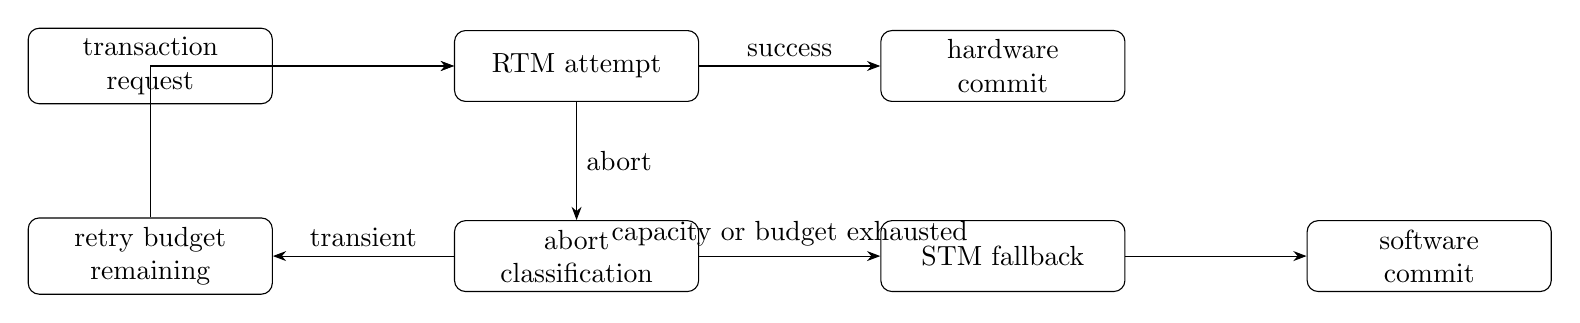
\begin{tikzpicture}[
    node distance=15mm and 23mm,
    >=Stealth,
    state/.style={draw, rounded corners, align=center, minimum width=31mm, minimum height=9mm}
]
\node[state] (start) {transaction\\request};
\node[state, right=of start] (rtm) {RTM attempt};
\node[state, right=of rtm] (hwcommit) {hardware\\commit};
\node[state, below=of rtm] (classify) {abort\\classification};
\node[state, left=of classify] (retry) {retry budget\\remaining};
\node[state, right=of classify] (stm) {STM fallback};
\node[state, right=of stm] (swcommit) {software\\commit};

\draw[->] (start) -- (rtm);
\draw[->] (rtm) -- node[above]{success} (hwcommit);
\draw[->] (rtm) -- node[right]{abort} (classify);
\draw[->] (classify) -- node[above]{transient} (retry);
\draw[->] (retry) |- (rtm);
\draw[->] (classify) -- node[above]{capacity or budget exhausted} (stm);
\draw[->] (stm) -- (swcommit);
\end{tikzpicture}
}%

\caption{A phased hybrid state machine. The research problem is not the branch itself, but the ownership contract between the RTM path and the STM fallback.}
\label{fig:phased-hybrid-state}
\end{figure}
\section{Summary}
\begin{itemize}
    \item TM is a rich research field with many unsolved problems.
    \item The student should leave with a critical understanding of where TM stands and where it might go.
    \item Directions worth watching divide into three families: hardware (hybrid HTM, GPU), systems (persistent, distributed), and methods (verification, education).
    \item Read this chapter as a \emph{synthesis organised around where the book's own codebase stops working}, not as a disconnected wish-list. The limits that surface in each family are the same limits the earlier parts hit: HTM's capacity aborts (Ch.~16), STM's validation and reclamation costs (Ch.~9, 13), the missing compiler/language contract (Ch.~11), and the absence of coherence on GPUs (Ch.~17). Each open direction in this chapter is one of those known limits restated as a research target.
\end{itemize}

\section{Exercises}
\begin{enumerate}
    \item Evaluate whether a hybrid TM that starts in hardware and falls back to software is inherently more susceptible to livelock than a pure-STM system.
    \item Propose a minimal extension to a persistent-memory TM that ensures durability of committed transactions across power failures.
    \item Argue for or against: “Transactional memory will eventually replace locks as the default concurrency primitive in systems programming.”
    \item \emph{[theory]} Classify the phased hybrid in Figure~\ref{fig:phased-hybrid-state} under obstruction freedom, starvation freedom, and lock freedom. State which assumptions about retry bounds, fallback admission, and conflict ownership are necessary for each classification.
\end{enumerate}

% -------------------------------------------------------------------
%  APPENDICES
% -------------------------------------------------------------------
\appendix

\chapter{Notation}

\begin{description}
    \item[$\lambda$] arrival rate of transactions (Little's Law, \S\ref{sec:math-example}).
    \item[$S$] average service time of one transaction attempt.
    \item[$L$] average number of in-flight transactions; $L = \lambda S$.
    \item[$p$ or $p_{abort}$] probability that an attempt aborts; expected
          attempts $= 1/(1-p)$ (geometric distribution).
    \item[$\mathit{rs}$, $\mathit{ws}$] read set, write set of a transaction.
    \item[$T_1, T_2, \ldots$] individual transactions in a history.
    \item[$\prec$] precedes, in a serial order of transactions.
    \item[$\mathrm{startTS}$] the GTS snapshot a GUST transaction takes at
          begin (\S\ref{sec:snapshot-example}).
    \item[\texttt{Active}, \texttt{Validating}, \texttt{Committed},
          \texttt{Aborted}] the four lifecycle states of \S\ref{sec:math-example}.
\end{description}

\chapter{Acronyms}

\begin{description}
    \item[CCT] Concurrently-Committing-Transaction (GUST).
    \item[CSMV] Client--Server Multi-Version \cite{nunes22csmv}.
    \item[DSE] Dead-Store Elimination.
    \item[GTS] Global Timestamp (GUST).
    \item[HTM] Hardware Transactional Memory.
    \item[JVSTM] Java Versioned Software Transactional Memory (multi-version) \cite{cachopo06}.
    \item[LICM] Loop-Invariant Code Motion.
    \item[MRV] Most-Recent-Version (GUST).
    \item[MVLog] Multi-Version Commit-Log STM (this book, Part~IV).
    \item[NOrec] NO Ownership RECords (value-based validation).
    \item[OCC] Optimistic Concurrency Control.
    \item[RTM] Restricted Transactional Memory (Intel).
    \item[SGL] Single Global Lock.
    \item[STM] Software Transactional Memory.
    \item[TLA+ / PlusCal] Temporal Logic of Actions; the PlusCal algorithmic notation compiled to TLA+.
    \item[TLC] The TLA+ model checker.
    \item[TL2] Transactional Locking II (global-clock OCC).
    \item[TM] Transactional Memory.
    \item[TSO] Total Store Order.
    \item[TSX] Transactional Synchronization Extensions (Intel).
    \item[VBox] Versioned Box.
\end{description}

% -------------------------------------------------------------------
\chapter{Glossary}
\label{chap:glossary}
Terms are defined in the chapter or section named in \emph{see}. Entries marked
[TSX] refer to Intel RTM; [GPU] to Part~VII.

\begin{description}
    \item[abort] \index{abort} The discard of a transaction's speculative
          writes and restart of its body. Opposed to \emph{commit}
          (\S\ref{sec:api-example}).
    \item[atomic block] \index{atomic block} A programming-language construct
          whose body is executed transactionally; see \S\ref{sec:atomics-example}.
    \item[ballot] \index{ballot} \texttt{\_\_ballot\_sync}, the GPU primitive
          that collects one predicate bit per lane into a mask
          (\S\ref{sec:ballot}).
    \item[commit] \index{commit} The point at which a transaction's writes
          become visible atomically (\S\ref{sec:tl2-example}).
    \item[commit log] \index{commit log} A bounded global record of in-flight
          transactions used by GPU designs such as GUST for CCT/MRV
          validation (\S\ref{sec:gust}).
    \item[CCT] \index{CCT} Concurrently-Committing-Transaction checking; GUST's
          validation of a commit against still-in-flight transactions
          (\S\ref{sec:gust}).
    \item[deadlock] \index{deadlock} A state in which every participant waits
          on another and no progress is possible (Part~I).
    \item[divergence] \index{divergence} In SIMT execution, lanes of a warp
          taking different control paths (\S\ref{sec:ballot}).
    \item[fallback] \index{fallback} The software path a best-effort HTM takes
          when hardware speculation aborts (\S\ref{sec:rtm-example}).
    \item[global clock] \index{global clock} A monotonically increasing
          version counter used by TL2 and NOrec to stamp commits
          (\S\ref{sec:norec-example}).
    \item[GTS] \index{GTS} Global Timestamp in GUST; counts finalized commit-log
          slots (\S\ref{sec:gust}).
    \item[intra-warp conflict] \index{intra-warp conflict} A conflict between
          lanes of the same warp, resolved by predicate voting
          (\S\ref{sec:ballot-example}).
    \item[linearizability / serializability] \index{serializability} The
          guarantee that a history is equivalent to some serial execution
          (\S\ref{sec:tso-example}).
    \item[liveness] \index{liveness} The guarantee that a good state is
          eventually reached; contrasted with \emph{safety}
          (\S\ref{sec:pluscal-example}).
    \item[MRV] \index{MRV} Most-Recent-Version checking; GUST's validation of
          finalised transactions via their latest VBox bodies
          (\S\ref{sec:gust}).
    \item[opacity] \index{opacity} Opacity ensures aborted transactions see a
          consistent state; a serializable-but-not-opaque history is dismantled
          in \S\ref{sec:tso-example}.
    \item[read set / write set] \index{read set} \index{write set} The
          addresses a transaction reads and writes; maintained by the runtime
          during the body (\S\ref{sec:norec-example}).
    \item[read-validate] \index{read-validate} The capture$\rightarrow$read
          $\rightarrow$recheck discipline that prevents partially-visible
          writes (\S\ref{sec:norec-example}).
    \item[retry loop] \index{retry loop} The \texttt{sigsetjmp}/
          \texttt{siglongjmp} machinery that restarts aborted transactions
          (\S\ref{sec:jmpbuf-example}).
    \item[safety] \index{safety} The guarantee that a bad state is never
          reached; contrasted with \emph{liveness} (\S\ref{sec:pluscal-example}).
    \item[simulation (CPU)] \index{simulation} Time-discrete execution of a
          trace or model to predict a design's behaviour (Parts~I, III, and VI).
    \item[store buffer] \index{store buffer} A per-core FIFO that delays store
          visibility, the source of TSO reordering (\S\ref{sec:tso-example}).
    \item[TSX] \index{TSX} Intel Transactional Synchronization Extensions; the
          RTM \texttt{xbegin}/\texttt{xend} instruction pair
          (\S\ref{sec:rtm-example}).
    \item[VBox] \index{VBox} Versioned box; per-address history of
          (version, value) bodies used by JVSTM, GUST, and other multi-version
          STMs (\S\ref{sec:gust}).
    \item[versioned box] \index{versioned box} \emph{See} VBox.
\end{description}

% -------------------------------------------------------------------
\chapter{PlusCal / TLA+ Quick Reference}
\begin{itemize}
    \item Key language constructs: variables, actions, labels, \texttt{either/or}, invariants, properties.
    \item Common TLC commands: \texttt{tlc -config model.cfg model.tla}, invariant checks, \texttt{-deadlock}.
    \item Writing a config file: constants, invariants, properties, \texttt{Init}/\texttt{Next}.
    \item Typical TM model skeleton: a thread (process), per-thread read/write set, global clock, and an opacity invariant.
    \item Pitfalls in practice: fingerprinting record-valued state, unbounded state spaces, and PlusCal `missing label' errors.
    \item How to read a counterexample trace: step-by-step from violation to root cause.
\end{itemize}

\chapter{TikZ Drawing Guide}
\begin{itemize}
    \item How to draw pipelines, caches, state machines, and Markov chains.
    \item Reusable templates.
    \item Common TM figures used in this book: transaction-lifecycle state machine, cache-coherence conflict diagram, clock/read-set validation timeline, abort/retry waveform.
    \item Timeline pattern showing which clock values reads observe during validation (used in the TL2 section of Part~IV).
    \item Warp-divergence and ballot diagrams for Part~VII.
    \item Style guide: reuse a small accent palette so figures stay visually consistent.
\end{itemize}

\chapter{Development Environment Setup}
\begin{itemize}
    \item Installing LLVM, GCC, TLA+ Toolbox, \texttt{rr}, gem5.
    \item Building the companion runtime with CMake, selecting a backend, and running the test targets.
    \item Running the STAMP benchmarks and reading their output (aborts, throughput, invariants).
    \item Model-checking workflow: translate PlusCal, run TLC, inspect a counterexample, fix the design.
    \item GPU toolchains (CUDA/ROCm, nvcc/hipcc) and where the GPU backends require dedicated hardware.
    \item Common failure modes and their fixes: DATA/TEXT symbol collisions, region-address conflicts, missing LLVM target flags.
\end{itemize}

\chapter{Answers and Hints for Selected Exercises}
\begin{itemize}
    \item Brief solutions or pointers to the main text where the concept is explained.
    \item One concise hint per exercise, referencing the section that resolves it.
    \item For model-checking exercises, hint at the invariant name and the bound that keeps TLC fast.
    \item For implementation exercises, point at the companion code location and the command that verifies the solution.
\end{itemize}

% -------------------------------------------------------------------
% ~~~~~~~~~~~~~~ Back matter ~~~~~~~~~~~~~~
\backmatter
\bibliographystyle{plain}
\bibliography{references}

\printindex

\end{document}